\documentclass[a4paper, 11pt, twoside=semi]{scrartcl}

\usepackage[utf8]{inputenc}
\usepackage[english]{babel}

\usepackage{enumerate}

% Deutsche Silbentrennung
%\usepackage[ngerman]{babel}

% Typische Mathesymbole etc, was man oft braucht
\usepackage{textcomp}
\usepackage{latexsym}
\usepackage{amssymb}
\usepackage{amsmath}
\usepackage{wasysym}
%\usepackage{txfonts}

% Teilfiguren in figure Umgebungen erlauben%
\usepackage{subfig}
\usepackage{float}
\restylefloat{figure}

% Schrift die mit Zeichencodierung klar kommt
%\usepackage{lmodern}




% Bilder einfügen
\usepackage{graphicx}
% Quelltext einfügen
\usepackage{verbatim}
%allows multiple rows and colums in a tabular environment
\usepackage{array}
%\usepackage{multirow}
\usepackage{multicol}


%fancy haedings
%\usepackage{fancyhdr}
%\pagestyle{fancy}

% Definitionen von Farben
\usepackage{xcolor}
\definecolor{LinkColor}{rgb}{0,0,0.5}
\definecolor{blue}{rgb}{0,0,1}
% \definecolor{dkgreen}{rgb}{0,0.6,0}
% \definecolor{gray}{rgb}{0.5,0.5,0.5}
% \definecolor{mauve}{rgb}{0.58,0,0.82}

% Einf\"ugen von Tikz grafiken
\usepackage{booktabs}
\usepackage{pgf}
\usepackage{tikz}
\usetikzlibrary{shapes,backgrounds,mindmap,trees,calc}

\usepackage{pgfplots}
%\usepackage{pgfplotstable}
%\usepgfplotslibrary{colormaps}
%\usepgfplotslibrary{colorbrewer}
\usetikzlibrary{pgfplots.colorbrewer}
\pgfplotsset{compat=1.15} %
\pgfplotsset{cycle list/PiYG}
\pgfplotsset{cycle list/Spectral}
\pgfplotsset{cycle list/Greys}

%\usepackage{filecontents}

\newcounter{piea}
\newcounter{pieb}
\newcounter{piec}
\newcounter{pied}
\newcounter{piee}
\newcounter{pief}
\newcounter{pieg}
\newcounter{pieh}



% Definitionen f\"ur Spiderweb chart
\newcommand{\D}{5} % number of dimensions (config option)
\newcommand{\U}{100} % number of scale units (config option)
\newcommand{\US}{5}   % number of scale units shown (config option)
\newdimen\R % maximal diagram radius (config option)
\R=2cm 
\newdimen\L % radius to put dimension labels (config option)
\L=3cm
\newcommand{\A}{360/\D} % calculated angle between dimension axes  
\newcommand{\SU}{\U/\US} % calculated distance between shown axes  
\newcommand{\createradar}{
  \path (0:0cm) coordinate (O); % define coordinate for origin
  % draw the spiderweb
  \foreach \X in {1,...,\D}{ \draw [opacity=.5] (\X*\A+90:0) -- (\X*\A+90:\R); }%
  \foreach \Y in {0,...,\U}{ \foreach \X in {1,...,\D}{ \path (\X*\A+90:\Y*\R/\U) coordinate (D\X-\Y); } } %
  \foreach \Y in {0,...,\US}{ \foreach \X in {1,...,\D}{ \path (\X*\A+90:\Y*\SU*\R/\U) coordinate (A\X-\Y); \fill [opacity=0.5] (A\X-\Y) circle (1pt); }%
                              \draw [opacity=0.5] (0+90:\Y*\SU*\R/\U) \foreach \X in {1,...,\D}{ -- (\X*\A+90:\Y*\SU*\R/\U)  } -- cycle; }%  
  %create correct width
  \draw [color=white] (-5,2) -- (5,2);%
  % define labels for each dimension axis (names config option)
  \path (1*\A+90:\L) node (L1) {\small Heterogenit\"at};%
  \path (2*\A+90:.85\L) node (L2) {\small Verteilung};%
  \path (3*\A+90:.87\L) node (L3) {\small Zeitabh\"angigkeit};%
  \path (4*\A+90:\L) node (L4) {\small Dynamik};%
  \path (5*\A+90:.8\L) node (L5) {\small Komplexit\"at};%  
}

% Definition for Pie-Chart
\newcommand{\slice}[5]{%
  \pgfmathparse{0.5*#1+0.5*#2}%
  \let\midangle\pgfmathresult%
  % slice
  \draw[thin,fill=#5,draw=white] (0,0) -- (#1:1) arc (#1:#2:1) -- cycle;%
  % outer label
  \node[label=\midangle:#4] at (\midangle:1) {};%
  % inner label
  \pgfmathparse{min((#2-#1-10)/110*(-0.3),0)}%
  \let\temp\pgfmathresult%
  \pgfmathparse{max(\temp,-0.5) + 0.8}%
  \let\innerpos\pgfmathresult%
  \node at (\midangle:\innerpos) {#3};%
}

%Definition of Box-Plots
\newcommand{\boxplot}[6]{%
	%#1: center, #2: median, #3: 1/4 quartile, #4: 3/4 quartile, #5: min, #6: max
	\filldraw[fill=blue!30,draw=blue,line width=.2mm] let \n{boxxl}={#1-0.3}, \n{boxxr}={#1+0.3} in (axis cs:\n{boxxl},#3) rectangle (axis cs:\n{boxxr},#4);   % draw the box
	\draw[line width=1mm, color=blue] let \n{boxxl}={#1-0.3}, \n{boxxr}={#1+0.3} in (axis cs:\n{boxxl},#2) -- (axis cs:\n{boxxr},#2);             % median
	\draw[line width=.2mm] (axis cs:#1,#4) -- (axis cs:#1,#6);                                                                           % bar up
	\draw[line width=.2mm] let \n{whiskerl}={#1-0.15}, \n{whiskerr}={#1+0.15} in (axis cs:\n{whiskerl},#6) -- (axis cs:\n{whiskerr},#6);        % upper quartile
	\draw[line width=.2mm] (axis cs:#1,#3) -- (axis cs:#1,#5);                                                                           % bar down
	\draw[line width=.2mm] let \n{whiskerl}={#1-0.15}, \n{whiskerr}={#1+0.15} in (axis cs:\n{whiskerl},#5) -- (axis cs:\n{whiskerr},#5);        % lower quartile
}


% Definition der Befehle todo und todoln fuer Hinweistexte
%\newcommand\todo[1]{\fbox{\scriptsize\textbf{#1}}}
%\newcommand\todoln[1]{\fbox{\parbox{.9\linewidth}{\scriptsize\textbf{#1}}}}


\author{Thomas Kühn}
\title{Evaluation @ ECSA\&ICSA}


\begin{document}

\section{Paper Class}

%\subsection{Histogramm f\"ur Paper class (199)}
%\begin{figure}
\begin{center}
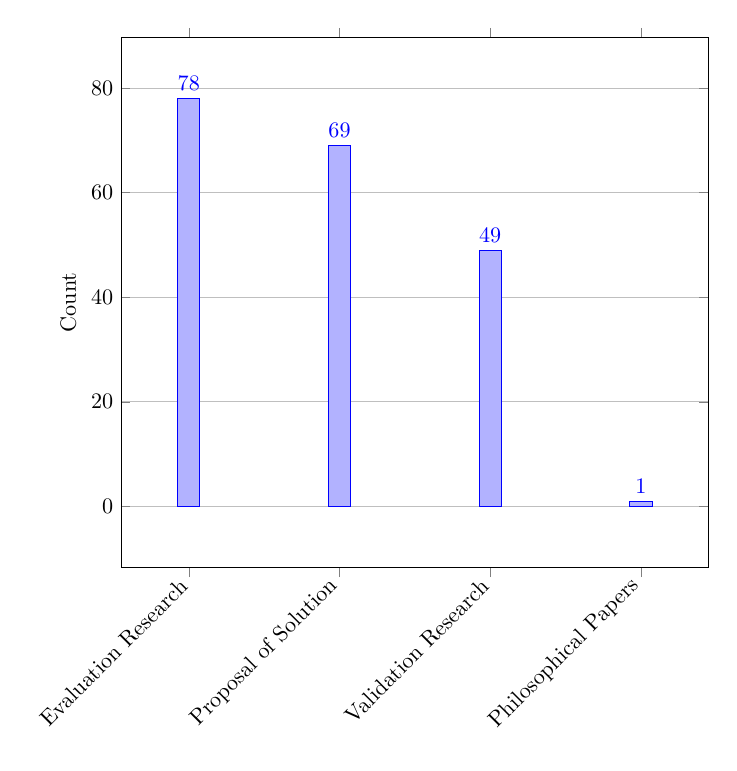
\begin{tikzpicture}[scale=.8]
\begin{axis}[ ybar, ymajorgrids, enlargelimits=0.15, legend style={at={(0.5,-0.15)}, anchor=north,legend columns=-1},
    width=.90\linewidth,height=10cm,
    nodes near coords, %nodes near coords align=below,
    ylabel={Count}, ymin=0,
    x tick label style={rotate=45,anchor=east},
    xtick={1,2,3,4},
    xticklabels={Evaluation Research,Proposal of Solution,Validation Research,Philosophical Papers
}
    %xlabel={Paper class}    
    ]
  \addplot coordinates { (1,78)  (2,69)  (3,49)  (4,1)   };
\end{axis}
\end{tikzpicture}
\end{center}
%\caption{Histogramm f\"ur Paper class (199)}
%\label{fig:histo_paperclass}
%\end{figure}



%\subsection{Pie chart for Paper class (197)}
%\begin{figure}
\begin{center}
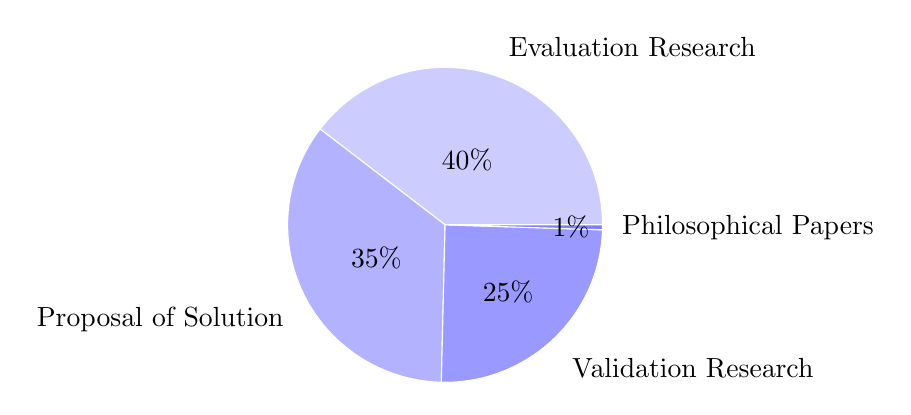
\begin{tikzpicture}[scale=2]
\pgfmathsetcounter{pieb}{0}
\foreach \p/\q/\t/\c in {40/78/Evaluation Research/blue!20, 35/69/Proposal of Solution/blue!30, 25/49/Validation Research/blue!40, 1/1/Philosophical Papers/blue!50}
  {
    \setcounter{piea}{\value{pieb}}
    \addtocounter{pieb}{\q}
    \slice{\thepiea/197*360}
          {\thepieb/197*360}
          {\p\%}{\t}{\c}
  }
\end{tikzpicture}
\textbf{Pie chart for Paper class (197)}
\end{center}
%\caption{Pie chart for Paper class (197)}
%\label{fig:pie_paperclass}
%\end{figure}


%\subsection{Histogram von Year je Paper class}
%\begin{figure}
\begin{center}
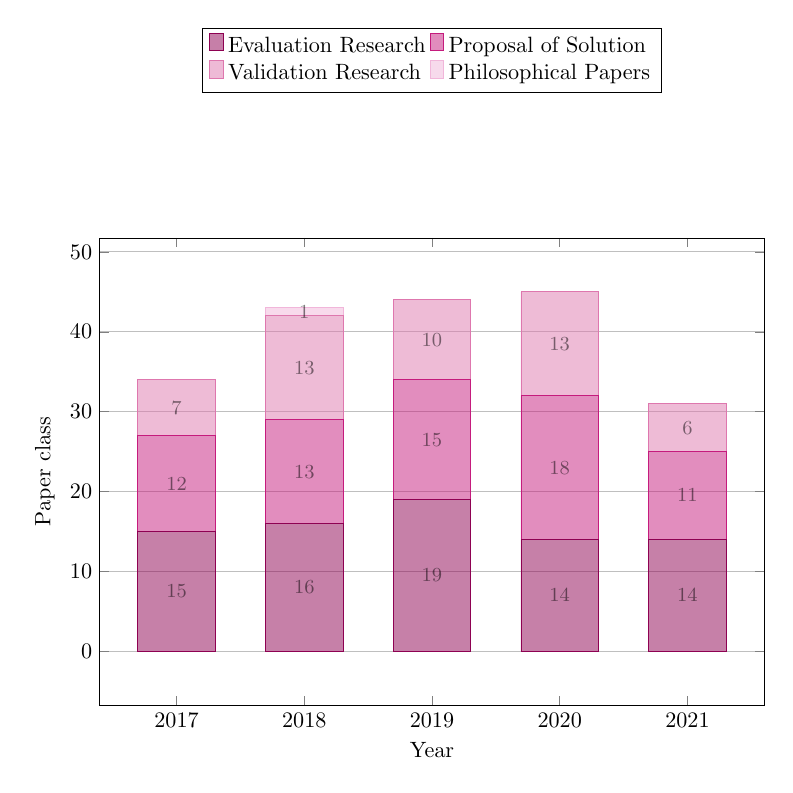
\begin{tikzpicture}[scale=0.8]
\
\begin{axis}[ width=\linewidth, height=9cm, ybar stacked,
    cycle list name=PiYG,
    every axis plot/.append style={draw,fill,fill opacity=0.5},
    nodes near coords, %nodes near coords align=below,
    nodes near coords style={color=black,font=\small},
    enlargelimits=0.15, 
    bar width=3.5em,
    legend style={at={(0.5,1.45)}, anchor=north,legend columns=2},
    legend cell align={left},
    ylabel={Paper class},ymajorgrids,ymin=0,
    %x tick label style={rotate=45,anchor=east},
    xtick={1,2,3,4,5}, xticklabels={2017,2018,2019,2020,2021},
    xlabel={Year}    
   ]
\addplot coordinates { (1,15)  (2,16)  (3,19)  (4,14)  (5,14)  };
\addplot coordinates { (1,12)  (2,13)  (3,15)  (4,18)  (5,11)  };
\addplot coordinates { (1,7)  (2,13)  (3,10)  (4,13)  (5,6)  };
\addplot coordinates { (1,0)  (2,1)  (3,0)  (4,0)  (5,0)  };

\legend{Evaluation Research,Proposal of Solution,Validation Research,Philosophical Papers}
\end{axis}
\end{tikzpicture}
\end{center}
%\caption{Histogram von Year je Paper class}
%\label{fig:chisto_year_paperclass}
%\end{figure}


%\subsection{Portfolio f\"ur Year und Paper class (Gr\"o\ss{}e entspricht der Anzahl)}
%\begin{figure}
\begin{center}
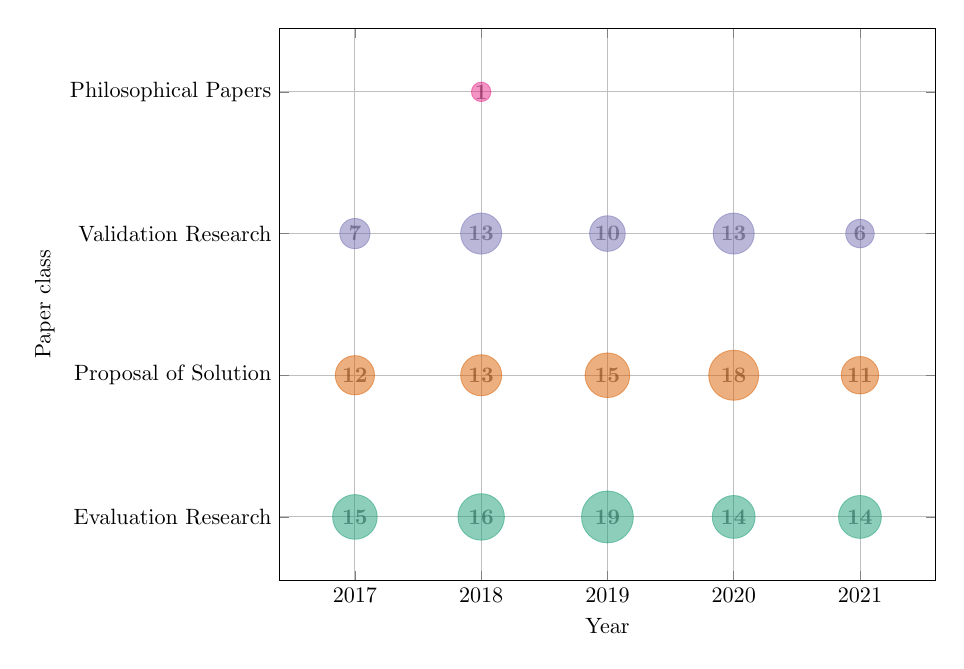
\begin{tikzpicture}[scale=.8]
\pgfplotsset{cycle list/Dark2}
\begin{axis}[width=.99\linewidth,
    enlargelimits=0.15,
    %x tick label style={rotate=45,anchor=east},
    xtick={0,1,2,3,4}, xticklabels={2017,2018,2019,2020,2021},
    xlabel={Year},
    ytick={0,1,2,3}, yticklabels={Evaluation Research,Proposal of Solution,Validation Research,Philosophical Papers},
    ylabel={Paper class},
    grid=both,
    scatter,scatter src=y,
    scatter/classes={0={draw=Dark2-A,fill=Dark2-A}, 1={draw=Dark2-B,fill=Dark2-B}, 2={draw=Dark2-C,fill=Dark2-C}, 3={draw=Dark2-D,fill=Dark2-D}}
]

\addplot+[mark=*,mark size=10.091,opacity=0.5,text=black] coordinates { (0,0) } node[text=black,font=\bfseries] {15};
\addplot+[mark=*,mark size=8.873,opacity=0.5,text=black] coordinates { (0,1) } node[text=black,font=\bfseries] {12};
\addplot+[mark=*,mark size=6.843,opacity=0.5,text=black] coordinates { (0,2) } node[text=black,font=\bfseries] {7};
\addplot+[mark=*,mark size=10.497,opacity=0.5,text=black] coordinates { (1,0) } node[text=black,font=\bfseries] {16};
\addplot+[mark=*,mark size=9.279,opacity=0.5,text=black] coordinates { (1,1) } node[text=black,font=\bfseries] {13};
\addplot+[mark=*,mark size=9.279,opacity=0.5,text=black] coordinates { (1,2) } node[text=black,font=\bfseries] {13};
\addplot+[mark=*,mark size=4.406,opacity=0.5,text=black] coordinates { (1,3) } node[text=black,font=\bfseries] {1};
\addplot+[mark=*,mark size=11.716,opacity=0.5,text=black] coordinates { (2,0) } node[text=black,font=\bfseries] {19};
\addplot+[mark=*,mark size=10.091,opacity=0.5,text=black] coordinates { (2,1) } node[text=black,font=\bfseries] {15};
\addplot+[mark=*,mark size=8.061,opacity=0.5,text=black] coordinates { (2,2) } node[text=black,font=\bfseries] {10};
\addplot+[mark=*,mark size=9.685,opacity=0.5,text=black] coordinates { (3,0) } node[text=black,font=\bfseries] {14};
\addplot+[mark=*,mark size=11.310,opacity=0.5,text=black] coordinates { (3,1) } node[text=black,font=\bfseries] {18};
\addplot+[mark=*,mark size=9.279,opacity=0.5,text=black] coordinates { (3,2) } node[text=black,font=\bfseries] {13};
\addplot+[mark=*,mark size=9.685,opacity=0.5,text=black] coordinates { (4,0) } node[text=black,font=\bfseries] {14};
\addplot+[mark=*,mark size=8.467,opacity=0.5,text=black] coordinates { (4,1) } node[text=black,font=\bfseries] {11};
\addplot+[mark=*,mark size=6.437,opacity=0.5,text=black] coordinates { (4,2) } node[text=black,font=\bfseries] {6};


\end{axis}
\end{tikzpicture}
\end{center}
%\caption{Portfolio f\"ur Year und Paper class (Gr\"o\ss{}e entspricht der Anzahl)}\label{fig:port_year_paperclass}
%\end{figure}



\section{Research Objects}

%\subsection{Histogramm f\"ur Research Object (171)}
%\begin{figure}
\begin{center}
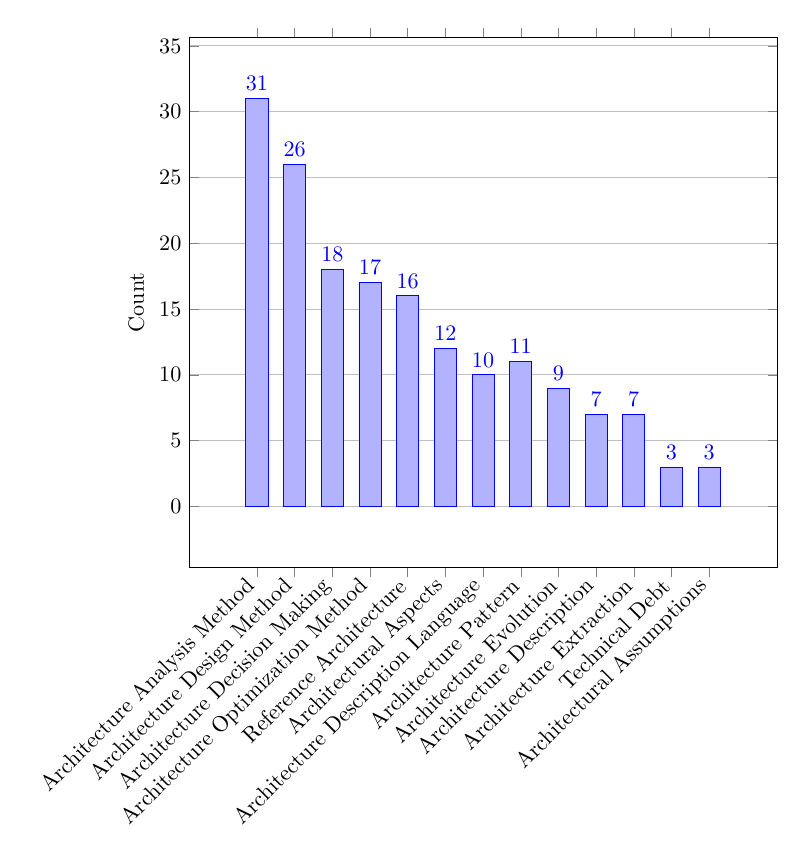
\begin{tikzpicture}[scale=.8]
\begin{axis}[ ybar, ymajorgrids, enlargelimits=0.15, legend style={at={(0.5,-0.15)}, anchor=north,legend columns=-1},
    width=.90\linewidth,height=10cm,
    nodes near coords, %nodes near coords align=below,
    ylabel={Count}, ymin=0,
    x tick label style={rotate=45,anchor=east},
    xtick={1,2,3,4,5,6,7,8,9,10,11,12,13},
    xticklabels={Architecture Analysis Method,Architecture Design Method,Architecture Decision Making,Architecture Optimization Method,Reference Architecture,Architectural Aspects,Architecture Description Language,Architecture Pattern,Architecture Evolution,Architecture Description,Architecture Extraction,Technical Debt,Architectural Assumptions
}
    %xlabel={Research Object}    
    ]
  \addplot coordinates { (1,31)  (2,26)  (3,18)  (4,17)  (5,16)  (6,12)  (7,10)  (8,11)  (9,9)  (10,7)  (11,7)  (12,3)  (13,3)   };
\end{axis}
\end{tikzpicture}
\end{center}
%\caption{Histogramm f\"ur Research Object (171)}
%\label{fig:histo_researchobject}
%\end{figure}



%\subsection{Pie chart for Research Object (170)}
%\begin{figure}
\begin{center}
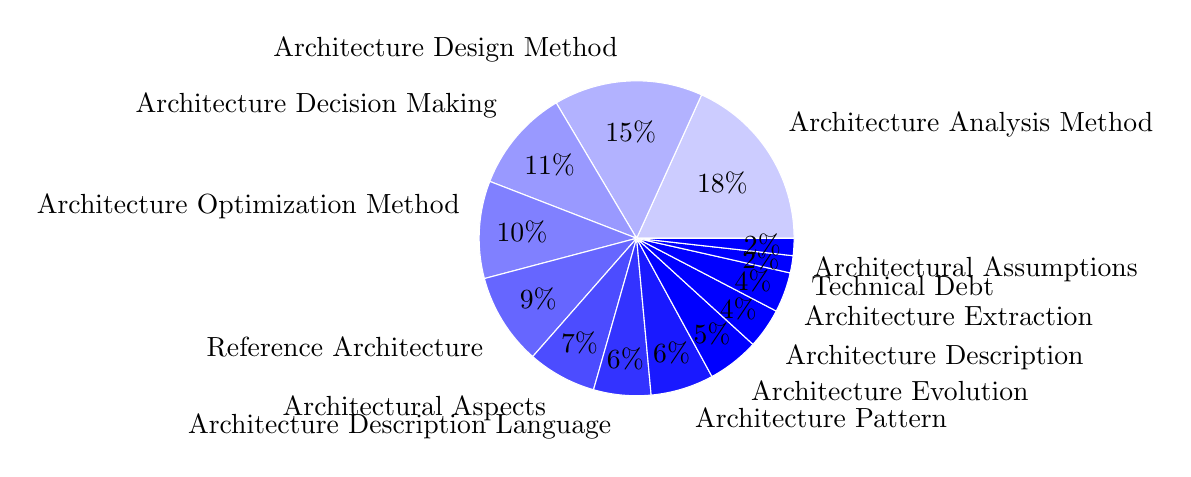
\begin{tikzpicture}[scale=2]
\pgfmathsetcounter{pieb}{0}
\foreach \p/\q/\t/\c in {18/31/Architecture Analysis Method/blue!20, 15/26/Architecture Design Method/blue!30, 11/18/Architecture Decision Making/blue!40, 10/17/Architecture Optimization Method/blue!50, 9/16/Reference Architecture/blue!60, 7/12/Architectural Aspects/blue!70, 6/10/Architecture Description Language/blue!80, 6/11/Architecture Pattern/blue!90, 5/9/Architecture Evolution/blue!100, 4/7/Architecture Description/blue!110, 4/7/Architecture Extraction/blue!120, 2/3/Technical Debt/blue!130, 2/3/Architectural Assumptions/blue!140}
  {
    \setcounter{piea}{\value{pieb}}
    \addtocounter{pieb}{\q}
    \slice{\thepiea/170*360}
          {\thepieb/170*360}
          {\p\%}{\t}{\c}
  }
\end{tikzpicture}
\textbf{Pie chart for Research Object (170)}
\end{center}
%\caption{Pie chart for Research Object (170)}
%\label{fig:pie_researchobject}
%\end{figure}


%\subsection{Histogram von Year je Research Object}
%\begin{figure}
\begin{center}
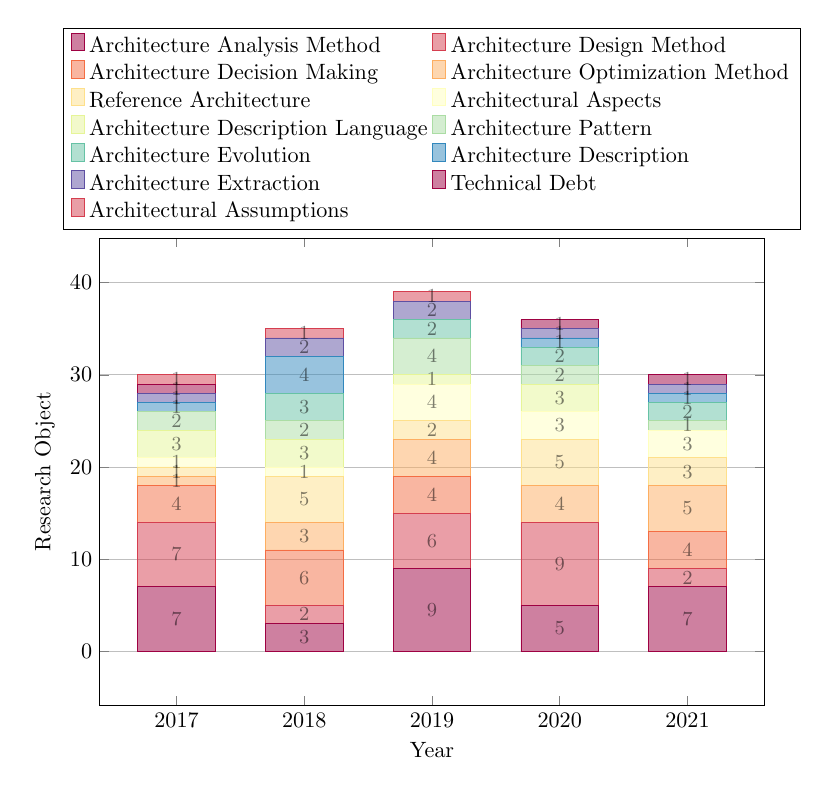
\begin{tikzpicture}[scale=0.8]
\
\begin{axis}[ width=\linewidth, height=9cm, ybar stacked,
    cycle multi list=Spectral,
    every axis plot/.append style={draw,fill,fill opacity=0.5},
    nodes near coords, %nodes near coords align=below,
    nodes near coords style={color=black,font=\small},
    enlargelimits=0.15, 
    bar width=3.5em,
    legend style={at={(0.5,1.45)}, anchor=north,legend columns=2},
    legend cell align={left},
    ylabel={Research Object},ymajorgrids,ymin=0,
    %x tick label style={rotate=45,anchor=east},
    xtick={1,2,3,4,5}, xticklabels={2017,2018,2019,2020,2021},
    xlabel={Year}    
   ]
\addplot coordinates { (1,7)  (2,3)  (3,9)  (4,5)  (5,7)  };
\addplot coordinates { (1,7)  (2,2)  (3,6)  (4,9)  (5,2)  };
\addplot coordinates { (1,4)  (2,6)  (3,4)  (4,0)  (5,4)  };
\addplot coordinates { (1,1)  (2,3)  (3,4)  (4,4)  (5,5)  };
\addplot coordinates { (1,1)  (2,5)  (3,2)  (4,5)  (5,3)  };
\addplot coordinates { (1,1)  (2,1)  (3,4)  (4,3)  (5,3)  };
\addplot coordinates { (1,3)  (2,3)  (3,1)  (4,3)  (5,0)  };
\addplot coordinates { (1,2)  (2,2)  (3,4)  (4,2)  (5,1)  };
\addplot coordinates { (1,0)  (2,3)  (3,2)  (4,2)  (5,2)  };
\addplot coordinates { (1,1)  (2,4)  (3,0)  (4,1)  (5,1)  };
\addplot coordinates { (1,1)  (2,2)  (3,2)  (4,1)  (5,1)  };
\addplot coordinates { (1,1)  (2,0)  (3,0)  (4,1)  (5,1)  };
\addplot coordinates { (1,1)  (2,1)  (3,1)  (4,0)  (5,0)  };

\legend{Architecture Analysis Method,Architecture Design Method,Architecture Decision Making,Architecture Optimization Method,Reference Architecture,Architectural Aspects,Architecture Description Language,Architecture Pattern,Architecture Evolution,Architecture Description,Architecture Extraction,Technical Debt,Architectural Assumptions}
\end{axis}
\end{tikzpicture}
\end{center}
%\caption{Histogram von Year je Research Object}
%\label{fig:chisto_year_researchobject}
%\end{figure}


%\subsection{Portfolio f\"ur Year und Research Object (Gr\"o\ss{}e entspricht der Anzahl)}
%\begin{figure}
\begin{center}
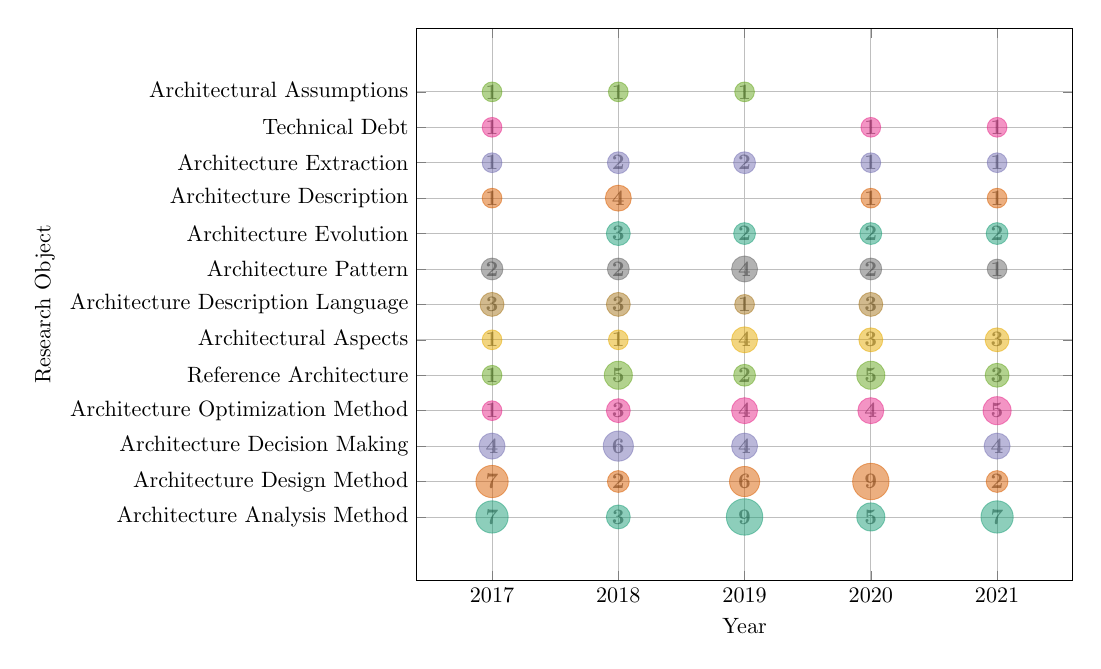
\begin{tikzpicture}[scale=.8]
\pgfplotsset{cycle list/Dark2}
\begin{axis}[width=.99\linewidth,
    enlargelimits=0.15,
    %x tick label style={rotate=45,anchor=east},
    xtick={0,1,2,3,4}, xticklabels={2017,2018,2019,2020,2021},
    xlabel={Year},
    ytick={0,1,2,3,4,5,6,7,8,9,10,11,12}, yticklabels={Architecture Analysis Method,Architecture Design Method,Architecture Decision Making,Architecture Optimization Method,Reference Architecture,Architectural Aspects,Architecture Description Language,Architecture Pattern,Architecture Evolution,Architecture Description,Architecture Extraction,Technical Debt,Architectural Assumptions},
    ylabel={Research Object},
    grid=both,
    scatter,scatter src=y,
    scatter/classes={0={draw=Dark2-A,fill=Dark2-A}, 1={draw=Dark2-B,fill=Dark2-B}, 2={draw=Dark2-C,fill=Dark2-C}, 3={draw=Dark2-D,fill=Dark2-D}, 4={draw=Dark2-E,fill=Dark2-E}, 5={draw=Dark2-F,fill=Dark2-F}, 6={draw=Dark2-G,fill=Dark2-G}, 7={draw=Dark2-H,fill=Dark2-H}, 8={draw=Dark2-A,fill=Dark2-A}, 9={draw=Dark2-B,fill=Dark2-B}, 10={draw=Dark2-C,fill=Dark2-C}, 11={draw=Dark2-D,fill=Dark2-D}, 12={draw=Dark2-E,fill=Dark2-E}}
]

\addplot+[mark=*,mark size=7.294,opacity=0.5,text=black] coordinates { (0,0) } node[text=black,font=\bfseries] {7};
\addplot+[mark=*,mark size=7.294,opacity=0.5,text=black] coordinates { (0,1) } node[text=black,font=\bfseries] {7};
\addplot+[mark=*,mark size=5.882,opacity=0.5,text=black] coordinates { (0,2) } node[text=black,font=\bfseries] {4};
\addplot+[mark=*,mark size=4.471,opacity=0.5,text=black] coordinates { (0,3) } node[text=black,font=\bfseries] {1};
\addplot+[mark=*,mark size=4.471,opacity=0.5,text=black] coordinates { (0,4) } node[text=black,font=\bfseries] {1};
\addplot+[mark=*,mark size=4.471,opacity=0.5,text=black] coordinates { (0,5) } node[text=black,font=\bfseries] {1};
\addplot+[mark=*,mark size=5.412,opacity=0.5,text=black] coordinates { (0,6) } node[text=black,font=\bfseries] {3};
\addplot+[mark=*,mark size=4.941,opacity=0.5,text=black] coordinates { (0,7) } node[text=black,font=\bfseries] {2};
\addplot+[mark=*,mark size=4.471,opacity=0.5,text=black] coordinates { (0,9) } node[text=black,font=\bfseries] {1};
\addplot+[mark=*,mark size=4.471,opacity=0.5,text=black] coordinates { (0,10) } node[text=black,font=\bfseries] {1};
\addplot+[mark=*,mark size=4.471,opacity=0.5,text=black] coordinates { (0,11) } node[text=black,font=\bfseries] {1};
\addplot+[mark=*,mark size=4.471,opacity=0.5,text=black] coordinates { (0,12) } node[text=black,font=\bfseries] {1};
\addplot+[mark=*,mark size=5.412,opacity=0.5,text=black] coordinates { (1,0) } node[text=black,font=\bfseries] {3};
\addplot+[mark=*,mark size=4.941,opacity=0.5,text=black] coordinates { (1,1) } node[text=black,font=\bfseries] {2};
\addplot+[mark=*,mark size=6.824,opacity=0.5,text=black] coordinates { (1,2) } node[text=black,font=\bfseries] {6};
\addplot+[mark=*,mark size=5.412,opacity=0.5,text=black] coordinates { (1,3) } node[text=black,font=\bfseries] {3};
\addplot+[mark=*,mark size=6.353,opacity=0.5,text=black] coordinates { (1,4) } node[text=black,font=\bfseries] {5};
\addplot+[mark=*,mark size=4.471,opacity=0.5,text=black] coordinates { (1,5) } node[text=black,font=\bfseries] {1};
\addplot+[mark=*,mark size=5.412,opacity=0.5,text=black] coordinates { (1,6) } node[text=black,font=\bfseries] {3};
\addplot+[mark=*,mark size=4.941,opacity=0.5,text=black] coordinates { (1,7) } node[text=black,font=\bfseries] {2};
\addplot+[mark=*,mark size=5.412,opacity=0.5,text=black] coordinates { (1,8) } node[text=black,font=\bfseries] {3};
\addplot+[mark=*,mark size=5.882,opacity=0.5,text=black] coordinates { (1,9) } node[text=black,font=\bfseries] {4};
\addplot+[mark=*,mark size=4.941,opacity=0.5,text=black] coordinates { (1,10) } node[text=black,font=\bfseries] {2};
\addplot+[mark=*,mark size=4.471,opacity=0.5,text=black] coordinates { (1,12) } node[text=black,font=\bfseries] {1};
\addplot+[mark=*,mark size=8.235,opacity=0.5,text=black] coordinates { (2,0) } node[text=black,font=\bfseries] {9};
\addplot+[mark=*,mark size=6.824,opacity=0.5,text=black] coordinates { (2,1) } node[text=black,font=\bfseries] {6};
\addplot+[mark=*,mark size=5.882,opacity=0.5,text=black] coordinates { (2,2) } node[text=black,font=\bfseries] {4};
\addplot+[mark=*,mark size=5.882,opacity=0.5,text=black] coordinates { (2,3) } node[text=black,font=\bfseries] {4};
\addplot+[mark=*,mark size=4.941,opacity=0.5,text=black] coordinates { (2,4) } node[text=black,font=\bfseries] {2};
\addplot+[mark=*,mark size=5.882,opacity=0.5,text=black] coordinates { (2,5) } node[text=black,font=\bfseries] {4};
\addplot+[mark=*,mark size=4.471,opacity=0.5,text=black] coordinates { (2,6) } node[text=black,font=\bfseries] {1};
\addplot+[mark=*,mark size=5.882,opacity=0.5,text=black] coordinates { (2,7) } node[text=black,font=\bfseries] {4};
\addplot+[mark=*,mark size=4.941,opacity=0.5,text=black] coordinates { (2,8) } node[text=black,font=\bfseries] {2};
\addplot+[mark=*,mark size=4.941,opacity=0.5,text=black] coordinates { (2,10) } node[text=black,font=\bfseries] {2};
\addplot+[mark=*,mark size=4.471,opacity=0.5,text=black] coordinates { (2,12) } node[text=black,font=\bfseries] {1};
\addplot+[mark=*,mark size=6.353,opacity=0.5,text=black] coordinates { (3,0) } node[text=black,font=\bfseries] {5};
\addplot+[mark=*,mark size=8.235,opacity=0.5,text=black] coordinates { (3,1) } node[text=black,font=\bfseries] {9};
\addplot+[mark=*,mark size=5.882,opacity=0.5,text=black] coordinates { (3,3) } node[text=black,font=\bfseries] {4};
\addplot+[mark=*,mark size=6.353,opacity=0.5,text=black] coordinates { (3,4) } node[text=black,font=\bfseries] {5};
\addplot+[mark=*,mark size=5.412,opacity=0.5,text=black] coordinates { (3,5) } node[text=black,font=\bfseries] {3};
\addplot+[mark=*,mark size=5.412,opacity=0.5,text=black] coordinates { (3,6) } node[text=black,font=\bfseries] {3};
\addplot+[mark=*,mark size=4.941,opacity=0.5,text=black] coordinates { (3,7) } node[text=black,font=\bfseries] {2};
\addplot+[mark=*,mark size=4.941,opacity=0.5,text=black] coordinates { (3,8) } node[text=black,font=\bfseries] {2};
\addplot+[mark=*,mark size=4.471,opacity=0.5,text=black] coordinates { (3,9) } node[text=black,font=\bfseries] {1};
\addplot+[mark=*,mark size=4.471,opacity=0.5,text=black] coordinates { (3,10) } node[text=black,font=\bfseries] {1};
\addplot+[mark=*,mark size=4.471,opacity=0.5,text=black] coordinates { (3,11) } node[text=black,font=\bfseries] {1};
\addplot+[mark=*,mark size=7.294,opacity=0.5,text=black] coordinates { (4,0) } node[text=black,font=\bfseries] {7};
\addplot+[mark=*,mark size=4.941,opacity=0.5,text=black] coordinates { (4,1) } node[text=black,font=\bfseries] {2};
\addplot+[mark=*,mark size=5.882,opacity=0.5,text=black] coordinates { (4,2) } node[text=black,font=\bfseries] {4};
\addplot+[mark=*,mark size=6.353,opacity=0.5,text=black] coordinates { (4,3) } node[text=black,font=\bfseries] {5};
\addplot+[mark=*,mark size=5.412,opacity=0.5,text=black] coordinates { (4,4) } node[text=black,font=\bfseries] {3};
\addplot+[mark=*,mark size=5.412,opacity=0.5,text=black] coordinates { (4,5) } node[text=black,font=\bfseries] {3};
\addplot+[mark=*,mark size=4.471,opacity=0.5,text=black] coordinates { (4,7) } node[text=black,font=\bfseries] {1};
\addplot+[mark=*,mark size=4.941,opacity=0.5,text=black] coordinates { (4,8) } node[text=black,font=\bfseries] {2};
\addplot+[mark=*,mark size=4.471,opacity=0.5,text=black] coordinates { (4,9) } node[text=black,font=\bfseries] {1};
\addplot+[mark=*,mark size=4.471,opacity=0.5,text=black] coordinates { (4,10) } node[text=black,font=\bfseries] {1};
\addplot+[mark=*,mark size=4.471,opacity=0.5,text=black] coordinates { (4,11) } node[text=black,font=\bfseries] {1};


\end{axis}
\end{tikzpicture}
\end{center}
%\caption{Portfolio f\"ur Year und Research Object (Gr\"o\ss{}e entspricht der Anzahl)}\label{fig:port_year_researchobject}
%\end{figure}


%%\subsection{Portfolio f\"ur Research Object und Year (Gr\"o\ss{}e entspricht der Anzahl)}
%\begin{figure}
\begin{center}
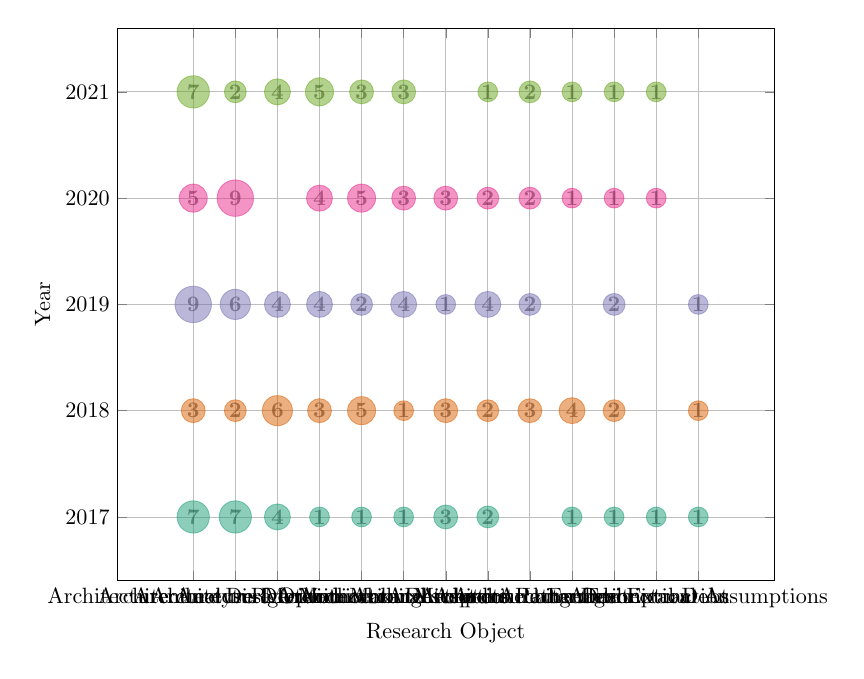
\begin{tikzpicture}[scale=.8]
\pgfplotsset{cycle list/Dark2}
\begin{axis}[width=.99\linewidth,
    enlargelimits=0.15,
    %x tick label style={rotate=45,anchor=east},
    xtick={0,1,2,3,4,5,6,7,8,9,10,11,12}, xticklabels={Architecture Analysis Method,Architecture Design Method,Architecture Decision Making,Architecture Optimization Method,Reference Architecture,Architectural Aspects,Architecture Description Language,Architecture Pattern,Architecture Evolution,Architecture Description,Architecture Extraction,Technical Debt,Architectural Assumptions},
    xlabel={Research Object},
    ytick={0,1,2,3,4}, yticklabels={2017,2018,2019,2020,2021},
    ylabel={Year},
    grid=both,
    scatter,scatter src=y,
    scatter/classes={0={draw=Dark2-A,fill=Dark2-A}, 1={draw=Dark2-B,fill=Dark2-B}, 2={draw=Dark2-C,fill=Dark2-C}, 3={draw=Dark2-D,fill=Dark2-D}, 4={draw=Dark2-E,fill=Dark2-E}}
]

\addplot+[mark=*,mark size=7.294,opacity=0.5,text=black] coordinates { (0,0) } node[text=black,font=\bfseries] {7};
\addplot+[mark=*,mark size=5.412,opacity=0.5,text=black] coordinates { (0,1) } node[text=black,font=\bfseries] {3};
\addplot+[mark=*,mark size=8.235,opacity=0.5,text=black] coordinates { (0,2) } node[text=black,font=\bfseries] {9};
\addplot+[mark=*,mark size=6.353,opacity=0.5,text=black] coordinates { (0,3) } node[text=black,font=\bfseries] {5};
\addplot+[mark=*,mark size=7.294,opacity=0.5,text=black] coordinates { (0,4) } node[text=black,font=\bfseries] {7};
\addplot+[mark=*,mark size=7.294,opacity=0.5,text=black] coordinates { (1,0) } node[text=black,font=\bfseries] {7};
\addplot+[mark=*,mark size=4.941,opacity=0.5,text=black] coordinates { (1,1) } node[text=black,font=\bfseries] {2};
\addplot+[mark=*,mark size=6.824,opacity=0.5,text=black] coordinates { (1,2) } node[text=black,font=\bfseries] {6};
\addplot+[mark=*,mark size=8.235,opacity=0.5,text=black] coordinates { (1,3) } node[text=black,font=\bfseries] {9};
\addplot+[mark=*,mark size=4.941,opacity=0.5,text=black] coordinates { (1,4) } node[text=black,font=\bfseries] {2};
\addplot+[mark=*,mark size=5.882,opacity=0.5,text=black] coordinates { (2,0) } node[text=black,font=\bfseries] {4};
\addplot+[mark=*,mark size=6.824,opacity=0.5,text=black] coordinates { (2,1) } node[text=black,font=\bfseries] {6};
\addplot+[mark=*,mark size=5.882,opacity=0.5,text=black] coordinates { (2,2) } node[text=black,font=\bfseries] {4};
\addplot+[mark=*,mark size=5.882,opacity=0.5,text=black] coordinates { (2,4) } node[text=black,font=\bfseries] {4};
\addplot+[mark=*,mark size=4.471,opacity=0.5,text=black] coordinates { (3,0) } node[text=black,font=\bfseries] {1};
\addplot+[mark=*,mark size=5.412,opacity=0.5,text=black] coordinates { (3,1) } node[text=black,font=\bfseries] {3};
\addplot+[mark=*,mark size=5.882,opacity=0.5,text=black] coordinates { (3,2) } node[text=black,font=\bfseries] {4};
\addplot+[mark=*,mark size=5.882,opacity=0.5,text=black] coordinates { (3,3) } node[text=black,font=\bfseries] {4};
\addplot+[mark=*,mark size=6.353,opacity=0.5,text=black] coordinates { (3,4) } node[text=black,font=\bfseries] {5};
\addplot+[mark=*,mark size=4.471,opacity=0.5,text=black] coordinates { (4,0) } node[text=black,font=\bfseries] {1};
\addplot+[mark=*,mark size=6.353,opacity=0.5,text=black] coordinates { (4,1) } node[text=black,font=\bfseries] {5};
\addplot+[mark=*,mark size=4.941,opacity=0.5,text=black] coordinates { (4,2) } node[text=black,font=\bfseries] {2};
\addplot+[mark=*,mark size=6.353,opacity=0.5,text=black] coordinates { (4,3) } node[text=black,font=\bfseries] {5};
\addplot+[mark=*,mark size=5.412,opacity=0.5,text=black] coordinates { (4,4) } node[text=black,font=\bfseries] {3};
\addplot+[mark=*,mark size=4.471,opacity=0.5,text=black] coordinates { (5,0) } node[text=black,font=\bfseries] {1};
\addplot+[mark=*,mark size=4.471,opacity=0.5,text=black] coordinates { (5,1) } node[text=black,font=\bfseries] {1};
\addplot+[mark=*,mark size=5.882,opacity=0.5,text=black] coordinates { (5,2) } node[text=black,font=\bfseries] {4};
\addplot+[mark=*,mark size=5.412,opacity=0.5,text=black] coordinates { (5,3) } node[text=black,font=\bfseries] {3};
\addplot+[mark=*,mark size=5.412,opacity=0.5,text=black] coordinates { (5,4) } node[text=black,font=\bfseries] {3};
\addplot+[mark=*,mark size=5.412,opacity=0.5,text=black] coordinates { (6,0) } node[text=black,font=\bfseries] {3};
\addplot+[mark=*,mark size=5.412,opacity=0.5,text=black] coordinates { (6,1) } node[text=black,font=\bfseries] {3};
\addplot+[mark=*,mark size=4.471,opacity=0.5,text=black] coordinates { (6,2) } node[text=black,font=\bfseries] {1};
\addplot+[mark=*,mark size=5.412,opacity=0.5,text=black] coordinates { (6,3) } node[text=black,font=\bfseries] {3};
\addplot+[mark=*,mark size=4.941,opacity=0.5,text=black] coordinates { (7,0) } node[text=black,font=\bfseries] {2};
\addplot+[mark=*,mark size=4.941,opacity=0.5,text=black] coordinates { (7,1) } node[text=black,font=\bfseries] {2};
\addplot+[mark=*,mark size=5.882,opacity=0.5,text=black] coordinates { (7,2) } node[text=black,font=\bfseries] {4};
\addplot+[mark=*,mark size=4.941,opacity=0.5,text=black] coordinates { (7,3) } node[text=black,font=\bfseries] {2};
\addplot+[mark=*,mark size=4.471,opacity=0.5,text=black] coordinates { (7,4) } node[text=black,font=\bfseries] {1};
\addplot+[mark=*,mark size=5.412,opacity=0.5,text=black] coordinates { (8,1) } node[text=black,font=\bfseries] {3};
\addplot+[mark=*,mark size=4.941,opacity=0.5,text=black] coordinates { (8,2) } node[text=black,font=\bfseries] {2};
\addplot+[mark=*,mark size=4.941,opacity=0.5,text=black] coordinates { (8,3) } node[text=black,font=\bfseries] {2};
\addplot+[mark=*,mark size=4.941,opacity=0.5,text=black] coordinates { (8,4) } node[text=black,font=\bfseries] {2};
\addplot+[mark=*,mark size=4.471,opacity=0.5,text=black] coordinates { (9,0) } node[text=black,font=\bfseries] {1};
\addplot+[mark=*,mark size=5.882,opacity=0.5,text=black] coordinates { (9,1) } node[text=black,font=\bfseries] {4};
\addplot+[mark=*,mark size=4.471,opacity=0.5,text=black] coordinates { (9,3) } node[text=black,font=\bfseries] {1};
\addplot+[mark=*,mark size=4.471,opacity=0.5,text=black] coordinates { (9,4) } node[text=black,font=\bfseries] {1};
\addplot+[mark=*,mark size=4.471,opacity=0.5,text=black] coordinates { (10,0) } node[text=black,font=\bfseries] {1};
\addplot+[mark=*,mark size=4.941,opacity=0.5,text=black] coordinates { (10,1) } node[text=black,font=\bfseries] {2};
\addplot+[mark=*,mark size=4.941,opacity=0.5,text=black] coordinates { (10,2) } node[text=black,font=\bfseries] {2};
\addplot+[mark=*,mark size=4.471,opacity=0.5,text=black] coordinates { (10,3) } node[text=black,font=\bfseries] {1};
\addplot+[mark=*,mark size=4.471,opacity=0.5,text=black] coordinates { (10,4) } node[text=black,font=\bfseries] {1};
\addplot+[mark=*,mark size=4.471,opacity=0.5,text=black] coordinates { (11,0) } node[text=black,font=\bfseries] {1};
\addplot+[mark=*,mark size=4.471,opacity=0.5,text=black] coordinates { (11,3) } node[text=black,font=\bfseries] {1};
\addplot+[mark=*,mark size=4.471,opacity=0.5,text=black] coordinates { (11,4) } node[text=black,font=\bfseries] {1};
\addplot+[mark=*,mark size=4.471,opacity=0.5,text=black] coordinates { (12,0) } node[text=black,font=\bfseries] {1};
\addplot+[mark=*,mark size=4.471,opacity=0.5,text=black] coordinates { (12,1) } node[text=black,font=\bfseries] {1};
\addplot+[mark=*,mark size=4.471,opacity=0.5,text=black] coordinates { (12,2) } node[text=black,font=\bfseries] {1};


\end{axis}
\end{tikzpicture}
\end{center}
%\caption{Portfolio f\"ur Research Object und Year (Gr\"o\ss{}e entspricht der Anzahl)}\label{fig:port_researchobject_year}
%\end{figure}


%\subsection{Plot von Year je Research Object}
%\begin{figure}
\begin{center}
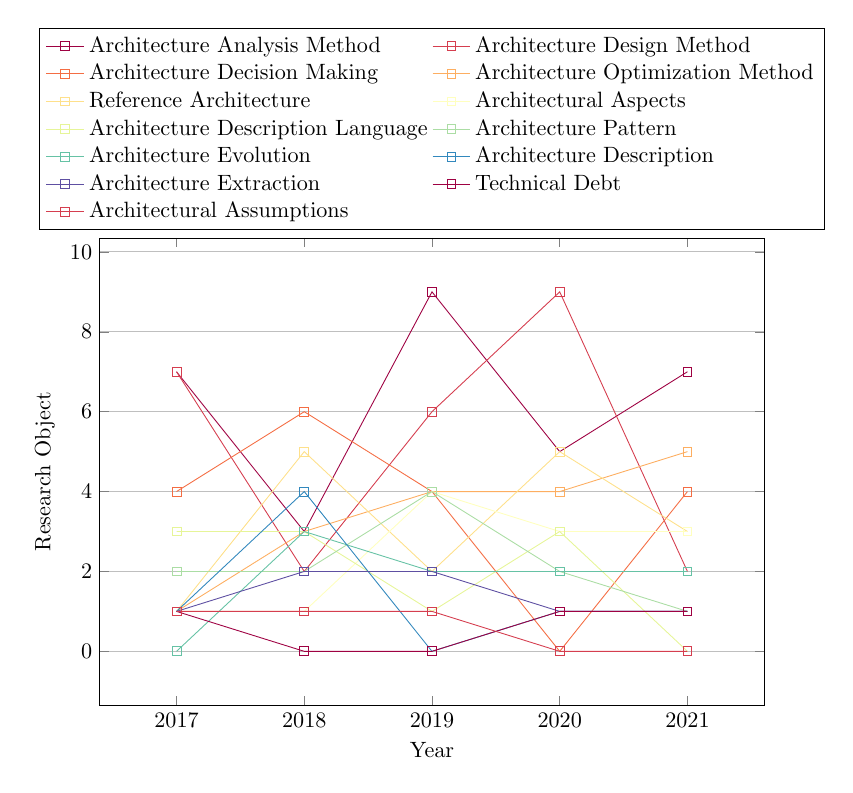
\begin{tikzpicture}[scale=0.8]
\
\begin{axis}[ width=\linewidth, height=9cm,
    cycle multi list=Spectral,
    every axis plot/.append style={draw,mark=square},
    %nodes near coords,nodes near coords style={color=black,font=\small},
    enlargelimits=0.15, 
    bar width=3.5em,
    legend style={at={(0.5,1.45)}, anchor=north,legend columns=2},
    legend cell align={left},
    ylabel={Research Object},ymajorgrids,ymin=0,
    %x tick label style={rotate=45,anchor=east},
    xtick={1,2,3,4,5}, xticklabels={2017,2018,2019,2020,2021},
    xlabel={Year}    
   ]
\addplot coordinates { (1,7)  (2,3)  (3,9)  (4,5)  (5,7)  };
\addplot coordinates { (1,7)  (2,2)  (3,6)  (4,9)  (5,2)  };
\addplot coordinates { (1,4)  (2,6)  (3,4)  (4,0)  (5,4)  };
\addplot coordinates { (1,1)  (2,3)  (3,4)  (4,4)  (5,5)  };
\addplot coordinates { (1,1)  (2,5)  (3,2)  (4,5)  (5,3)  };
\addplot coordinates { (1,1)  (2,1)  (3,4)  (4,3)  (5,3)  };
\addplot coordinates { (1,3)  (2,3)  (3,1)  (4,3)  (5,0)  };
\addplot coordinates { (1,2)  (2,2)  (3,4)  (4,2)  (5,1)  };
\addplot coordinates { (1,0)  (2,3)  (3,2)  (4,2)  (5,2)  };
\addplot coordinates { (1,1)  (2,4)  (3,0)  (4,1)  (5,1)  };
\addplot coordinates { (1,1)  (2,2)  (3,2)  (4,1)  (5,1)  };
\addplot coordinates { (1,1)  (2,0)  (3,0)  (4,1)  (5,1)  };
\addplot coordinates { (1,1)  (2,1)  (3,1)  (4,0)  (5,0)  };

\legend{Architecture Analysis Method,Architecture Design Method,Architecture Decision Making,Architecture Optimization Method,Reference Architecture,Architectural Aspects,Architecture Description Language,Architecture Pattern,Architecture Evolution,Architecture Description,Architecture Extraction,Technical Debt,Architectural Assumptions}
\end{axis}
\end{tikzpicture}
\end{center}
%\caption{Plot von Year je Research Object}
%\label{fig:plot_year_researchobject}
%\end{figure}



\section{Evaluation Methods}

%\subsection{Histogramm f\"ur Evaluation Method (188)}
%\begin{figure}
\begin{center}
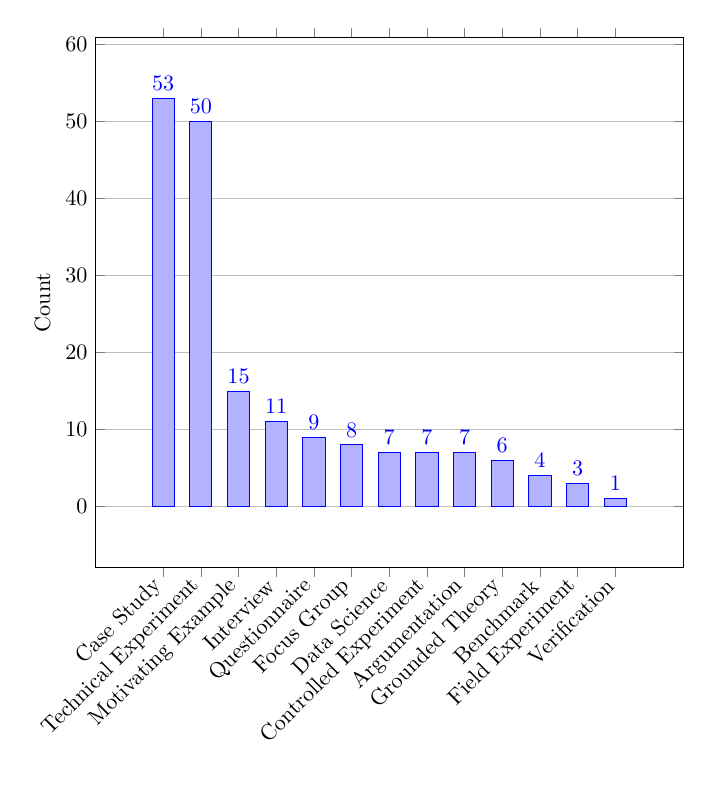
\begin{tikzpicture}[scale=.8]
\begin{axis}[ ybar, ymajorgrids, enlargelimits=0.15, legend style={at={(0.5,-0.15)}, anchor=north,legend columns=-1},
    width=.90\linewidth,height=10cm,
    nodes near coords, %nodes near coords align=below,
    ylabel={Count},ymin=0,
    x tick label style={rotate=45,anchor=east},
    xtick={1,2,3,4,5,6,7,8,9,10,11,12,13},
    xticklabels={Case Study,Technical Experiment,Motivating Example,Interview,Questionnaire,Focus Group,Data Science,Controlled Experiment,Argumentation,Grounded Theory,Benchmark,Field Experiment,Verification 
}
    %xlabel={Evaluation Method}    
    ]
  \addplot coordinates { (1,53)  (2,50)  (3,15)  (4,11)  (5,9)  (6,8)  (7,7)  (8,7)  (9,7)  (10,6)  (11,4)  (12,3)  (13,1)   };
\end{axis}
\end{tikzpicture}
\end{center}
%\caption{Histogramm f\"ur Evaluation Method (188)}
%\label{fig:histo_evaluationmethod}
%\end{figure}


%\subsection{Histogram von Year je Evaluation Method}
%\begin{figure}
\begin{center}
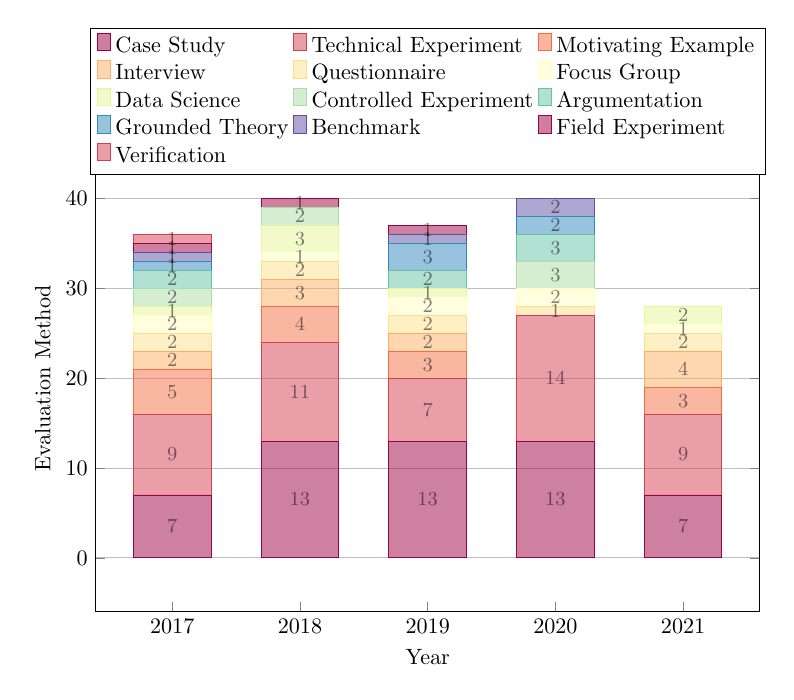
\begin{tikzpicture}[scale=0.8]
\
\begin{axis}[ width=\linewidth,height=9cm, ybar stacked,
    cycle multi list=Spectral,
    every axis plot/.append style={draw, fill, fill opacity=0.5},
    enlargelimits=0.15, 
    bar width=3.5em,
    nodes near coords, %nodes near coords align=below,
    nodes near coords style={color=black,font=\small},
    legend style={at={(0.5,1.25)}, anchor=north,legend columns=3},
    legend cell align={left},
    ylabel={Evaluation Method},ymajorgrids,ymin=0,
    %x tick label style={rotate=45,anchor=east},
    xtick={1,2,3,4,5}, xticklabels={2017,2018,2019,2020,2021},
    xlabel={Year}    
   ]
\addplot coordinates { (1,7)  (2,13)  (3,13)  (4,13)  (5,7)  };
\addplot coordinates { (1,9)  (2,11)  (3,7)  (4,14)  (5,9)  };
\addplot coordinates { (1,5)  (2,4)  (3,3)  (4,0)  (5,3)  };
\addplot coordinates { (1,2)  (2,3)  (3,2)  (4,0)  (5,4)  };
\addplot coordinates { (1,2)  (2,2)  (3,2)  (4,1)  (5,2)  };
\addplot coordinates { (1,2)  (2,1)  (3,2)  (4,2)  (5,1)  };
\addplot coordinates { (1,1)  (2,3)  (3,1)  (4,0)  (5,2)  };
\addplot coordinates { (1,2)  (2,2)  (3,0)  (4,3)  (5,0)  };
\addplot coordinates { (1,2)  (2,0)  (3,2)  (4,3)  (5,0)  };
\addplot coordinates { (1,1)  (2,0)  (3,3)  (4,2)  (5,0)  };
\addplot coordinates { (1,1)  (2,0)  (3,1)  (4,2)  (5,0)  };
\addplot coordinates { (1,1)  (2,1)  (3,1)  (4,0)  (5,0)  };
\addplot coordinates { (1,1)  (2,0)  (3,0)  (4,0)  (5,0)  };

\legend{Case Study,Technical Experiment,Motivating Example,Interview,Questionnaire,Focus Group,Data Science,Controlled Experiment,Argumentation,Grounded Theory,Benchmark,Field Experiment,Verification}
\end{axis}
\end{tikzpicture}
\end{center}
%\caption{Histogram von Year je Evaluation Method}
%\label{fig:chisto_year_evaluationmethod}
%\end{figure}


%\subsection{Kreisdiagramm f\"ur Evaluation Method (181)}
%\begin{figure}
\begin{center}
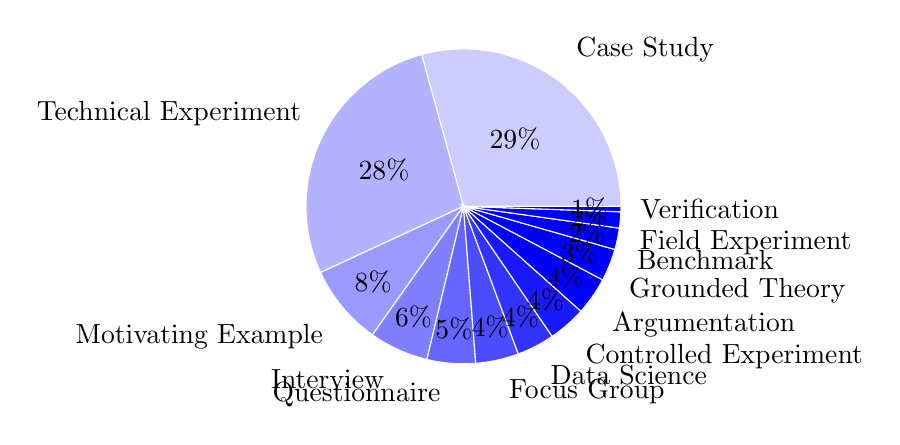
\begin{tikzpicture}[scale=2]
\pgfmathsetcounter{pied}{0}
\foreach \p/\q/\t/\c in {29/53/Case Study/blue!20, 28/50/Technical Experiment/blue!30, 8/15/Motivating Example/blue!40, 6/11/Interview/blue!50, 5/9/Questionnaire/blue!60, 4/8/Focus Group/blue!70, 4/7/Data Science/blue!80, 4/7/Controlled Experiment/blue!90, 4/7/Argumentation/blue!100, 3/6/Grounded Theory/blue!110, 2/4/Benchmark/blue!120, 2/3/Field Experiment/blue!130, 1/1/Verification/blue!140}
  {
    \setcounter{piec}{\value{pied}}
    \addtocounter{pied}{\q}
    \slice{\thepiec/181*360}
          {\thepied/181*360}
          {\p\%}{\t}{\c}
  }
\end{tikzpicture}
\end{center}
%\caption{Kreisdiagramm f\"ur Evaluation Method (181)}
%\label{fig:pie_evaluationmethod}
%\end{figure}


%\subsection{Portfolio f\"ur Year und Evaluation Method (Gr\"o\ss{}e entspricht der Anzahl)}
%\begin{figure}
\begin{center}
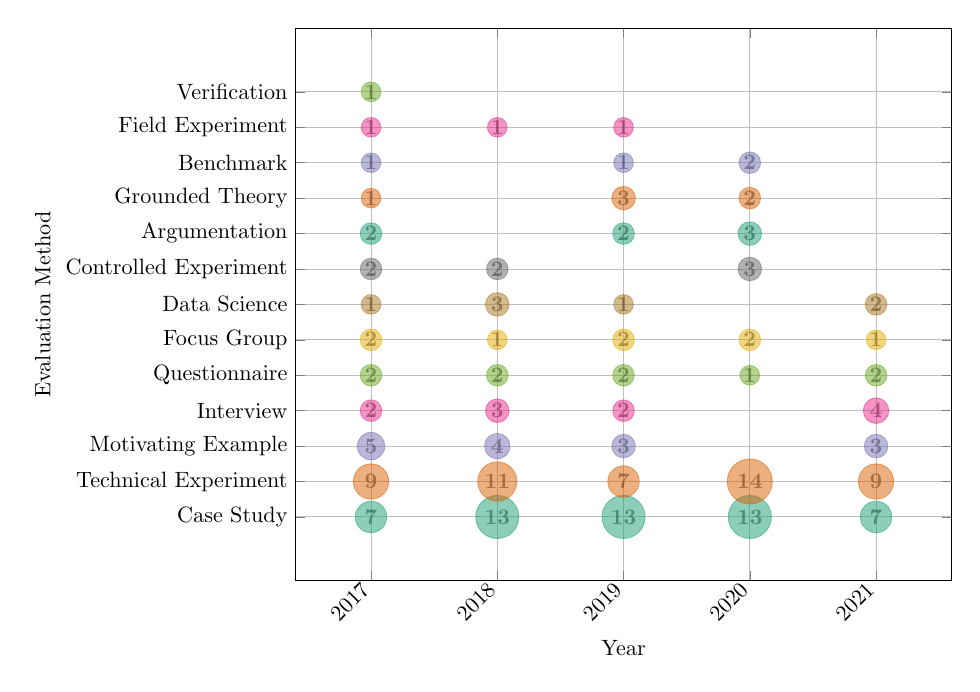
\begin{tikzpicture}[scale=.8]
\pgfplotsset{cycle list/Dark2}
\begin{axis}[width=.99\linewidth,
    enlargelimits=0.15,
    x tick label style={rotate=45,anchor=east},
    xtick={0,1,2,3,4}, xticklabels={2017,2018,2019,2020,2021},
    xlabel={Year},
    ytick={0,1,2,3,4,5,6,7,8,9,10,11,12}, yticklabels={Case Study,Technical Experiment,Motivating Example,Interview,Questionnaire,Focus Group,Data Science,Controlled Experiment,Argumentation,Grounded Theory,Benchmark,Field Experiment,Verification},
    ylabel={Evaluation Method},
    grid=both,
    scatter,scatter src=y,
    scatter/classes={0={draw=Dark2-A,fill=Dark2-A}, 1={draw=Dark2-B,fill=Dark2-B}, 2={draw=Dark2-C,fill=Dark2-C}, 3={draw=Dark2-D,fill=Dark2-D}, 4={draw=Dark2-E,fill=Dark2-E}, 5={draw=Dark2-F,fill=Dark2-F}, 6={draw=Dark2-G,fill=Dark2-G}, 7={draw=Dark2-H,fill=Dark2-H}, 8={draw=Dark2-A,fill=Dark2-A}, 9={draw=Dark2-B,fill=Dark2-B}, 10={draw=Dark2-C,fill=Dark2-C}, 11={draw=Dark2-D,fill=Dark2-D}, 12={draw=Dark2-E,fill=Dark2-E}}
]

\addplot+[mark=*,mark size=7.094,opacity=0.5,text=black] coordinates { (0,0) } node[text=black,font=\bfseries] {7};
\addplot+[mark=*,mark size=7.978,opacity=0.5,text=black] coordinates { (0,1) } node[text=black,font=\bfseries] {9};
\addplot+[mark=*,mark size=6.210,opacity=0.5,text=black] coordinates { (0,2) } node[text=black,font=\bfseries] {5};
\addplot+[mark=*,mark size=4.884,opacity=0.5,text=black] coordinates { (0,3) } node[text=black,font=\bfseries] {2};
\addplot+[mark=*,mark size=4.884,opacity=0.5,text=black] coordinates { (0,4) } node[text=black,font=\bfseries] {2};
\addplot+[mark=*,mark size=4.884,opacity=0.5,text=black] coordinates { (0,5) } node[text=black,font=\bfseries] {2};
\addplot+[mark=*,mark size=4.442,opacity=0.5,text=black] coordinates { (0,6) } node[text=black,font=\bfseries] {1};
\addplot+[mark=*,mark size=4.884,opacity=0.5,text=black] coordinates { (0,7) } node[text=black,font=\bfseries] {2};
\addplot+[mark=*,mark size=4.884,opacity=0.5,text=black] coordinates { (0,8) } node[text=black,font=\bfseries] {2};
\addplot+[mark=*,mark size=4.442,opacity=0.5,text=black] coordinates { (0,9) } node[text=black,font=\bfseries] {1};
\addplot+[mark=*,mark size=4.442,opacity=0.5,text=black] coordinates { (0,10) } node[text=black,font=\bfseries] {1};
\addplot+[mark=*,mark size=4.442,opacity=0.5,text=black] coordinates { (0,11) } node[text=black,font=\bfseries] {1};
\addplot+[mark=*,mark size=4.442,opacity=0.5,text=black] coordinates { (0,12) } node[text=black,font=\bfseries] {1};
\addplot+[mark=*,mark size=9.746,opacity=0.5,text=black] coordinates { (1,0) } node[text=black,font=\bfseries] {13};
\addplot+[mark=*,mark size=8.862,opacity=0.5,text=black] coordinates { (1,1) } node[text=black,font=\bfseries] {11};
\addplot+[mark=*,mark size=5.768,opacity=0.5,text=black] coordinates { (1,2) } node[text=black,font=\bfseries] {4};
\addplot+[mark=*,mark size=5.326,opacity=0.5,text=black] coordinates { (1,3) } node[text=black,font=\bfseries] {3};
\addplot+[mark=*,mark size=4.884,opacity=0.5,text=black] coordinates { (1,4) } node[text=black,font=\bfseries] {2};
\addplot+[mark=*,mark size=4.442,opacity=0.5,text=black] coordinates { (1,5) } node[text=black,font=\bfseries] {1};
\addplot+[mark=*,mark size=5.326,opacity=0.5,text=black] coordinates { (1,6) } node[text=black,font=\bfseries] {3};
\addplot+[mark=*,mark size=4.884,opacity=0.5,text=black] coordinates { (1,7) } node[text=black,font=\bfseries] {2};
\addplot+[mark=*,mark size=4.442,opacity=0.5,text=black] coordinates { (1,11) } node[text=black,font=\bfseries] {1};
\addplot+[mark=*,mark size=9.746,opacity=0.5,text=black] coordinates { (2,0) } node[text=black,font=\bfseries] {13};
\addplot+[mark=*,mark size=7.094,opacity=0.5,text=black] coordinates { (2,1) } node[text=black,font=\bfseries] {7};
\addplot+[mark=*,mark size=5.326,opacity=0.5,text=black] coordinates { (2,2) } node[text=black,font=\bfseries] {3};
\addplot+[mark=*,mark size=4.884,opacity=0.5,text=black] coordinates { (2,3) } node[text=black,font=\bfseries] {2};
\addplot+[mark=*,mark size=4.884,opacity=0.5,text=black] coordinates { (2,4) } node[text=black,font=\bfseries] {2};
\addplot+[mark=*,mark size=4.884,opacity=0.5,text=black] coordinates { (2,5) } node[text=black,font=\bfseries] {2};
\addplot+[mark=*,mark size=4.442,opacity=0.5,text=black] coordinates { (2,6) } node[text=black,font=\bfseries] {1};
\addplot+[mark=*,mark size=4.884,opacity=0.5,text=black] coordinates { (2,8) } node[text=black,font=\bfseries] {2};
\addplot+[mark=*,mark size=5.326,opacity=0.5,text=black] coordinates { (2,9) } node[text=black,font=\bfseries] {3};
\addplot+[mark=*,mark size=4.442,opacity=0.5,text=black] coordinates { (2,10) } node[text=black,font=\bfseries] {1};
\addplot+[mark=*,mark size=4.442,opacity=0.5,text=black] coordinates { (2,11) } node[text=black,font=\bfseries] {1};
\addplot+[mark=*,mark size=9.746,opacity=0.5,text=black] coordinates { (3,0) } node[text=black,font=\bfseries] {13};
\addplot+[mark=*,mark size=10.188,opacity=0.5,text=black] coordinates { (3,1) } node[text=black,font=\bfseries] {14};
\addplot+[mark=*,mark size=4.442,opacity=0.5,text=black] coordinates { (3,4) } node[text=black,font=\bfseries] {1};
\addplot+[mark=*,mark size=4.884,opacity=0.5,text=black] coordinates { (3,5) } node[text=black,font=\bfseries] {2};
\addplot+[mark=*,mark size=5.326,opacity=0.5,text=black] coordinates { (3,7) } node[text=black,font=\bfseries] {3};
\addplot+[mark=*,mark size=5.326,opacity=0.5,text=black] coordinates { (3,8) } node[text=black,font=\bfseries] {3};
\addplot+[mark=*,mark size=4.884,opacity=0.5,text=black] coordinates { (3,9) } node[text=black,font=\bfseries] {2};
\addplot+[mark=*,mark size=4.884,opacity=0.5,text=black] coordinates { (3,10) } node[text=black,font=\bfseries] {2};
\addplot+[mark=*,mark size=7.094,opacity=0.5,text=black] coordinates { (4,0) } node[text=black,font=\bfseries] {7};
\addplot+[mark=*,mark size=7.978,opacity=0.5,text=black] coordinates { (4,1) } node[text=black,font=\bfseries] {9};
\addplot+[mark=*,mark size=5.326,opacity=0.5,text=black] coordinates { (4,2) } node[text=black,font=\bfseries] {3};
\addplot+[mark=*,mark size=5.768,opacity=0.5,text=black] coordinates { (4,3) } node[text=black,font=\bfseries] {4};
\addplot+[mark=*,mark size=4.884,opacity=0.5,text=black] coordinates { (4,4) } node[text=black,font=\bfseries] {2};
\addplot+[mark=*,mark size=4.442,opacity=0.5,text=black] coordinates { (4,5) } node[text=black,font=\bfseries] {1};
\addplot+[mark=*,mark size=4.884,opacity=0.5,text=black] coordinates { (4,6) } node[text=black,font=\bfseries] {2};


\end{axis}
\end{tikzpicture}
\end{center}
%\caption{Portfolio f\"ur Year und Evaluation Method (Gr\"o\ss{}e entspricht der Anzahl)}\label{fig:port_year_evaluationmethod}
%\end{figure}


%\subsection{Plot von Year je Evaluation Method}
%\begin{figure}
\begin{center}
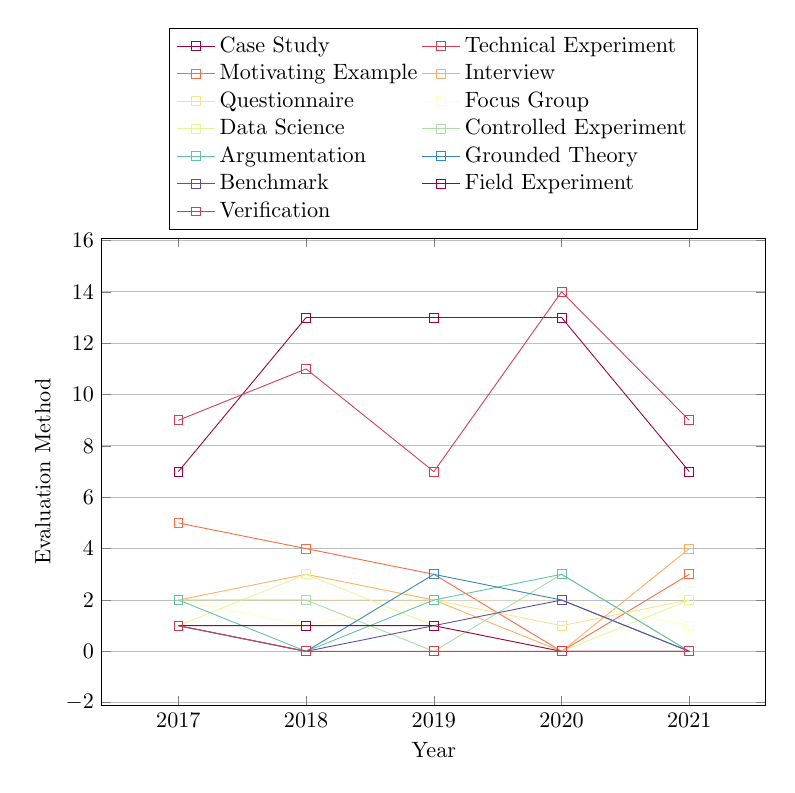
\begin{tikzpicture}[scale=0.8]
\
\begin{axis}[ width=\linewidth, height=9cm,
    cycle multi list=Spectral,
    every axis plot/.append style={draw,mark=square},
    %nodes near coords,nodes near coords style={color=black,font=\small},
    enlargelimits=0.15, 
    bar width=3.5em,
    legend style={at={(0.5,1.45)}, anchor=north,legend columns=2},
    legend cell align={left},
    ylabel={Evaluation Method}, ymajorgrids,ymin=0,
    %x tick label style={rotate=45,anchor=east},
    xtick={1,2,3,4,5}, xticklabels={2017,2018,2019,2020,2021},
    xlabel={Year}
   ]
\addplot coordinates { (1,7)  (2,13)  (3,13)  (4,13)  (5,7)  };
\addplot coordinates { (1,9)  (2,11)  (3,7)  (4,14)  (5,9)  };
\addplot coordinates { (1,5)  (2,4)  (3,3)  (4,0)  (5,3)  };
\addplot coordinates { (1,2)  (2,3)  (3,2)  (4,0)  (5,4)  };
\addplot coordinates { (1,2)  (2,2)  (3,2)  (4,1)  (5,2)  };
\addplot coordinates { (1,2)  (2,1)  (3,2)  (4,2)  (5,1)  };
\addplot coordinates { (1,1)  (2,3)  (3,1)  (4,0)  (5,2)  };
\addplot coordinates { (1,2)  (2,2)  (3,0)  (4,3)  (5,0)  };
\addplot coordinates { (1,2)  (2,0)  (3,2)  (4,3)  (5,0)  };
\addplot coordinates { (1,1)  (2,0)  (3,3)  (4,2)  (5,0)  };
\addplot coordinates { (1,1)  (2,0)  (3,1)  (4,2)  (5,0)  };
\addplot coordinates { (1,1)  (2,1)  (3,1)  (4,0)  (5,0)  };
\addplot coordinates { (1,1)  (2,0)  (3,0)  (4,0)  (5,0)  };

\legend{Case Study,Technical Experiment,Motivating Example,Interview,Questionnaire,Focus Group,Data Science,Controlled Experiment,Argumentation,Grounded Theory,Benchmark,Field Experiment,Verification}
\end{axis}
\end{tikzpicture}
\end{center}
%\caption{Plot von Year je Evaluation Method}
%\label{fig:plot_year_evaluationmethod}
%\end{figure}



\section{Replication Package}

%\subsection{Histogramm f\"ur Tool Support (153)}
%\begin{figure}
\begin{center}
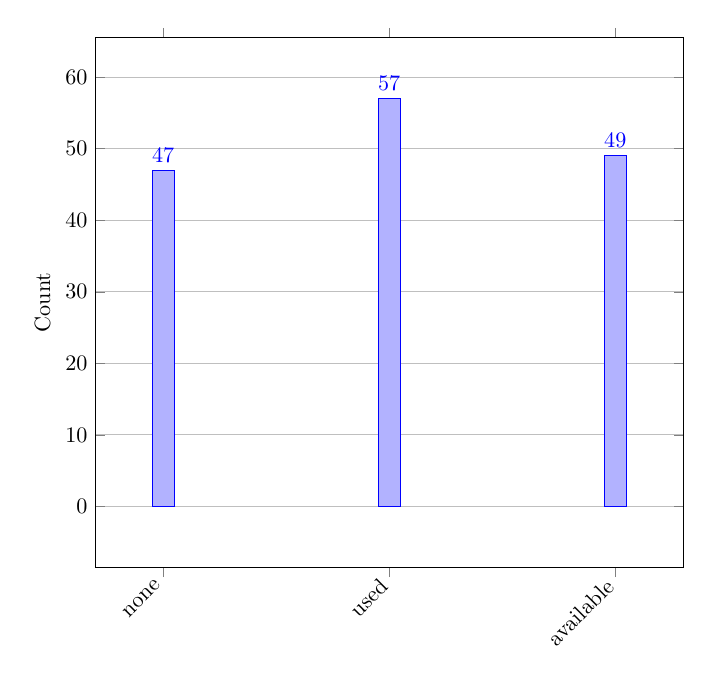
\begin{tikzpicture}[scale=.8]
\begin{axis}[ ybar, ymajorgrids, enlargelimits=0.15, legend style={at={(0.5,-0.15)}, anchor=north,legend columns=-1},
    width=.90\linewidth,height=10cm,
    nodes near coords, %nodes near coords align=below,
    ylabel={Count}, ymin=0,
    x tick label style={rotate=45,anchor=east},
    xtick={1,2,3},
    xticklabels={none,used,available
}
    %xlabel={Tool Support}    
    ]
  \addplot coordinates { (1,47)  (2,57)  (3,49)   };
\end{axis}
\end{tikzpicture}
\end{center}
%\caption{Histogramm f\"ur Tool Support (153)}
%\label{fig:histo_toolsupport}
%\end{figure}


%\subsection{Pie chart for Tool Support (153)}
%\begin{figure}
\begin{center}
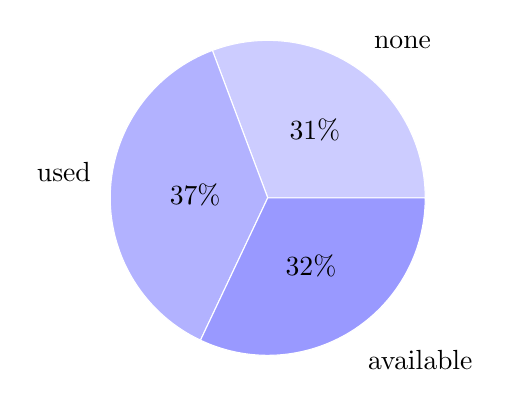
\begin{tikzpicture}[scale=2]
\pgfmathsetcounter{pief}{0}
\foreach \p/\q/\t/\c in {31/47/none/blue!20, 37/57/used/blue!30, 32/49/available/blue!40}
  {
    \setcounter{piee}{\value{pief}}
    \addtocounter{pief}{\q}
    \slice{\thepiee/153*360}
          {\thepief/153*360}
          {\p\%}{\t}{\c}
  }
\end{tikzpicture}

\textbf{Pie chart for Tool Support (153)}
\end{center}
%\caption{Pie chart for Tool Support (153)}
%\label{fig:pie_toolsupport}
%\end{figure}


%\subsection{Histogram von Year je Tool Support}
%\begin{figure}
\begin{center}
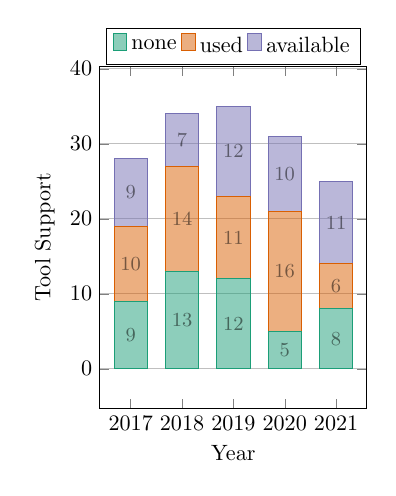
\begin{tikzpicture}[scale=0.8]
\pgfplotsset{cycle list/Dark2}
\begin{axis}[ width=.48\linewidth,height=7cm, ybar stacked,
    every axis plot/.append style={draw, fill, fill opacity=0.5},
    enlargelimits=0.15, 
    bar width=1.5em,
    nodes near coords, %nodes near coords align=below,
    nodes near coords style={color=black,font=\small},
    legend style={at={(0.5,1.115)}, anchor=north,legend columns=3},
    legend cell align={left},
    ylabel={Tool Support},ymajorgrids,ymin=0,
    %x tick label style={rotate=45,anchor=east},
    ymin=0,
    xtick={1,2,3,4,5}, xticklabels={2017,2018,2019,2020,2021},
    xlabel={Year},
    cycle multi list=Dark2    
   ]
\addplot coordinates { (1,9)  (2,13)  (3,12)  (4,5)  (5,8)  };
\addplot coordinates { (1,10)  (2,14)  (3,11)  (4,16)  (5,6)  };
\addplot coordinates { (1,9)  (2,7)  (3,12)  (4,10)  (5,11)  };

\legend{none,used,available}
\end{axis}
\end{tikzpicture}
\end{center}
%\caption{Histogram von Year je Tool Support}
%\label{fig:chisto_year_toolsupport}
%\end{figure}


%\subsection{Portfolio f\"ur Year und Tool Support (Gr\"o\ss{}e entspricht der Anzahl)}
%\begin{figure}
\begin{center}
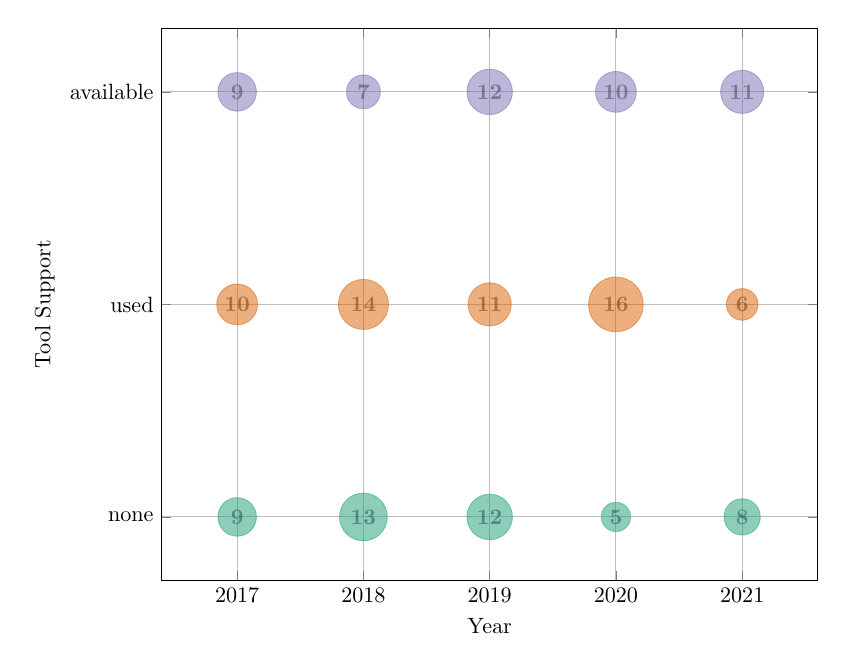
\begin{tikzpicture}[scale=.8]
\pgfplotsset{cycle list/Dark2}
\begin{axis}[width=.99\linewidth,
    enlargelimits=0.15,
    %x tick label style={rotate=45,anchor=east},
    xtick={0,1,2,3,4}, xticklabels={2017,2018,2019,2020,2021},
    xlabel={Year},
    ytick={0,1,2}, yticklabels={none,used,available},
    ylabel={Tool Support},
    grid=both,
    scatter,scatter src=y,
    scatter/classes={0={draw=Dark2-A,fill=Dark2-A}, 1={draw=Dark2-B,fill=Dark2-B}, 2={draw=Dark2-C,fill=Dark2-C}}
]

\addplot+[mark=*,mark size=8.706,opacity=0.5,text=black] coordinates { (0,0) } node[text=black,font=\bfseries] {9};
\addplot+[mark=*,mark size=9.229,opacity=0.5,text=black] coordinates { (0,1) } node[text=black,font=\bfseries] {10};
\addplot+[mark=*,mark size=8.706,opacity=0.5,text=black] coordinates { (0,2) } node[text=black,font=\bfseries] {9};
\addplot+[mark=*,mark size=10.797,opacity=0.5,text=black] coordinates { (1,0) } node[text=black,font=\bfseries] {13};
\addplot+[mark=*,mark size=11.320,opacity=0.5,text=black] coordinates { (1,1) } node[text=black,font=\bfseries] {14};
\addplot+[mark=*,mark size=7.660,opacity=0.5,text=black] coordinates { (1,2) } node[text=black,font=\bfseries] {7};
\addplot+[mark=*,mark size=10.275,opacity=0.5,text=black] coordinates { (2,0) } node[text=black,font=\bfseries] {12};
\addplot+[mark=*,mark size=9.752,opacity=0.5,text=black] coordinates { (2,1) } node[text=black,font=\bfseries] {11};
\addplot+[mark=*,mark size=10.275,opacity=0.5,text=black] coordinates { (2,2) } node[text=black,font=\bfseries] {12};
\addplot+[mark=*,mark size=6.614,opacity=0.5,text=black] coordinates { (3,0) } node[text=black,font=\bfseries] {5};
\addplot+[mark=*,mark size=12.366,opacity=0.5,text=black] coordinates { (3,1) } node[text=black,font=\bfseries] {16};
\addplot+[mark=*,mark size=9.229,opacity=0.5,text=black] coordinates { (3,2) } node[text=black,font=\bfseries] {10};
\addplot+[mark=*,mark size=8.183,opacity=0.5,text=black] coordinates { (4,0) } node[text=black,font=\bfseries] {8};
\addplot+[mark=*,mark size=7.137,opacity=0.5,text=black] coordinates { (4,1) } node[text=black,font=\bfseries] {6};
\addplot+[mark=*,mark size=9.752,opacity=0.5,text=black] coordinates { (4,2) } node[text=black,font=\bfseries] {11};


\end{axis}
\end{tikzpicture}
\end{center}
%\caption{Portfolio f\"ur Year und Tool Support (Gr\"o\ss{}e entspricht der Anzahl)}\label{fig:port_year_toolsupport}
%\end{figure}


%\subsection{Plot von Year je Tool Support}
%\begin{figure}
\begin{center}
\pgfplotsset{cycle list/Dark2}
\begin{tikzpicture}[scale=0.8]
\
\begin{axis}[ width=\linewidth, height=9cm,
    every axis plot/.append style={draw,mark=square},
    %nodes near coords,nodes near coords style={color=black,font=\small},
    enlargelimits=0.15, 
    bar width=3.5em,
    legend style={at={(0.5,1.1)}, anchor=north,legend columns=3},
    legend cell align={left},
    ylabel={Tool Support},ymajorgrids,ymin=0,
    %x tick label style={rotate=45,anchor=east},
    xtick={1,2,3,4,5}, xticklabels={2017,2018,2019,2020,2021},
    xlabel={Year},
    cycle multi list=Dark2
   ]
\addplot coordinates { (1,9)  (2,13)  (3,12)  (4,5)  (5,8)  };
\addplot coordinates { (1,10)  (2,14)  (3,11)  (4,16)  (5,6)  };
\addplot coordinates { (1,9)  (2,7)  (3,12)  (4,10)  (5,11)  };

\legend{none,used,available}
\end{axis}
\end{tikzpicture}
\end{center}
%\caption{Plot von Year je Tool Support}
%\label{fig:plot_year_toolsupport}
%\end{figure}



%\subsection{Histogramm f\"ur Input Data (153)}
%\begin{figure}
\begin{center}
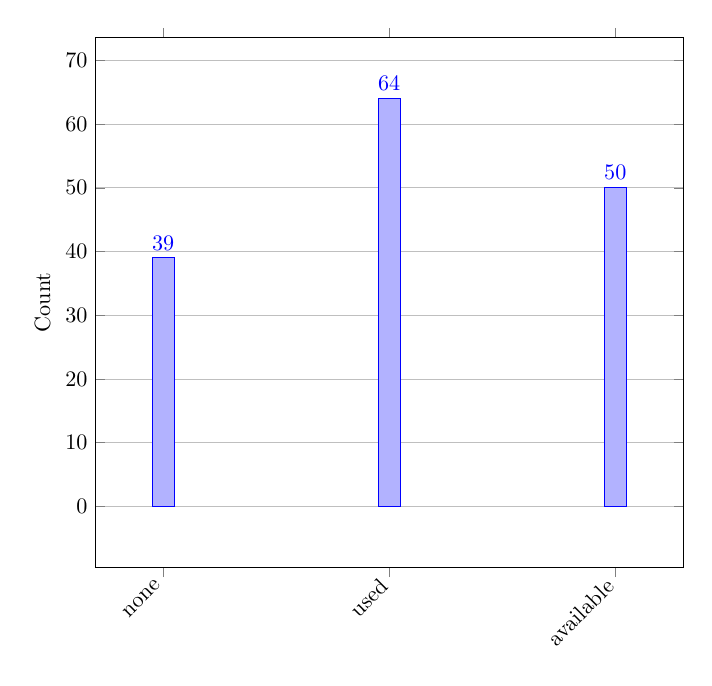
\begin{tikzpicture}[scale=.8]
\begin{axis}[ ybar, ymajorgrids, enlargelimits=0.15, legend style={at={(0.5,-0.15)}, anchor=north,legend columns=-1},
    width=.90\linewidth,height=10cm,
    nodes near coords, %nodes near coords align=below,
    ylabel={Count}, ymin=0,
    x tick label style={rotate=45,anchor=east},
    xtick={1,2,3},
    xticklabels={none,used,available
}
    %xlabel={Input Data}    
    ]
  \addplot coordinates { (1,39)  (2,64)  (3,50)   };
\end{axis}
\end{tikzpicture}
\end{center}
%\caption{Histogramm f\"ur Input Data (153)}
%\label{fig:histo_inputdata}
%\end{figure}


%\subsection{Pie chart for Input Data (153)}
%\begin{figure}
\begin{center}
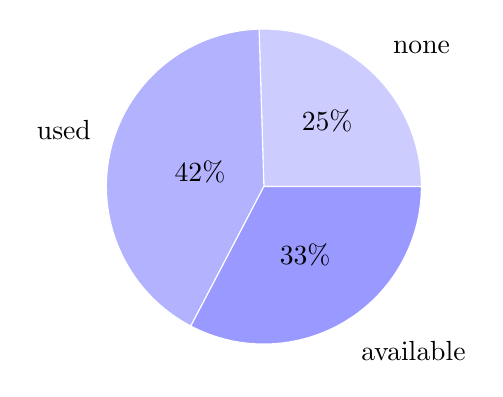
\begin{tikzpicture}[scale=2]
\pgfmathsetcounter{pief}{0}
\foreach \p/\q/\t/\c in {25/39/none/blue!20, 42/64/used/blue!30, 33/50/available/blue!40}
  {
    \setcounter{piee}{\value{pief}}
    \addtocounter{pief}{\q}
    \slice{\thepiee/153*360}
          {\thepief/153*360}
          {\p\%}{\t}{\c}
  }
\end{tikzpicture}

\textbf{Pie chart for Input Data (153)}
\end{center}
%\caption{Pie chart for Input Data (153)}
%\label{fig:pie_inputdata}
%\end{figure}


%\subsection{Histogram von Year je Input Data}
%\begin{figure}
\begin{center}
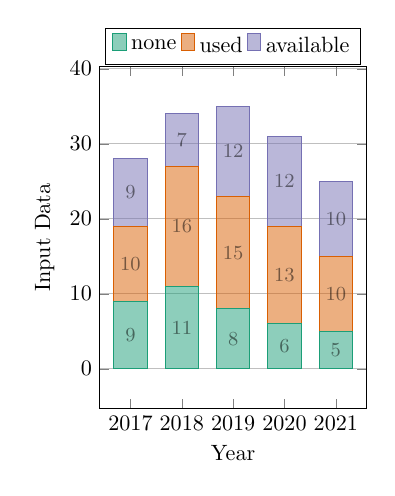
\begin{tikzpicture}[scale=0.8]
\pgfplotsset{cycle list/Dark2}
\begin{axis}[ width=.48\linewidth,height=7cm, ybar stacked,
    every axis plot/.append style={draw, fill, fill opacity=0.5},
    enlargelimits=0.15, 
    bar width=1.5em,
    nodes near coords, %nodes near coords align=below,
    nodes near coords style={color=black,font=\small},
    legend style={at={(0.5,1.115)}, anchor=north,legend columns=3},
    legend cell align={left},
    ylabel={Input Data},ymajorgrids,ymin=0,
    %x tick label style={rotate=45,anchor=east},
    ymin=0,
    xtick={1,2,3,4,5}, xticklabels={2017,2018,2019,2020,2021},
    xlabel={Year},
    cycle multi list=Dark2    
   ]
\addplot coordinates { (1,9)  (2,11)  (3,8)  (4,6)  (5,5)  };
\addplot coordinates { (1,10)  (2,16)  (3,15)  (4,13)  (5,10)  };
\addplot coordinates { (1,9)  (2,7)  (3,12)  (4,12)  (5,10)  };

\legend{none,used,available}
\end{axis}
\end{tikzpicture}
\end{center}
%\caption{Histogram von Year je Input Data}
%\label{fig:chisto_year_inputdata}
%\end{figure}


%\subsection{Portfolio f\"ur Year und Input Data (Gr\"o\ss{}e entspricht der Anzahl)}
%\begin{figure}
\begin{center}
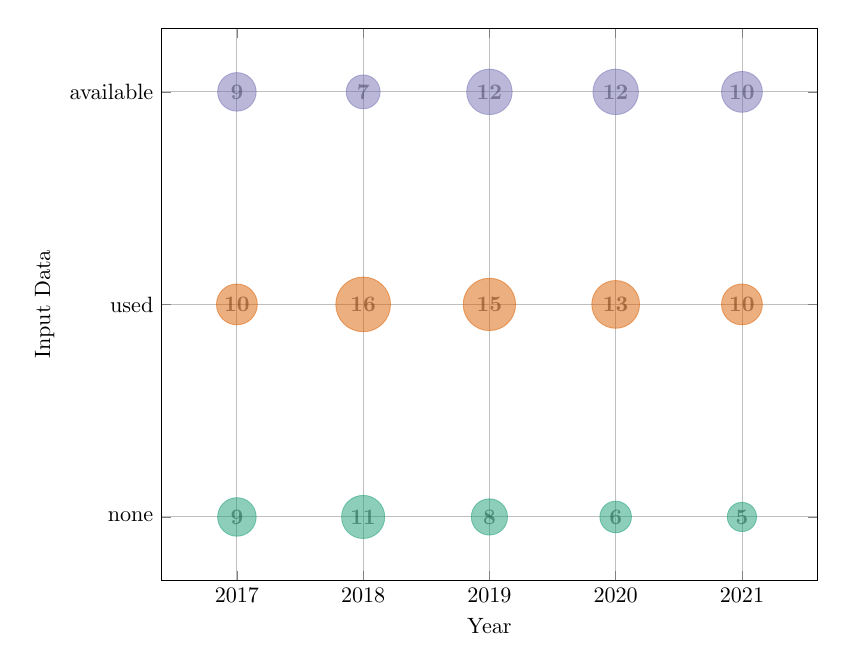
\begin{tikzpicture}[scale=.8]
\pgfplotsset{cycle list/Dark2}
\begin{axis}[width=.99\linewidth,
    enlargelimits=0.15,
    %x tick label style={rotate=45,anchor=east},
    xtick={0,1,2,3,4}, xticklabels={2017,2018,2019,2020,2021},
    xlabel={Year},
    ytick={0,1,2}, yticklabels={none,used,available},
    ylabel={Input Data},
    grid=both,
    scatter,scatter src=y,
    scatter/classes={0={draw=Dark2-A,fill=Dark2-A}, 1={draw=Dark2-B,fill=Dark2-B}, 2={draw=Dark2-C,fill=Dark2-C}}
]

\addplot+[mark=*,mark size=8.706,opacity=0.5,text=black] coordinates { (0,0) } node[text=black,font=\bfseries] {9};
\addplot+[mark=*,mark size=9.229,opacity=0.5,text=black] coordinates { (0,1) } node[text=black,font=\bfseries] {10};
\addplot+[mark=*,mark size=8.706,opacity=0.5,text=black] coordinates { (0,2) } node[text=black,font=\bfseries] {9};
\addplot+[mark=*,mark size=9.752,opacity=0.5,text=black] coordinates { (1,0) } node[text=black,font=\bfseries] {11};
\addplot+[mark=*,mark size=12.366,opacity=0.5,text=black] coordinates { (1,1) } node[text=black,font=\bfseries] {16};
\addplot+[mark=*,mark size=7.660,opacity=0.5,text=black] coordinates { (1,2) } node[text=black,font=\bfseries] {7};
\addplot+[mark=*,mark size=8.183,opacity=0.5,text=black] coordinates { (2,0) } node[text=black,font=\bfseries] {8};
\addplot+[mark=*,mark size=11.843,opacity=0.5,text=black] coordinates { (2,1) } node[text=black,font=\bfseries] {15};
\addplot+[mark=*,mark size=10.275,opacity=0.5,text=black] coordinates { (2,2) } node[text=black,font=\bfseries] {12};
\addplot+[mark=*,mark size=7.137,opacity=0.5,text=black] coordinates { (3,0) } node[text=black,font=\bfseries] {6};
\addplot+[mark=*,mark size=10.797,opacity=0.5,text=black] coordinates { (3,1) } node[text=black,font=\bfseries] {13};
\addplot+[mark=*,mark size=10.275,opacity=0.5,text=black] coordinates { (3,2) } node[text=black,font=\bfseries] {12};
\addplot+[mark=*,mark size=6.614,opacity=0.5,text=black] coordinates { (4,0) } node[text=black,font=\bfseries] {5};
\addplot+[mark=*,mark size=9.229,opacity=0.5,text=black] coordinates { (4,1) } node[text=black,font=\bfseries] {10};
\addplot+[mark=*,mark size=9.229,opacity=0.5,text=black] coordinates { (4,2) } node[text=black,font=\bfseries] {10};


\end{axis}
\end{tikzpicture}
\end{center}
%\caption{Portfolio f\"ur Year und Input Data (Gr\"o\ss{}e entspricht der Anzahl)}\label{fig:port_year_inputdata}
%\end{figure}


%\subsection{Plot von Year je Input Data}
%\begin{figure}
\begin{center}
\pgfplotsset{cycle list/Dark2}
\begin{tikzpicture}[scale=0.8]
\
\begin{axis}[ width=\linewidth, height=9cm,
    every axis plot/.append style={draw,mark=square},
    %nodes near coords,nodes near coords style={color=black,font=\small},
    enlargelimits=0.15, 
    bar width=3.5em,
    legend style={at={(0.5,1.1)}, anchor=north,legend columns=3},
    legend cell align={left},
    ylabel={Input Data},ymajorgrids,ymin=0,
    %x tick label style={rotate=45,anchor=east},
    xtick={1,2,3,4,5}, xticklabels={2017,2018,2019,2020,2021},
    xlabel={Year},
    cycle multi list=Dark2
   ]
\addplot coordinates { (1,9)  (2,11)  (3,8)  (4,6)  (5,5)  };
\addplot coordinates { (1,10)  (2,16)  (3,15)  (4,13)  (5,10)  };
\addplot coordinates { (1,9)  (2,7)  (3,12)  (4,12)  (5,10)  };

\legend{none,used,available}
\end{axis}
\end{tikzpicture}
\end{center}
%\caption{Plot von Year je Input Data}
%\label{fig:plot_year_inputdata}
%\end{figure}



%\subsection{Histogramm f\"ur Replication Package (153)}
%\begin{figure}
\begin{center}
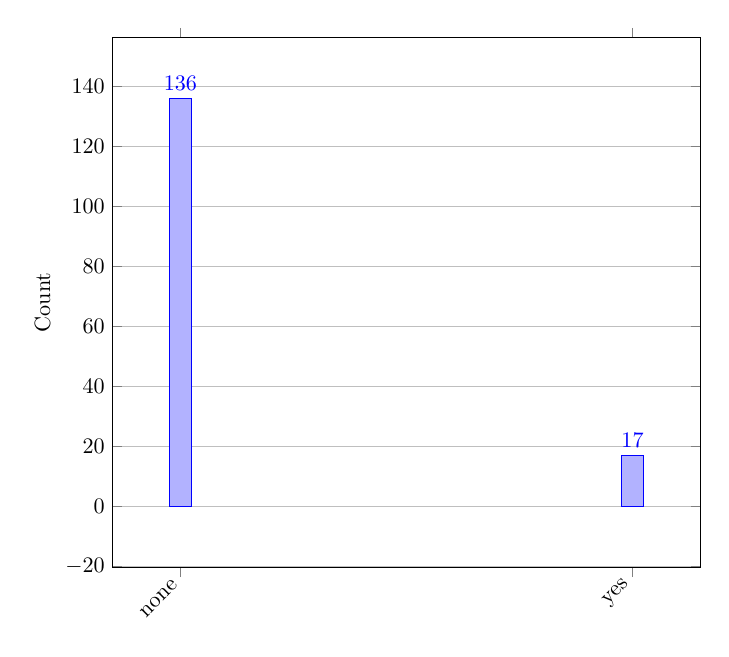
\begin{tikzpicture}[scale=.8]
\begin{axis}[ ybar, ymajorgrids, enlargelimits=0.15, legend style={at={(0.5,-0.15)}, anchor=north,legend columns=-1},
    width=.90\linewidth,height=10cm,
    nodes near coords, %nodes near coords align=below,
    ylabel={Count}, ymin=0,
    x tick label style={rotate=45,anchor=east},
    xtick={1,2},
    xticklabels={none,yes
}
    %xlabel={Replication Package}    
    ]
  \addplot coordinates { (1,136)  (2,17)   };
\end{axis}
\end{tikzpicture}
\end{center}
%\caption{Histogramm f\"ur Replication Package (153)}
%\label{fig:histo_replicationpackage}
%\end{figure}


%\subsection{Pie chart for Replication Package (153)}
%\begin{figure}
\begin{center}
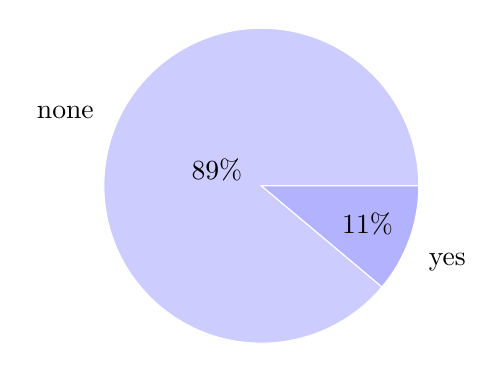
\begin{tikzpicture}[scale=2]
\pgfmathsetcounter{pief}{0}
\foreach \p/\q/\t/\c in {89/136/none/blue!20, 11/17/yes/blue!30}
  {
    \setcounter{piee}{\value{pief}}
    \addtocounter{pief}{\q}
    \slice{\thepiee/153*360}
          {\thepief/153*360}
          {\p\%}{\t}{\c}
  }
\end{tikzpicture}

\textbf{Pie chart for Replication Package (153)}
\end{center}
%\caption{Pie chart for Replication Package (153)}
%\label{fig:pie_replicationpackage}
%\end{figure}


%\subsection{Histogram von Year je Replication Package}
%\begin{figure}
\begin{center}
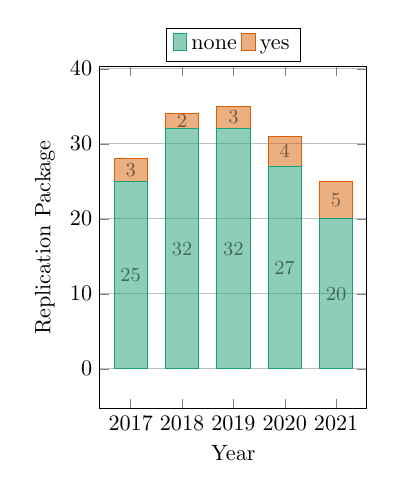
\begin{tikzpicture}[scale=0.8]
\pgfplotsset{cycle list/Dark2}
\begin{axis}[ width=.48\linewidth,height=7cm, ybar stacked,
    every axis plot/.append style={draw, fill, fill opacity=0.5},
    enlargelimits=0.15, 
    bar width=1.5em,
    nodes near coords, %nodes near coords align=below,
    nodes near coords style={color=black,font=\small},
    legend style={at={(0.5,1.115)}, anchor=north,legend columns=3},
    legend cell align={left},
    ylabel={Replication Package},ymajorgrids,ymin=0,
    %x tick label style={rotate=45,anchor=east},
    ymin=0,
    xtick={1,2,3,4,5}, xticklabels={2017,2018,2019,2020,2021},
    xlabel={Year},
    cycle multi list=Dark2    
   ]
\addplot coordinates { (1,25)  (2,32)  (3,32)  (4,27)  (5,20)  };
\addplot coordinates { (1,3)  (2,2)  (3,3)  (4,4)  (5,5)  };

\legend{none,yes}
\end{axis}
\end{tikzpicture}
\end{center}
%\caption{Histogram von Year je Replication Package}
%\label{fig:chisto_year_replicationpackage}
%\end{figure}


%\subsection{Portfolio f\"ur Year und Replication Package (Gr\"o\ss{}e entspricht der Anzahl)}
%\begin{figure}
\begin{center}
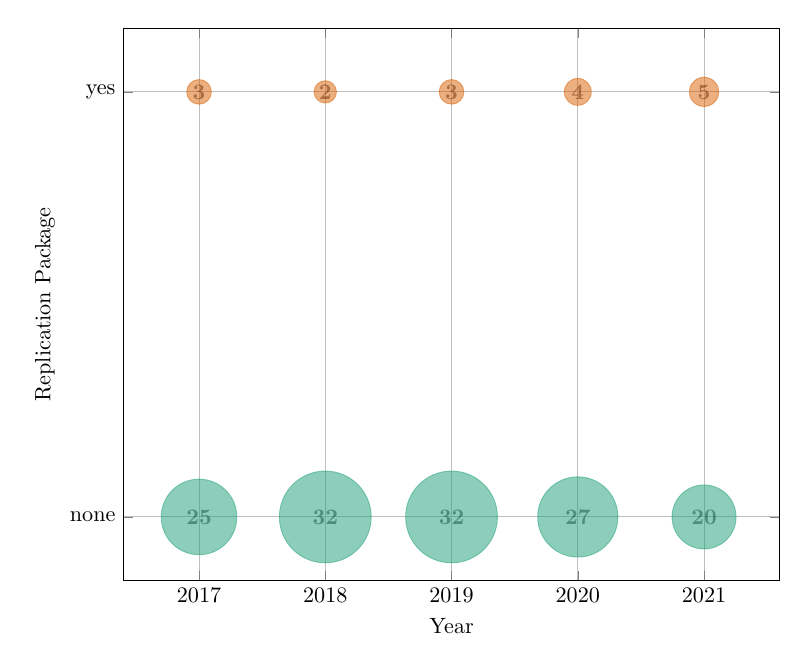
\begin{tikzpicture}[scale=.8]
\pgfplotsset{cycle list/Dark2}
\begin{axis}[width=.99\linewidth,
    enlargelimits=0.15,
    %x tick label style={rotate=45,anchor=east},
    xtick={0,1,2,3,4}, xticklabels={2017,2018,2019,2020,2021},
    xlabel={Year},
    ytick={0,1}, yticklabels={none,yes},
    ylabel={Replication Package},
    grid=both,
    scatter,scatter src=y,
    scatter/classes={0={draw=Dark2-A,fill=Dark2-A}, 1={draw=Dark2-B,fill=Dark2-B}}
]

\addplot+[mark=*,mark size=17.072,opacity=0.5,text=black] coordinates { (0,0) } node[text=black,font=\bfseries] {25};
\addplot+[mark=*,mark size=5.569,opacity=0.5,text=black] coordinates { (0,1) } node[text=black,font=\bfseries] {3};
\addplot+[mark=*,mark size=20.732,opacity=0.5,text=black] coordinates { (1,0) } node[text=black,font=\bfseries] {32};
\addplot+[mark=*,mark size=5.046,opacity=0.5,text=black] coordinates { (1,1) } node[text=black,font=\bfseries] {2};
\addplot+[mark=*,mark size=20.732,opacity=0.5,text=black] coordinates { (2,0) } node[text=black,font=\bfseries] {32};
\addplot+[mark=*,mark size=5.569,opacity=0.5,text=black] coordinates { (2,1) } node[text=black,font=\bfseries] {3};
\addplot+[mark=*,mark size=18.118,opacity=0.5,text=black] coordinates { (3,0) } node[text=black,font=\bfseries] {27};
\addplot+[mark=*,mark size=6.092,opacity=0.5,text=black] coordinates { (3,1) } node[text=black,font=\bfseries] {4};
\addplot+[mark=*,mark size=14.458,opacity=0.5,text=black] coordinates { (4,0) } node[text=black,font=\bfseries] {20};
\addplot+[mark=*,mark size=6.614,opacity=0.5,text=black] coordinates { (4,1) } node[text=black,font=\bfseries] {5};


\end{axis}
\end{tikzpicture}
\end{center}
%\caption{Portfolio f\"ur Year und Replication Package (Gr\"o\ss{}e entspricht der Anzahl)}\label{fig:port_year_replicationpackage}
%\end{figure}


%\subsection{Plot von Year je Replication Package}
%\begin{figure}
\begin{center}
\pgfplotsset{cycle list/Dark2}
\begin{tikzpicture}[scale=0.8]
\
\begin{axis}[ width=\linewidth, height=9cm,
    every axis plot/.append style={draw,mark=square},
    %nodes near coords,nodes near coords style={color=black,font=\small},
    enlargelimits=0.15, 
    bar width=3.5em,
    legend style={at={(0.5,1.1)}, anchor=north,legend columns=3},
    legend cell align={left},
    ylabel={Replication Package},ymajorgrids,ymin=0,
    %x tick label style={rotate=45,anchor=east},
    xtick={1,2,3,4,5}, xticklabels={2017,2018,2019,2020,2021},
    xlabel={Year},
    cycle multi list=Dark2
   ]
\addplot coordinates { (1,25)  (2,32)  (3,32)  (4,27)  (5,20)  };
\addplot coordinates { (1,3)  (2,2)  (3,3)  (4,4)  (5,5)  };

\legend{none,yes}
\end{axis}
\end{tikzpicture}
\end{center}
%\caption{Plot von Year je Replication Package}
%\label{fig:plot_year_replicationpackage}
%\end{figure}



%\subsection{Histogramm f\"ur Artifacts (153)}
%\begin{figure}
\begin{center}
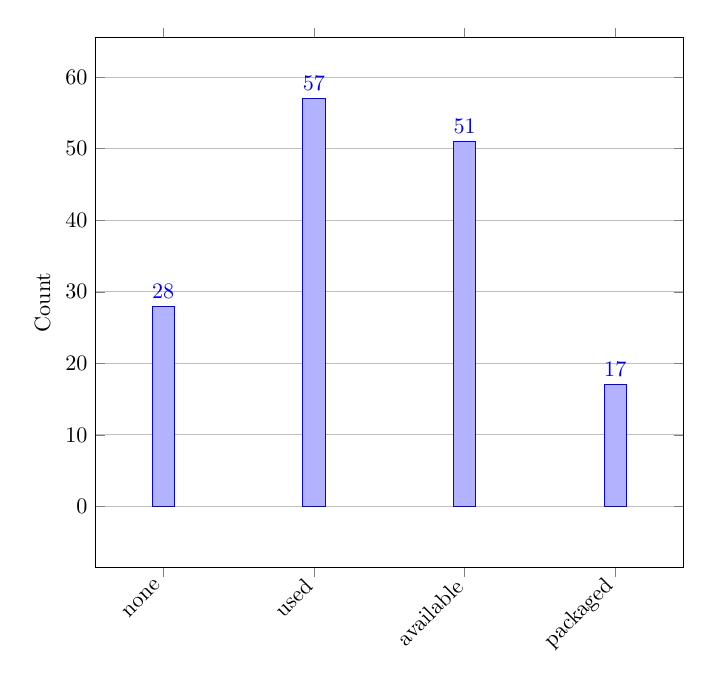
\begin{tikzpicture}[scale=.8]
\begin{axis}[ ybar, ymajorgrids, enlargelimits=0.15, legend style={at={(0.5,-0.15)}, anchor=north,legend columns=-1},
    width=.90\linewidth,height=10cm,
    nodes near coords, %nodes near coords align=below,
    ylabel={Count}, ymin=0,
    x tick label style={rotate=45,anchor=east},
    xtick={1,2,3,4},
    xticklabels={none,used,available,packaged
}
    %xlabel={Artifacts}    
    ]
  \addplot coordinates { (1,28)  (2,57)  (3,51)  (4,17)   };
\end{axis}
\end{tikzpicture}
\end{center}
%\caption{Histogramm f\"ur Artifacts (153)}
%\label{fig:histo_artifacts}
%\end{figure}


%\subsection{Pie chart for Artifacts (153)}
%\begin{figure}
\begin{center}
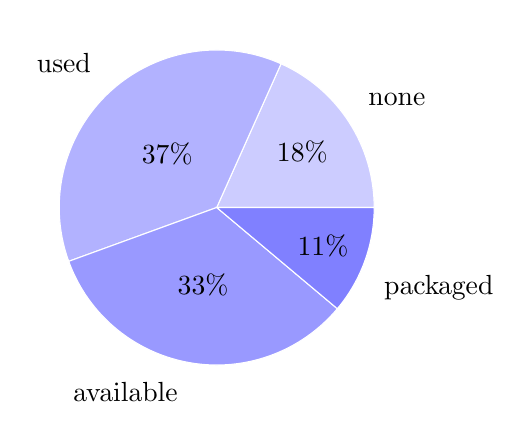
\begin{tikzpicture}[scale=2]
\pgfmathsetcounter{pief}{0}
\foreach \p/\q/\t/\c in {18/28/none/blue!20, 37/57/used/blue!30, 33/51/available/blue!40, 11/17/packaged/blue!50}
  {
    \setcounter{piee}{\value{pief}}
    \addtocounter{pief}{\q}
    \slice{\thepiee/153*360}
          {\thepief/153*360}
          {\p\%}{\t}{\c}
  }
\end{tikzpicture}

\textbf{Pie chart for Artifacts (153)}
\end{center}
%\caption{Pie chart for Artifacts (153)}
%\label{fig:pie_artifacts}
%\end{figure}


%\subsection{Histogram von Year je Artifacts}
%\begin{figure}
\begin{center}
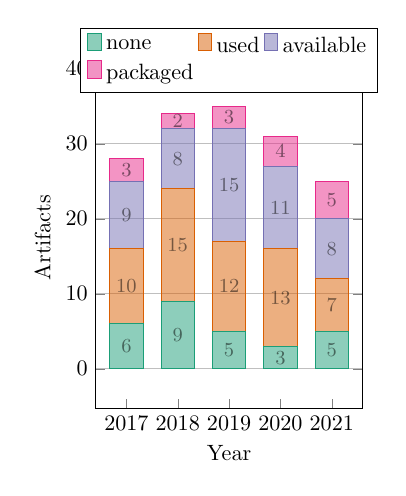
\begin{tikzpicture}[scale=0.8]
\pgfplotsset{cycle list/Dark2}
\begin{axis}[ width=.48\linewidth,height=7cm, ybar stacked,
    every axis plot/.append style={draw, fill, fill opacity=0.5},
    enlargelimits=0.15, 
    bar width=1.5em,
    nodes near coords, %nodes near coords align=below,
    nodes near coords style={color=black,font=\small},
    legend style={at={(0.5,1.115)}, anchor=north,legend columns=3},
    legend cell align={left},
    ylabel={Artifacts},ymajorgrids,ymin=0,
    %x tick label style={rotate=45,anchor=east},
    ymin=0,
    xtick={1,2,3,4,5}, xticklabels={2017,2018,2019,2020,2021},
    xlabel={Year},
    cycle multi list=Dark2    
   ]
\addplot coordinates { (1,6)  (2,9)  (3,5)  (4,3)  (5,5)  };
\addplot coordinates { (1,10)  (2,15)  (3,12)  (4,13)  (5,7)  };
\addplot coordinates { (1,9)  (2,8)  (3,15)  (4,11)  (5,8)  };
\addplot coordinates { (1,3)  (2,2)  (3,3)  (4,4)  (5,5)  };

\legend{none,used,available,packaged}
\end{axis}
\end{tikzpicture}
\end{center}
%\caption{Histogram von Year je Artifacts}
%\label{fig:chisto_year_artifacts}
%\end{figure}


%\subsection{Portfolio f\"ur Year und Artifacts (Gr\"o\ss{}e entspricht der Anzahl)}
%\begin{figure}
\begin{center}
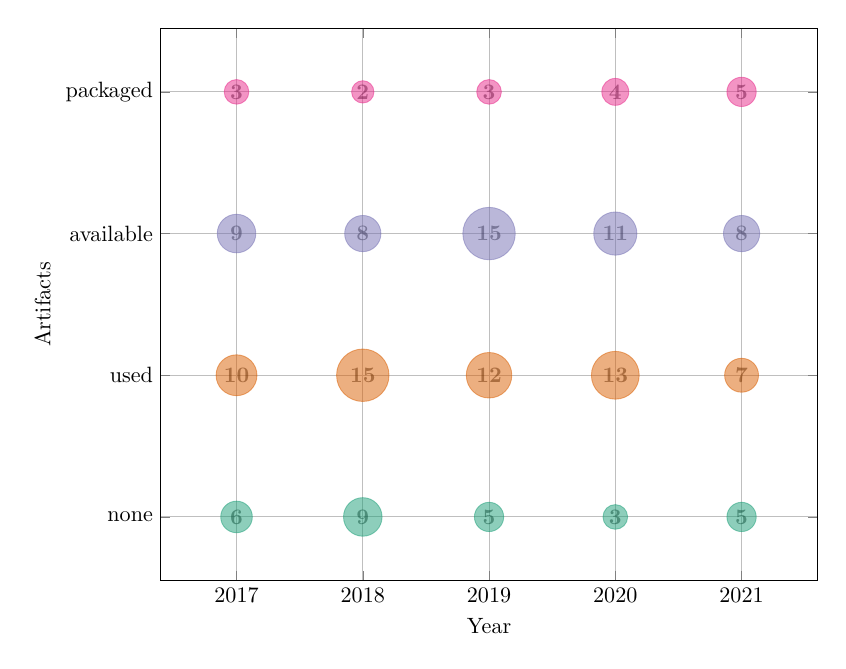
\begin{tikzpicture}[scale=.8]
\pgfplotsset{cycle list/Dark2}
\begin{axis}[width=.99\linewidth,
    enlargelimits=0.15,
    %x tick label style={rotate=45,anchor=east},
    xtick={0,1,2,3,4}, xticklabels={2017,2018,2019,2020,2021},
    xlabel={Year},
    ytick={0,1,2,3}, yticklabels={none,used,available,packaged},
    ylabel={Artifacts},
    grid=both,
    scatter,scatter src=y,
    scatter/classes={0={draw=Dark2-A,fill=Dark2-A}, 1={draw=Dark2-B,fill=Dark2-B}, 2={draw=Dark2-C,fill=Dark2-C}, 3={draw=Dark2-D,fill=Dark2-D}}
]

\addplot+[mark=*,mark size=7.137,opacity=0.5,text=black] coordinates { (0,0) } node[text=black,font=\bfseries] {6};
\addplot+[mark=*,mark size=9.229,opacity=0.5,text=black] coordinates { (0,1) } node[text=black,font=\bfseries] {10};
\addplot+[mark=*,mark size=8.706,opacity=0.5,text=black] coordinates { (0,2) } node[text=black,font=\bfseries] {9};
\addplot+[mark=*,mark size=5.569,opacity=0.5,text=black] coordinates { (0,3) } node[text=black,font=\bfseries] {3};
\addplot+[mark=*,mark size=8.706,opacity=0.5,text=black] coordinates { (1,0) } node[text=black,font=\bfseries] {9};
\addplot+[mark=*,mark size=11.843,opacity=0.5,text=black] coordinates { (1,1) } node[text=black,font=\bfseries] {15};
\addplot+[mark=*,mark size=8.183,opacity=0.5,text=black] coordinates { (1,2) } node[text=black,font=\bfseries] {8};
\addplot+[mark=*,mark size=5.046,opacity=0.5,text=black] coordinates { (1,3) } node[text=black,font=\bfseries] {2};
\addplot+[mark=*,mark size=6.614,opacity=0.5,text=black] coordinates { (2,0) } node[text=black,font=\bfseries] {5};
\addplot+[mark=*,mark size=10.275,opacity=0.5,text=black] coordinates { (2,1) } node[text=black,font=\bfseries] {12};
\addplot+[mark=*,mark size=11.843,opacity=0.5,text=black] coordinates { (2,2) } node[text=black,font=\bfseries] {15};
\addplot+[mark=*,mark size=5.569,opacity=0.5,text=black] coordinates { (2,3) } node[text=black,font=\bfseries] {3};
\addplot+[mark=*,mark size=5.569,opacity=0.5,text=black] coordinates { (3,0) } node[text=black,font=\bfseries] {3};
\addplot+[mark=*,mark size=10.797,opacity=0.5,text=black] coordinates { (3,1) } node[text=black,font=\bfseries] {13};
\addplot+[mark=*,mark size=9.752,opacity=0.5,text=black] coordinates { (3,2) } node[text=black,font=\bfseries] {11};
\addplot+[mark=*,mark size=6.092,opacity=0.5,text=black] coordinates { (3,3) } node[text=black,font=\bfseries] {4};
\addplot+[mark=*,mark size=6.614,opacity=0.5,text=black] coordinates { (4,0) } node[text=black,font=\bfseries] {5};
\addplot+[mark=*,mark size=7.660,opacity=0.5,text=black] coordinates { (4,1) } node[text=black,font=\bfseries] {7};
\addplot+[mark=*,mark size=8.183,opacity=0.5,text=black] coordinates { (4,2) } node[text=black,font=\bfseries] {8};
\addplot+[mark=*,mark size=6.614,opacity=0.5,text=black] coordinates { (4,3) } node[text=black,font=\bfseries] {5};


\end{axis}
\end{tikzpicture}
\end{center}
%\caption{Portfolio f\"ur Year und Artifacts (Gr\"o\ss{}e entspricht der Anzahl)}\label{fig:port_year_artifacts}
%\end{figure}


%\subsection{Plot von Year je Artifacts}
%\begin{figure}
\begin{center}
\pgfplotsset{cycle list/Dark2}
\begin{tikzpicture}[scale=0.8]
\
\begin{axis}[ width=\linewidth, height=9cm,
    every axis plot/.append style={draw,mark=square},
    %nodes near coords,nodes near coords style={color=black,font=\small},
    enlargelimits=0.15, 
    bar width=3.5em,
    legend style={at={(0.5,1.1)}, anchor=north,legend columns=3},
    legend cell align={left},
    ylabel={Artifacts},ymajorgrids,ymin=0,
    %x tick label style={rotate=45,anchor=east},
    xtick={1,2,3,4,5}, xticklabels={2017,2018,2019,2020,2021},
    xlabel={Year},
    cycle multi list=Dark2
   ]
\addplot coordinates { (1,6)  (2,9)  (3,5)  (4,3)  (5,5)  };
\addplot coordinates { (1,10)  (2,15)  (3,12)  (4,13)  (5,7)  };
\addplot coordinates { (1,9)  (2,8)  (3,15)  (4,11)  (5,8)  };
\addplot coordinates { (1,3)  (2,2)  (3,3)  (4,4)  (5,5)  };

\legend{none,used,available,packaged}
\end{axis}
\end{tikzpicture}
\end{center}
%\caption{Plot von Year je Artifacts}
%\label{fig:plot_year_artifacts}
%\end{figure}



\section{Threats to Validity}

%\subsection{Histogramm f\"ur Threats To Validity (293)}
%\begin{figure}
\begin{center}
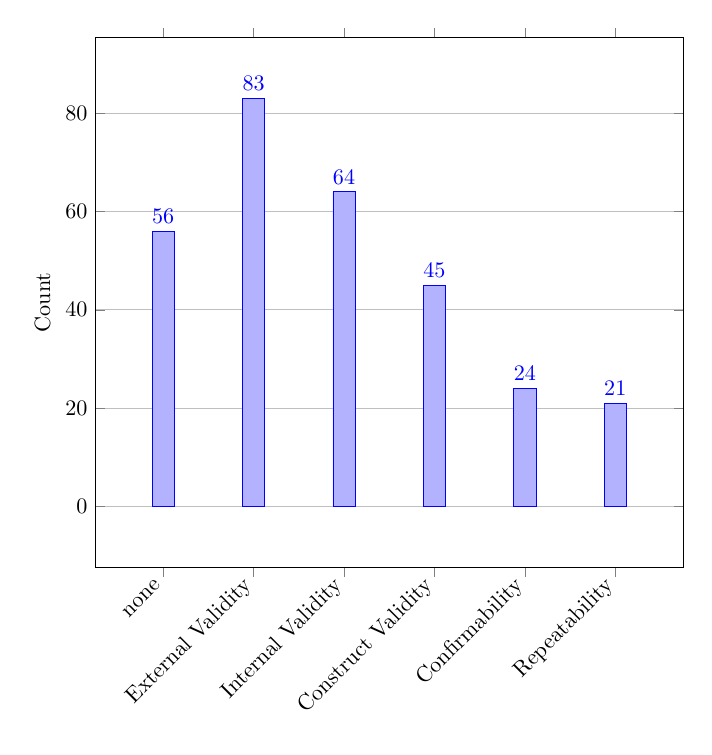
\begin{tikzpicture}[scale=.8]
\begin{axis}[ ybar, ymajorgrids, enlargelimits=0.15, legend style={at={(0.5,-0.15)}, anchor=north,legend columns=-1},
    width=.90\linewidth,height=10cm,
    nodes near coords, %nodes near coords align=below,
    ylabel={Count},ymin=0,
    x tick label style={rotate=45,anchor=east},
    xtick={1,2,3,4,5,6},
    xticklabels={none,External Validity,Internal Validity,Construct Validity,Confirmability,Repeatability
}
    %xlabel={Threats To Validity}    
    ]
  \addplot coordinates { (1,56)  (2,83)  (3,64)  (4,45)  (5,24)  (6,21)   };
\end{axis}
\end{tikzpicture}
\end{center}
%\caption{Histogramm f\"ur Threats To Validity (293)}
%\label{fig:histo_threatstovalidity}
%\end{figure}


%\subsection{Kreisdiagramm f\"ur Threats To Validity (293)}
%\begin{figure}
\begin{center}
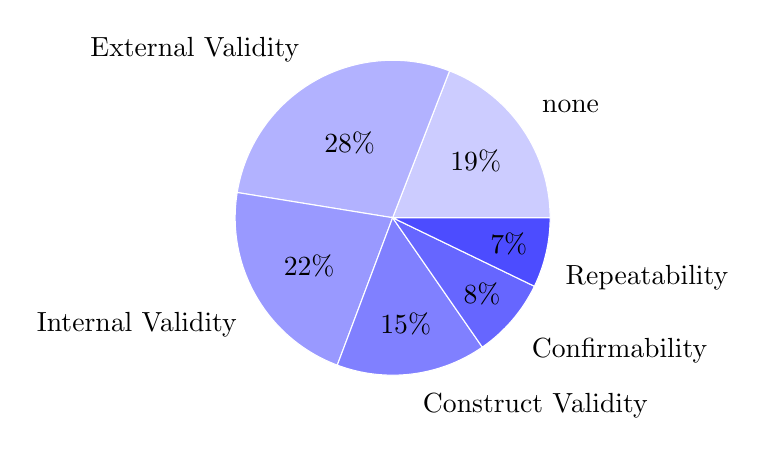
\begin{tikzpicture}[scale=2]
\pgfmathsetcounter{pieh}{0}
\foreach \p/\q/\t/\c in {19/56/none/blue!20, 28/83/External Validity/blue!30, 22/64/Internal Validity/blue!40, 15/45/Construct Validity/blue!50, 8/24/Confirmability/blue!60, 7/21/Repeatability/blue!70}
  {
    \setcounter{pieg}{\value{pieh}}
    \addtocounter{pieh}{\q}
    \slice{\thepieg/293*360}
          {\thepieh/293*360}
          {\p\%}{\t}{\c}
  }
\end{tikzpicture}
\end{center}
%\caption{Kreisdiagramm f\"ur Threats To Validity (293)}
%\label{fig:pie_threatstovalidity}
%\end{figure}


%\subsection{Histogram von Year je Threats To Validity}
%\begin{figure}
\begin{center}
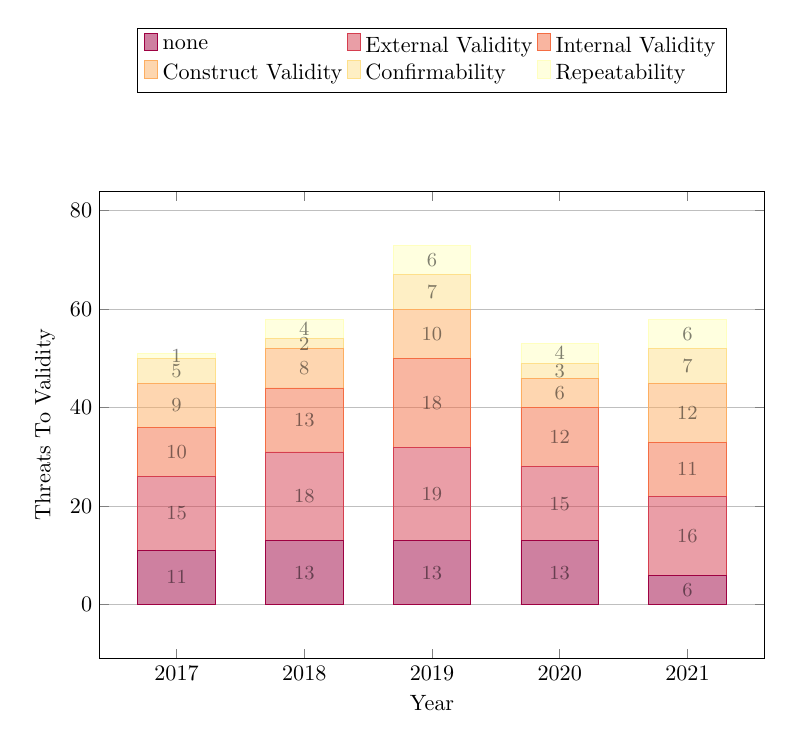
\begin{tikzpicture}[scale=0.8]
\
\begin{axis}[ width=\linewidth,height=9cm, ybar stacked,
    cycle multi list=Spectral,
    every axis plot/.append style={draw, fill, fill opacity=0.5},
    enlargelimits=0.15, 
    bar width=3.5em,
    nodes near coords, %nodes near coords align=below,
    nodes near coords style={color=black,font=\small},
    legend style={at={(0.5,1.35)}, anchor=north,legend columns=3},
    legend cell align={left},
    ylabel={Threats To Validity},ymajorgrids,ymin=0,
    %x tick label style={rotate=45,anchor=east},
    xtick={1,2,3,4,5}, xticklabels={2017,2018,2019,2020,2021},
    xlabel={Year}    
   ]
\addplot coordinates { (1,11)  (2,13)  (3,13)  (4,13)  (5,6)  };
\addplot coordinates { (1,15)  (2,18)  (3,19)  (4,15)  (5,16)  };
\addplot coordinates { (1,10)  (2,13)  (3,18)  (4,12)  (5,11)  };
\addplot coordinates { (1,9)  (2,8)  (3,10)  (4,6)  (5,12)  };
\addplot coordinates { (1,5)  (2,2)  (3,7)  (4,3)  (5,7)  };
\addplot coordinates { (1,1)  (2,4)  (3,6)  (4,4)  (5,6)  };

\legend{none,External Validity,Internal Validity,Construct Validity,Confirmability,Repeatability}
\end{axis}
\end{tikzpicture}
\end{center}
%\caption{Histogram von Year je Threats To Validity}
%\label{fig:chisto_year_threatstovalidity}
%\end{figure}



\section{Research Object vs. Evaluation Method}

%\subsection{Portfolio f\"ur Research Object und Evaluation Method (Gr\"o\ss{}e entspricht der Anzahl)}
%\begin{figure}
\begin{center}
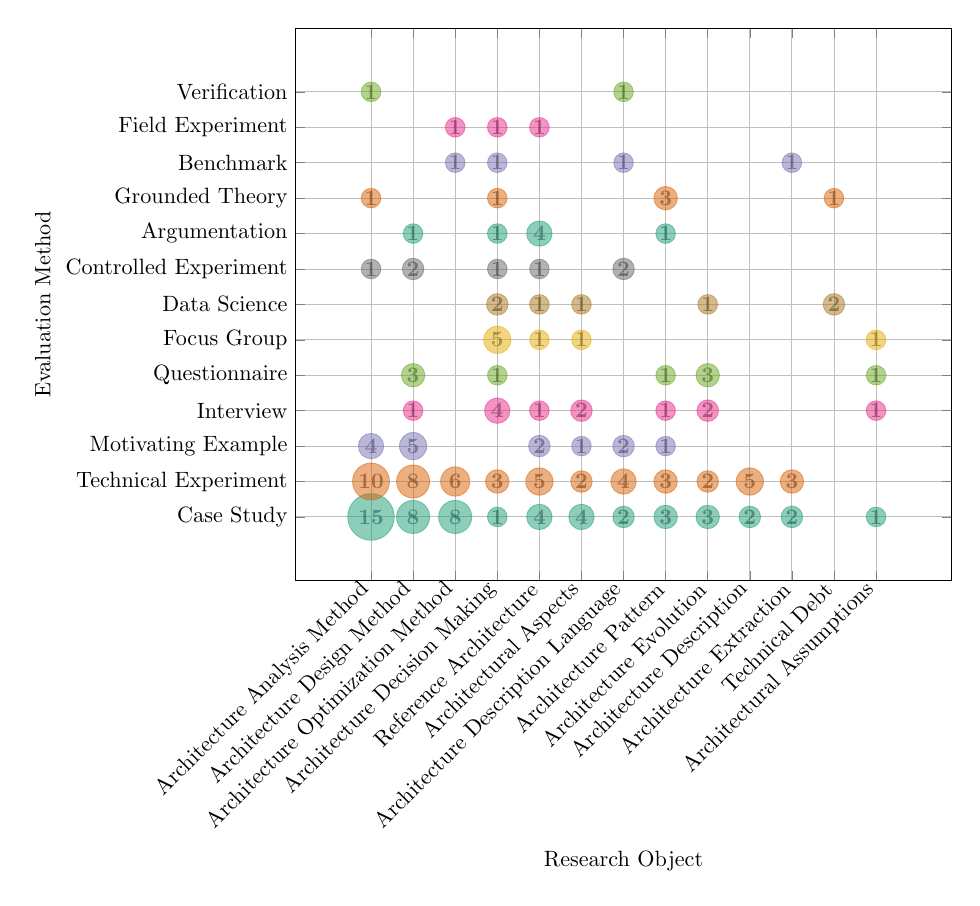
\begin{tikzpicture}[scale=.8]
\pgfplotsset{cycle list/Dark2}
\begin{axis}[width=.99\linewidth,
    enlargelimits=0.15,
    x tick label style={rotate=45,anchor=east},
    xtick={0,1,2,3,4,5,6,7,8,9,10,11,12}, xticklabels={Architecture Analysis Method,Architecture Design Method,Architecture Optimization Method,Architecture Decision Making,Reference Architecture,Architectural Aspects,Architecture Description Language,Architecture Pattern,Architecture Evolution,Architecture Description,Architecture Extraction,Technical Debt,Architectural Assumptions},
    xlabel={Research Object},
    ytick={0,1,2,3,4,5,6,7,8,9,10,11,12}, yticklabels={Case Study,Technical Experiment,Motivating Example,Interview,Questionnaire,Focus Group,Data Science,Controlled Experiment,Argumentation,Grounded Theory,Benchmark,Field Experiment,Verification},
    ylabel={Evaluation Method},
    grid=both,
    scatter,scatter src=y,
    scatter/classes={0={draw=Dark2-A,fill=Dark2-A}, 1={draw=Dark2-B,fill=Dark2-B}, 2={draw=Dark2-C,fill=Dark2-C}, 3={draw=Dark2-D,fill=Dark2-D}, 4={draw=Dark2-E,fill=Dark2-E}, 5={draw=Dark2-F,fill=Dark2-F}, 6={draw=Dark2-G,fill=Dark2-G}, 7={draw=Dark2-H,fill=Dark2-H}, 8={draw=Dark2-A,fill=Dark2-A}, 9={draw=Dark2-B,fill=Dark2-B}, 10={draw=Dark2-C,fill=Dark2-C}, 11={draw=Dark2-D,fill=Dark2-D}, 12={draw=Dark2-E,fill=Dark2-E}}
]

\addplot+[mark=*,mark size=10.522,opacity=0.5,text=black] coordinates { (0,0) } node[text=black,font=\bfseries] {15};
\addplot+[mark=*,mark size=8.348,opacity=0.5,text=black] coordinates { (0,1) } node[text=black,font=\bfseries] {10};
\addplot+[mark=*,mark size=5.739,opacity=0.5,text=black] coordinates { (0,2) } node[text=black,font=\bfseries] {4};
\addplot+[mark=*,mark size=4.435,opacity=0.5,text=black] coordinates { (0,7) } node[text=black,font=\bfseries] {1};
\addplot+[mark=*,mark size=4.435,opacity=0.5,text=black] coordinates { (0,9) } node[text=black,font=\bfseries] {1};
\addplot+[mark=*,mark size=4.435,opacity=0.5,text=black] coordinates { (0,12) } node[text=black,font=\bfseries] {1};
\addplot+[mark=*,mark size=7.478,opacity=0.5,text=black] coordinates { (1,0) } node[text=black,font=\bfseries] {8};
\addplot+[mark=*,mark size=7.478,opacity=0.5,text=black] coordinates { (1,1) } node[text=black,font=\bfseries] {8};
\addplot+[mark=*,mark size=6.174,opacity=0.5,text=black] coordinates { (1,2) } node[text=black,font=\bfseries] {5};
\addplot+[mark=*,mark size=4.435,opacity=0.5,text=black] coordinates { (1,3) } node[text=black,font=\bfseries] {1};
\addplot+[mark=*,mark size=5.304,opacity=0.5,text=black] coordinates { (1,4) } node[text=black,font=\bfseries] {3};
\addplot+[mark=*,mark size=4.870,opacity=0.5,text=black] coordinates { (1,7) } node[text=black,font=\bfseries] {2};
\addplot+[mark=*,mark size=4.435,opacity=0.5,text=black] coordinates { (1,8) } node[text=black,font=\bfseries] {1};
\addplot+[mark=*,mark size=7.478,opacity=0.5,text=black] coordinates { (2,0) } node[text=black,font=\bfseries] {8};
\addplot+[mark=*,mark size=6.609,opacity=0.5,text=black] coordinates { (2,1) } node[text=black,font=\bfseries] {6};
\addplot+[mark=*,mark size=4.435,opacity=0.5,text=black] coordinates { (2,10) } node[text=black,font=\bfseries] {1};
\addplot+[mark=*,mark size=4.435,opacity=0.5,text=black] coordinates { (2,11) } node[text=black,font=\bfseries] {1};
\addplot+[mark=*,mark size=4.435,opacity=0.5,text=black] coordinates { (3,0) } node[text=black,font=\bfseries] {1};
\addplot+[mark=*,mark size=5.304,opacity=0.5,text=black] coordinates { (3,1) } node[text=black,font=\bfseries] {3};
\addplot+[mark=*,mark size=5.739,opacity=0.5,text=black] coordinates { (3,3) } node[text=black,font=\bfseries] {4};
\addplot+[mark=*,mark size=4.435,opacity=0.5,text=black] coordinates { (3,4) } node[text=black,font=\bfseries] {1};
\addplot+[mark=*,mark size=6.174,opacity=0.5,text=black] coordinates { (3,5) } node[text=black,font=\bfseries] {5};
\addplot+[mark=*,mark size=4.870,opacity=0.5,text=black] coordinates { (3,6) } node[text=black,font=\bfseries] {2};
\addplot+[mark=*,mark size=4.435,opacity=0.5,text=black] coordinates { (3,7) } node[text=black,font=\bfseries] {1};
\addplot+[mark=*,mark size=4.435,opacity=0.5,text=black] coordinates { (3,8) } node[text=black,font=\bfseries] {1};
\addplot+[mark=*,mark size=4.435,opacity=0.5,text=black] coordinates { (3,9) } node[text=black,font=\bfseries] {1};
\addplot+[mark=*,mark size=4.435,opacity=0.5,text=black] coordinates { (3,10) } node[text=black,font=\bfseries] {1};
\addplot+[mark=*,mark size=4.435,opacity=0.5,text=black] coordinates { (3,11) } node[text=black,font=\bfseries] {1};
\addplot+[mark=*,mark size=5.739,opacity=0.5,text=black] coordinates { (4,0) } node[text=black,font=\bfseries] {4};
\addplot+[mark=*,mark size=6.174,opacity=0.5,text=black] coordinates { (4,1) } node[text=black,font=\bfseries] {5};
\addplot+[mark=*,mark size=4.870,opacity=0.5,text=black] coordinates { (4,2) } node[text=black,font=\bfseries] {2};
\addplot+[mark=*,mark size=4.435,opacity=0.5,text=black] coordinates { (4,3) } node[text=black,font=\bfseries] {1};
\addplot+[mark=*,mark size=4.435,opacity=0.5,text=black] coordinates { (4,5) } node[text=black,font=\bfseries] {1};
\addplot+[mark=*,mark size=4.435,opacity=0.5,text=black] coordinates { (4,6) } node[text=black,font=\bfseries] {1};
\addplot+[mark=*,mark size=4.435,opacity=0.5,text=black] coordinates { (4,7) } node[text=black,font=\bfseries] {1};
\addplot+[mark=*,mark size=5.739,opacity=0.5,text=black] coordinates { (4,8) } node[text=black,font=\bfseries] {4};
\addplot+[mark=*,mark size=4.435,opacity=0.5,text=black] coordinates { (4,11) } node[text=black,font=\bfseries] {1};
\addplot+[mark=*,mark size=5.739,opacity=0.5,text=black] coordinates { (5,0) } node[text=black,font=\bfseries] {4};
\addplot+[mark=*,mark size=4.870,opacity=0.5,text=black] coordinates { (5,1) } node[text=black,font=\bfseries] {2};
\addplot+[mark=*,mark size=4.435,opacity=0.5,text=black] coordinates { (5,2) } node[text=black,font=\bfseries] {1};
\addplot+[mark=*,mark size=4.870,opacity=0.5,text=black] coordinates { (5,3) } node[text=black,font=\bfseries] {2};
\addplot+[mark=*,mark size=4.435,opacity=0.5,text=black] coordinates { (5,5) } node[text=black,font=\bfseries] {1};
\addplot+[mark=*,mark size=4.435,opacity=0.5,text=black] coordinates { (5,6) } node[text=black,font=\bfseries] {1};
\addplot+[mark=*,mark size=4.870,opacity=0.5,text=black] coordinates { (6,0) } node[text=black,font=\bfseries] {2};
\addplot+[mark=*,mark size=5.739,opacity=0.5,text=black] coordinates { (6,1) } node[text=black,font=\bfseries] {4};
\addplot+[mark=*,mark size=4.870,opacity=0.5,text=black] coordinates { (6,2) } node[text=black,font=\bfseries] {2};
\addplot+[mark=*,mark size=4.870,opacity=0.5,text=black] coordinates { (6,7) } node[text=black,font=\bfseries] {2};
\addplot+[mark=*,mark size=4.435,opacity=0.5,text=black] coordinates { (6,10) } node[text=black,font=\bfseries] {1};
\addplot+[mark=*,mark size=4.435,opacity=0.5,text=black] coordinates { (6,12) } node[text=black,font=\bfseries] {1};
\addplot+[mark=*,mark size=5.304,opacity=0.5,text=black] coordinates { (7,0) } node[text=black,font=\bfseries] {3};
\addplot+[mark=*,mark size=5.304,opacity=0.5,text=black] coordinates { (7,1) } node[text=black,font=\bfseries] {3};
\addplot+[mark=*,mark size=4.435,opacity=0.5,text=black] coordinates { (7,2) } node[text=black,font=\bfseries] {1};
\addplot+[mark=*,mark size=4.435,opacity=0.5,text=black] coordinates { (7,3) } node[text=black,font=\bfseries] {1};
\addplot+[mark=*,mark size=4.435,opacity=0.5,text=black] coordinates { (7,4) } node[text=black,font=\bfseries] {1};
\addplot+[mark=*,mark size=4.435,opacity=0.5,text=black] coordinates { (7,8) } node[text=black,font=\bfseries] {1};
\addplot+[mark=*,mark size=5.304,opacity=0.5,text=black] coordinates { (7,9) } node[text=black,font=\bfseries] {3};
\addplot+[mark=*,mark size=5.304,opacity=0.5,text=black] coordinates { (8,0) } node[text=black,font=\bfseries] {3};
\addplot+[mark=*,mark size=4.870,opacity=0.5,text=black] coordinates { (8,1) } node[text=black,font=\bfseries] {2};
\addplot+[mark=*,mark size=4.870,opacity=0.5,text=black] coordinates { (8,3) } node[text=black,font=\bfseries] {2};
\addplot+[mark=*,mark size=5.304,opacity=0.5,text=black] coordinates { (8,4) } node[text=black,font=\bfseries] {3};
\addplot+[mark=*,mark size=4.435,opacity=0.5,text=black] coordinates { (8,6) } node[text=black,font=\bfseries] {1};
\addplot+[mark=*,mark size=4.870,opacity=0.5,text=black] coordinates { (9,0) } node[text=black,font=\bfseries] {2};
\addplot+[mark=*,mark size=6.174,opacity=0.5,text=black] coordinates { (9,1) } node[text=black,font=\bfseries] {5};
\addplot+[mark=*,mark size=4.870,opacity=0.5,text=black] coordinates { (10,0) } node[text=black,font=\bfseries] {2};
\addplot+[mark=*,mark size=5.304,opacity=0.5,text=black] coordinates { (10,1) } node[text=black,font=\bfseries] {3};
\addplot+[mark=*,mark size=4.435,opacity=0.5,text=black] coordinates { (10,10) } node[text=black,font=\bfseries] {1};
\addplot+[mark=*,mark size=4.870,opacity=0.5,text=black] coordinates { (11,6) } node[text=black,font=\bfseries] {2};
\addplot+[mark=*,mark size=4.435,opacity=0.5,text=black] coordinates { (11,9) } node[text=black,font=\bfseries] {1};
\addplot+[mark=*,mark size=4.435,opacity=0.5,text=black] coordinates { (12,0) } node[text=black,font=\bfseries] {1};
\addplot+[mark=*,mark size=4.435,opacity=0.5,text=black] coordinates { (12,3) } node[text=black,font=\bfseries] {1};
\addplot+[mark=*,mark size=4.435,opacity=0.5,text=black] coordinates { (12,4) } node[text=black,font=\bfseries] {1};
\addplot+[mark=*,mark size=4.435,opacity=0.5,text=black] coordinates { (12,5) } node[text=black,font=\bfseries] {1};


\end{axis}
\end{tikzpicture}
\end{center}
%\caption{Portfolio f\"ur Research Object und Evaluation Method (Gr\"o\ss{}e entspricht der Anzahl)}\label{fig:port_researchobject_evaluationmethod}
%\end{figure}


%\subsection{Portfolio f\"ur Evaluation Method und Research Object (Gr\"o\ss{}e entspricht der Anzahl)}
%\begin{figure}
\begin{center}
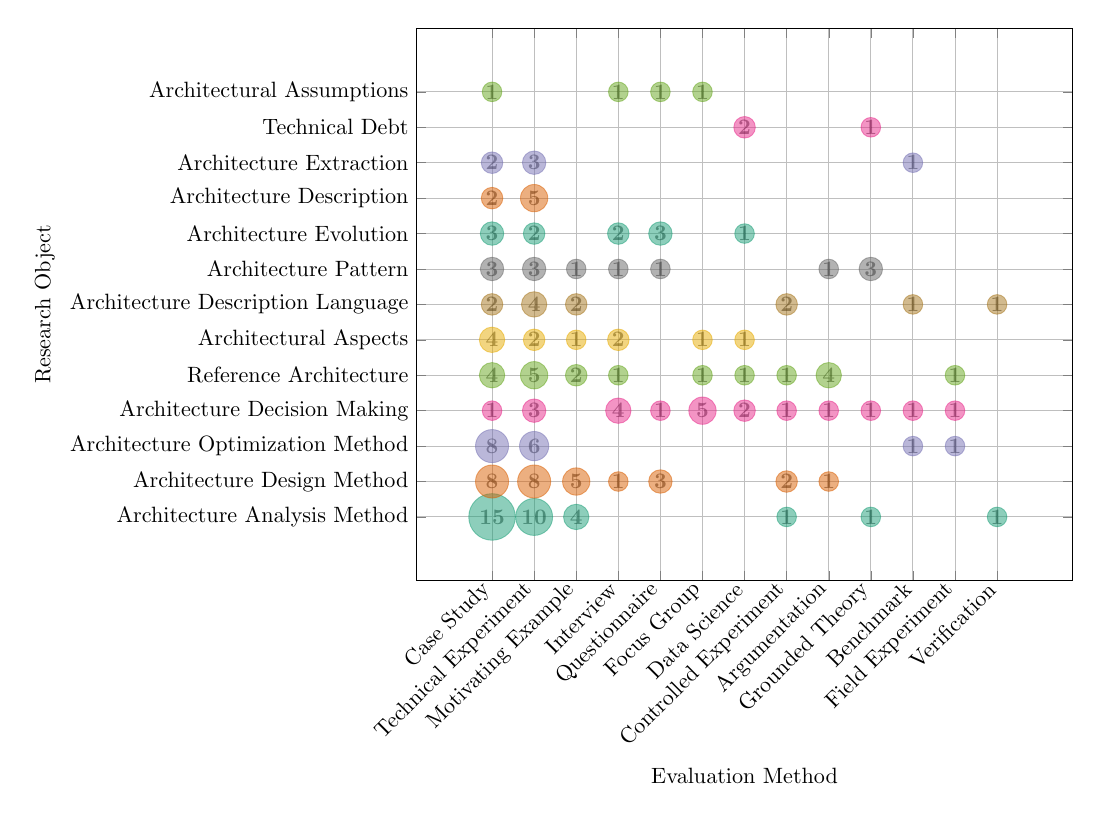
\begin{tikzpicture}[scale=.8]
\pgfplotsset{cycle list/Dark2}
\begin{axis}[width=.99\linewidth,
    enlargelimits=0.15,
    x tick label style={rotate=45,anchor=east},
    xtick={0,1,2,3,4,5,6,7,8,9,10,11,12}, xticklabels={Case Study,Technical Experiment,Motivating Example,Interview,Questionnaire,Focus Group,Data Science,Controlled Experiment,Argumentation,Grounded Theory,Benchmark,Field Experiment,Verification},
    xlabel={Evaluation Method},
    ytick={0,1,2,3,4,5,6,7,8,9,10,11,12}, yticklabels={Architecture Analysis Method,Architecture Design Method,Architecture Optimization Method,Architecture Decision Making,Reference Architecture,Architectural Aspects,Architecture Description Language,Architecture Pattern,Architecture Evolution,Architecture Description,Architecture Extraction,Technical Debt,Architectural Assumptions},
    ylabel={Research Object},
    grid=both,
    scatter,scatter src=y,
    scatter/classes={0={draw=Dark2-A,fill=Dark2-A}, 1={draw=Dark2-B,fill=Dark2-B}, 2={draw=Dark2-C,fill=Dark2-C}, 3={draw=Dark2-D,fill=Dark2-D}, 4={draw=Dark2-E,fill=Dark2-E}, 5={draw=Dark2-F,fill=Dark2-F}, 6={draw=Dark2-G,fill=Dark2-G}, 7={draw=Dark2-H,fill=Dark2-H}, 8={draw=Dark2-A,fill=Dark2-A}, 9={draw=Dark2-B,fill=Dark2-B}, 10={draw=Dark2-C,fill=Dark2-C}, 11={draw=Dark2-D,fill=Dark2-D}, 12={draw=Dark2-E,fill=Dark2-E}}
]

\addplot+[mark=*,mark size=10.522,opacity=0.5,text=black] coordinates { (0,0) } node[text=black,font=\bfseries] {15};
\addplot+[mark=*,mark size=7.478,opacity=0.5,text=black] coordinates { (0,1) } node[text=black,font=\bfseries] {8};
\addplot+[mark=*,mark size=7.478,opacity=0.5,text=black] coordinates { (0,2) } node[text=black,font=\bfseries] {8};
\addplot+[mark=*,mark size=4.435,opacity=0.5,text=black] coordinates { (0,3) } node[text=black,font=\bfseries] {1};
\addplot+[mark=*,mark size=5.739,opacity=0.5,text=black] coordinates { (0,4) } node[text=black,font=\bfseries] {4};
\addplot+[mark=*,mark size=5.739,opacity=0.5,text=black] coordinates { (0,5) } node[text=black,font=\bfseries] {4};
\addplot+[mark=*,mark size=4.870,opacity=0.5,text=black] coordinates { (0,6) } node[text=black,font=\bfseries] {2};
\addplot+[mark=*,mark size=5.304,opacity=0.5,text=black] coordinates { (0,7) } node[text=black,font=\bfseries] {3};
\addplot+[mark=*,mark size=5.304,opacity=0.5,text=black] coordinates { (0,8) } node[text=black,font=\bfseries] {3};
\addplot+[mark=*,mark size=4.870,opacity=0.5,text=black] coordinates { (0,9) } node[text=black,font=\bfseries] {2};
\addplot+[mark=*,mark size=4.870,opacity=0.5,text=black] coordinates { (0,10) } node[text=black,font=\bfseries] {2};
\addplot+[mark=*,mark size=4.435,opacity=0.5,text=black] coordinates { (0,12) } node[text=black,font=\bfseries] {1};
\addplot+[mark=*,mark size=8.348,opacity=0.5,text=black] coordinates { (1,0) } node[text=black,font=\bfseries] {10};
\addplot+[mark=*,mark size=7.478,opacity=0.5,text=black] coordinates { (1,1) } node[text=black,font=\bfseries] {8};
\addplot+[mark=*,mark size=6.609,opacity=0.5,text=black] coordinates { (1,2) } node[text=black,font=\bfseries] {6};
\addplot+[mark=*,mark size=5.304,opacity=0.5,text=black] coordinates { (1,3) } node[text=black,font=\bfseries] {3};
\addplot+[mark=*,mark size=6.174,opacity=0.5,text=black] coordinates { (1,4) } node[text=black,font=\bfseries] {5};
\addplot+[mark=*,mark size=4.870,opacity=0.5,text=black] coordinates { (1,5) } node[text=black,font=\bfseries] {2};
\addplot+[mark=*,mark size=5.739,opacity=0.5,text=black] coordinates { (1,6) } node[text=black,font=\bfseries] {4};
\addplot+[mark=*,mark size=5.304,opacity=0.5,text=black] coordinates { (1,7) } node[text=black,font=\bfseries] {3};
\addplot+[mark=*,mark size=4.870,opacity=0.5,text=black] coordinates { (1,8) } node[text=black,font=\bfseries] {2};
\addplot+[mark=*,mark size=6.174,opacity=0.5,text=black] coordinates { (1,9) } node[text=black,font=\bfseries] {5};
\addplot+[mark=*,mark size=5.304,opacity=0.5,text=black] coordinates { (1,10) } node[text=black,font=\bfseries] {3};
\addplot+[mark=*,mark size=5.739,opacity=0.5,text=black] coordinates { (2,0) } node[text=black,font=\bfseries] {4};
\addplot+[mark=*,mark size=6.174,opacity=0.5,text=black] coordinates { (2,1) } node[text=black,font=\bfseries] {5};
\addplot+[mark=*,mark size=4.870,opacity=0.5,text=black] coordinates { (2,4) } node[text=black,font=\bfseries] {2};
\addplot+[mark=*,mark size=4.435,opacity=0.5,text=black] coordinates { (2,5) } node[text=black,font=\bfseries] {1};
\addplot+[mark=*,mark size=4.870,opacity=0.5,text=black] coordinates { (2,6) } node[text=black,font=\bfseries] {2};
\addplot+[mark=*,mark size=4.435,opacity=0.5,text=black] coordinates { (2,7) } node[text=black,font=\bfseries] {1};
\addplot+[mark=*,mark size=4.435,opacity=0.5,text=black] coordinates { (3,1) } node[text=black,font=\bfseries] {1};
\addplot+[mark=*,mark size=5.739,opacity=0.5,text=black] coordinates { (3,3) } node[text=black,font=\bfseries] {4};
\addplot+[mark=*,mark size=4.435,opacity=0.5,text=black] coordinates { (3,4) } node[text=black,font=\bfseries] {1};
\addplot+[mark=*,mark size=4.870,opacity=0.5,text=black] coordinates { (3,5) } node[text=black,font=\bfseries] {2};
\addplot+[mark=*,mark size=4.435,opacity=0.5,text=black] coordinates { (3,7) } node[text=black,font=\bfseries] {1};
\addplot+[mark=*,mark size=4.870,opacity=0.5,text=black] coordinates { (3,8) } node[text=black,font=\bfseries] {2};
\addplot+[mark=*,mark size=4.435,opacity=0.5,text=black] coordinates { (3,12) } node[text=black,font=\bfseries] {1};
\addplot+[mark=*,mark size=5.304,opacity=0.5,text=black] coordinates { (4,1) } node[text=black,font=\bfseries] {3};
\addplot+[mark=*,mark size=4.435,opacity=0.5,text=black] coordinates { (4,3) } node[text=black,font=\bfseries] {1};
\addplot+[mark=*,mark size=4.435,opacity=0.5,text=black] coordinates { (4,7) } node[text=black,font=\bfseries] {1};
\addplot+[mark=*,mark size=5.304,opacity=0.5,text=black] coordinates { (4,8) } node[text=black,font=\bfseries] {3};
\addplot+[mark=*,mark size=4.435,opacity=0.5,text=black] coordinates { (4,12) } node[text=black,font=\bfseries] {1};
\addplot+[mark=*,mark size=6.174,opacity=0.5,text=black] coordinates { (5,3) } node[text=black,font=\bfseries] {5};
\addplot+[mark=*,mark size=4.435,opacity=0.5,text=black] coordinates { (5,4) } node[text=black,font=\bfseries] {1};
\addplot+[mark=*,mark size=4.435,opacity=0.5,text=black] coordinates { (5,5) } node[text=black,font=\bfseries] {1};
\addplot+[mark=*,mark size=4.435,opacity=0.5,text=black] coordinates { (5,12) } node[text=black,font=\bfseries] {1};
\addplot+[mark=*,mark size=4.870,opacity=0.5,text=black] coordinates { (6,3) } node[text=black,font=\bfseries] {2};
\addplot+[mark=*,mark size=4.435,opacity=0.5,text=black] coordinates { (6,4) } node[text=black,font=\bfseries] {1};
\addplot+[mark=*,mark size=4.435,opacity=0.5,text=black] coordinates { (6,5) } node[text=black,font=\bfseries] {1};
\addplot+[mark=*,mark size=4.435,opacity=0.5,text=black] coordinates { (6,8) } node[text=black,font=\bfseries] {1};
\addplot+[mark=*,mark size=4.870,opacity=0.5,text=black] coordinates { (6,11) } node[text=black,font=\bfseries] {2};
\addplot+[mark=*,mark size=4.435,opacity=0.5,text=black] coordinates { (7,0) } node[text=black,font=\bfseries] {1};
\addplot+[mark=*,mark size=4.870,opacity=0.5,text=black] coordinates { (7,1) } node[text=black,font=\bfseries] {2};
\addplot+[mark=*,mark size=4.435,opacity=0.5,text=black] coordinates { (7,3) } node[text=black,font=\bfseries] {1};
\addplot+[mark=*,mark size=4.435,opacity=0.5,text=black] coordinates { (7,4) } node[text=black,font=\bfseries] {1};
\addplot+[mark=*,mark size=4.870,opacity=0.5,text=black] coordinates { (7,6) } node[text=black,font=\bfseries] {2};
\addplot+[mark=*,mark size=4.435,opacity=0.5,text=black] coordinates { (8,1) } node[text=black,font=\bfseries] {1};
\addplot+[mark=*,mark size=4.435,opacity=0.5,text=black] coordinates { (8,3) } node[text=black,font=\bfseries] {1};
\addplot+[mark=*,mark size=5.739,opacity=0.5,text=black] coordinates { (8,4) } node[text=black,font=\bfseries] {4};
\addplot+[mark=*,mark size=4.435,opacity=0.5,text=black] coordinates { (8,7) } node[text=black,font=\bfseries] {1};
\addplot+[mark=*,mark size=4.435,opacity=0.5,text=black] coordinates { (9,0) } node[text=black,font=\bfseries] {1};
\addplot+[mark=*,mark size=4.435,opacity=0.5,text=black] coordinates { (9,3) } node[text=black,font=\bfseries] {1};
\addplot+[mark=*,mark size=5.304,opacity=0.5,text=black] coordinates { (9,7) } node[text=black,font=\bfseries] {3};
\addplot+[mark=*,mark size=4.435,opacity=0.5,text=black] coordinates { (9,11) } node[text=black,font=\bfseries] {1};
\addplot+[mark=*,mark size=4.435,opacity=0.5,text=black] coordinates { (10,2) } node[text=black,font=\bfseries] {1};
\addplot+[mark=*,mark size=4.435,opacity=0.5,text=black] coordinates { (10,3) } node[text=black,font=\bfseries] {1};
\addplot+[mark=*,mark size=4.435,opacity=0.5,text=black] coordinates { (10,6) } node[text=black,font=\bfseries] {1};
\addplot+[mark=*,mark size=4.435,opacity=0.5,text=black] coordinates { (10,10) } node[text=black,font=\bfseries] {1};
\addplot+[mark=*,mark size=4.435,opacity=0.5,text=black] coordinates { (11,2) } node[text=black,font=\bfseries] {1};
\addplot+[mark=*,mark size=4.435,opacity=0.5,text=black] coordinates { (11,3) } node[text=black,font=\bfseries] {1};
\addplot+[mark=*,mark size=4.435,opacity=0.5,text=black] coordinates { (11,4) } node[text=black,font=\bfseries] {1};
\addplot+[mark=*,mark size=4.435,opacity=0.5,text=black] coordinates { (12,0) } node[text=black,font=\bfseries] {1};
\addplot+[mark=*,mark size=4.435,opacity=0.5,text=black] coordinates { (12,6) } node[text=black,font=\bfseries] {1};


\end{axis}
\end{tikzpicture}
\end{center}
%\caption{Portfolio f\"ur Evaluation Method und Research Object (Gr\"o\ss{}e entspricht der Anzahl)}\label{fig:port_evaluationmethod_researchobject}
%\end{figure}



\section{Research Object vs. Property}

%\subsection{Histogramm f\"ur Research Object (171)}
%\begin{figure}
\begin{center}
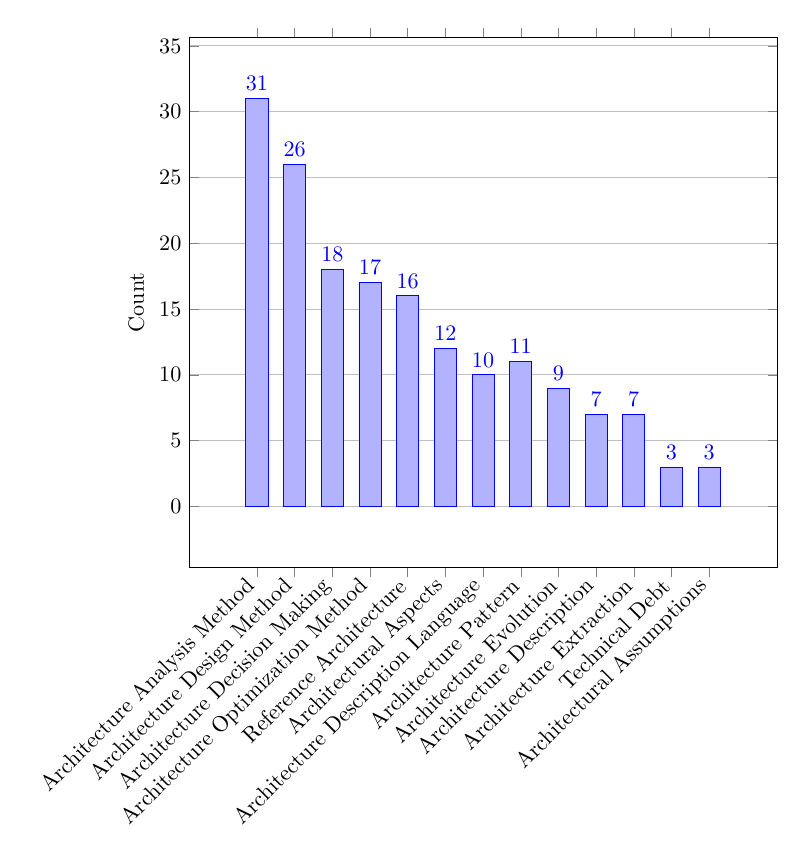
\begin{tikzpicture}[scale=.8]
\begin{axis}[ ybar, ymajorgrids, enlargelimits=0.15, legend style={at={(0.5,-0.15)}, anchor=north,legend columns=-1},
    width=.90\linewidth,height=10cm,
    nodes near coords, %nodes near coords align=below,
    ylabel={Count}, ymin=0,
    x tick label style={rotate=45,anchor=east},
    xtick={1,2,3,4,5,6,7,8,9,10,11,12,13},
    xticklabels={Architecture Analysis Method,Architecture Design Method,Architecture Decision Making,Architecture Optimization Method,Reference Architecture,Architectural Aspects,Architecture Description Language,Architecture Pattern,Architecture Evolution,Architecture Description,Architecture Extraction,Technical Debt,Architectural Assumptions
}
    %xlabel={Research Object}    
    ]
  \addplot coordinates { (1,31)  (2,26)  (3,18)  (4,17)  (5,16)  (6,12)  (7,10)  (8,11)  (9,9)  (10,7)  (11,7)  (12,3)  (13,3)   };
\end{axis}
\end{tikzpicture}
\end{center}
%\caption{Histogramm f\"ur Research Object (171)}
%\label{fig:histo_researchobject}
%\end{figure}


%\subsection{Histogramm f\"ur Property (299)}
%\begin{figure}
\begin{center}
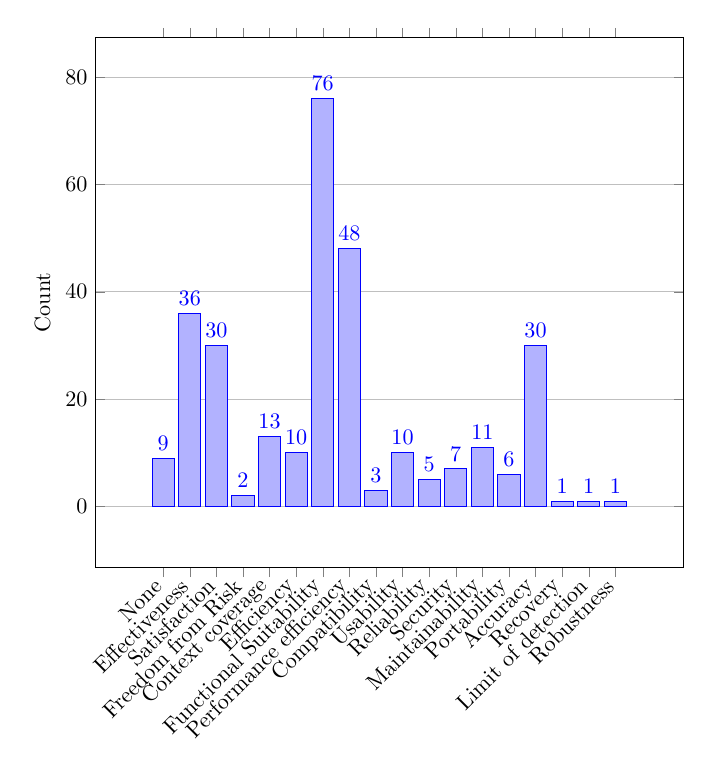
\begin{tikzpicture}[scale=.8]
\begin{axis}[ ybar, ymajorgrids, enlargelimits=0.15, legend style={at={(0.5,-0.15)}, anchor=north,legend columns=-1},
    width=.90\linewidth,height=10cm,
    nodes near coords, %nodes near coords align=below,
    ylabel={Count}, ymin=0,
    x tick label style={rotate=45,anchor=east},
    xtick={1,2,3,4,5,6,7,8,9,10,11,12,13,14,15,16,17,18},
    xticklabels={None,Effectiveness,Satisfaction,Freedom from Risk,Context coverage,Efficiency,Functional Suitability,Performance efficiency,Compatibility,Usability,Reliability,Security,Maintainability,Portability,Accuracy,Recovery,Limit of detection,Robustness
}
    %xlabel={Property}    
    ]
  \addplot coordinates { (1,9)  (2,36)  (3,30)  (4,2)  (5,13)  (6,10)  (7,76)  (8,48)  (9,3)  (10,10)  (11,5)  (12,7)  (13,11)  (14,6)  (15,30)  (16,1)  (17,1)  (18,1)   };
\end{axis}
\end{tikzpicture}
\end{center}
%\caption{Histogramm f\"ur Property (299)}
%\label{fig:histo_property}
%\end{figure}


%\subsection{Histogram von Year je Property}
%\begin{figure}
\begin{center}
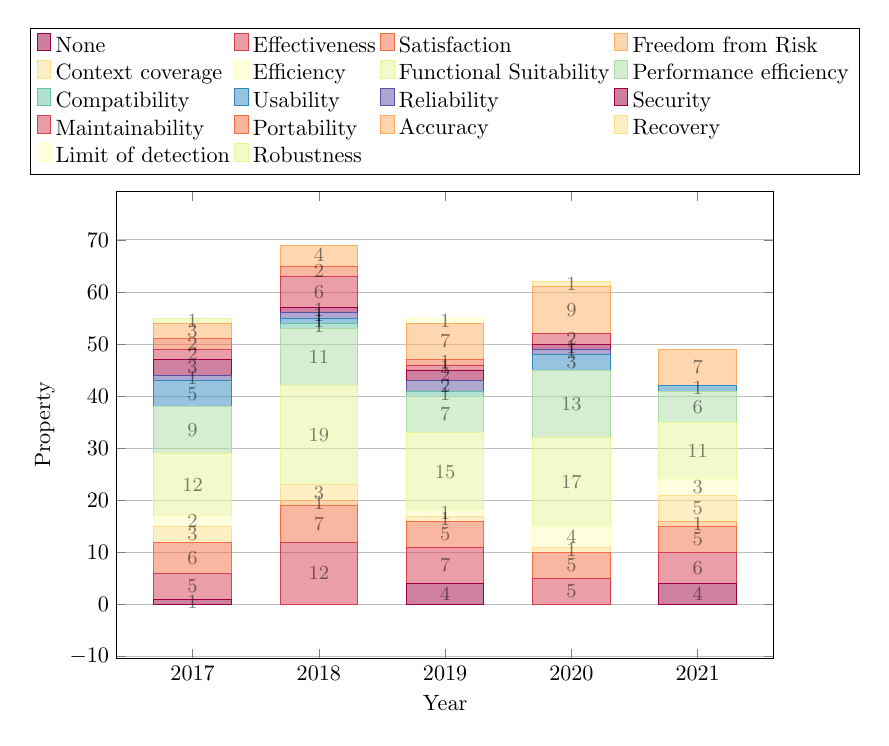
\begin{tikzpicture}[scale=0.8]
\
\begin{axis}[ width=.99\linewidth,height=9cm, ybar stacked,
    cycle multi list=Spectral,
    every axis plot/.append style={draw, fill, fill opacity=0.5},
    enlargelimits=0.15, 
    bar width=3.5em,
    nodes near coords, %nodes near coords align=below,
    nodes near coords style={color=black,font=\small},
    legend style={at={(0.5,1.35)}, anchor=north,legend columns=4},
    legend cell align={left},
    ylabel={Property},ymajorgrids, ymin=0, 
    %x tick label style={rotate=45,anchor=east},
    xtick={1,2,3,4,5}, xticklabels={2017,2018,2019,2020,2021},
    xlabel={Year}    
   ]
\addplot coordinates { (1,1)  (2,0)  (3,4)  (4,0)  (5,4)  };
\addplot coordinates { (1,5)  (2,12)  (3,7)  (4,5)  (5,6)  };
\addplot coordinates { (1,6)  (2,7)  (3,5)  (4,5)  (5,5)  };
\addplot coordinates { (1,0)  (2,1)  (3,0)  (4,0)  (5,1)  };
\addplot coordinates { (1,3)  (2,3)  (3,1)  (4,1)  (5,5)  };
\addplot coordinates { (1,2)  (2,0)  (3,1)  (4,4)  (5,3)  };
\addplot coordinates { (1,12)  (2,19)  (3,15)  (4,17)  (5,11)  };
\addplot coordinates { (1,9)  (2,11)  (3,7)  (4,13)  (5,6)  };
\addplot coordinates { (1,0)  (2,1)  (3,1)  (4,0)  (5,0)  };
\addplot coordinates { (1,5)  (2,1)  (3,0)  (4,3)  (5,1)  };
\addplot coordinates { (1,1)  (2,1)  (3,2)  (4,1)  (5,0)  };
\addplot coordinates { (1,3)  (2,1)  (3,2)  (4,1)  (5,0)  };
\addplot coordinates { (1,2)  (2,6)  (3,1)  (4,2)  (5,0)  };
\addplot coordinates { (1,2)  (2,2)  (3,1)  (4,0)  (5,0)  };
\addplot coordinates { (1,3)  (2,4)  (3,7)  (4,9)  (5,7)  };
\addplot coordinates { (1,0)  (2,0)  (3,0)  (4,1)  (5,0)  };
\addplot coordinates { (1,0)  (2,0)  (3,1)  (4,0)  (5,0)  };
\addplot coordinates { (1,1)  (2,0)  (3,0)  (4,0)  (5,0)  };

\legend{None,Effectiveness,Satisfaction,Freedom from Risk,Context coverage,Efficiency,Functional Suitability,Performance efficiency,Compatibility,Usability,Reliability,Security,Maintainability,Portability,Accuracy,Recovery,Limit of detection,Robustness}
\end{axis}
\end{tikzpicture}
\end{center}
%\caption{Histogram von Year je Property}
%\label{fig:chisto_year_property}
%\end{figure}


%\subsection{Portfolio f\"ur Research Object und Property (Gr\"o\ss{}e entspricht der Anzahl)}
%\begin{figure}
\begin{center}
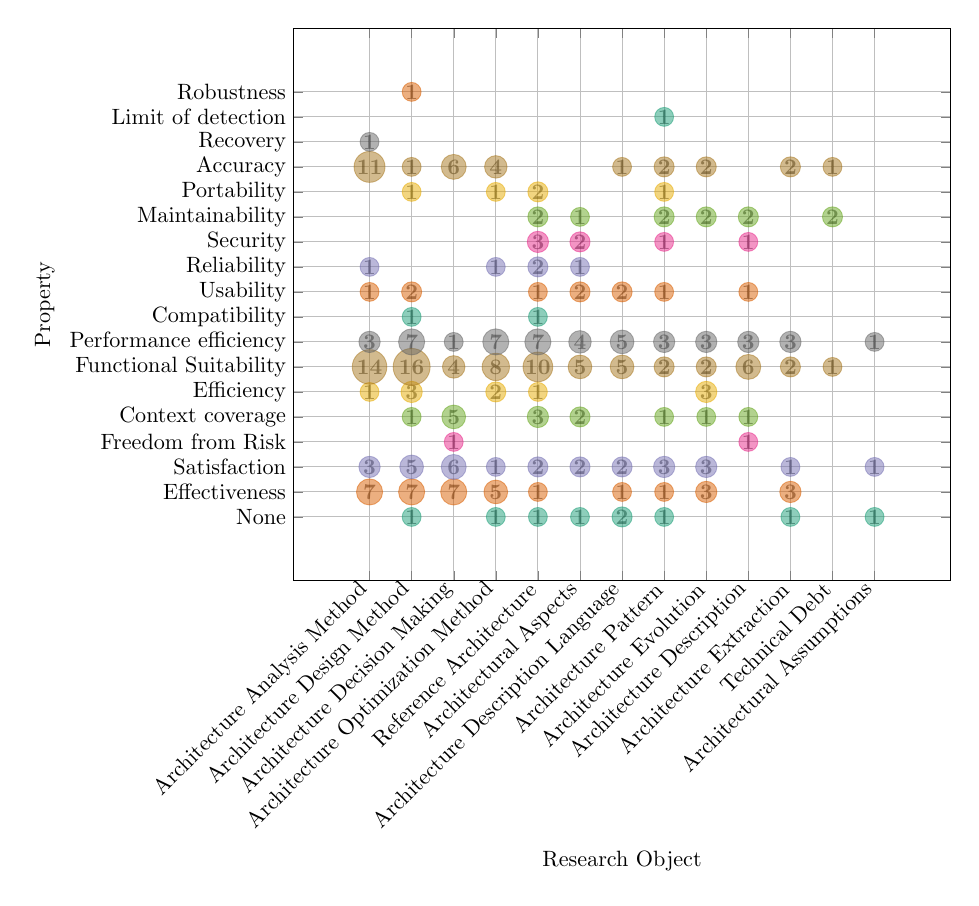
\begin{tikzpicture}[scale=.8]
\pgfplotsset{cycle list/Dark2}
\begin{axis}[width=.99\linewidth,
    enlargelimits=0.15,
    x tick label style={rotate=45,anchor=east},
    xtick={0,1,2,3,4,5,6,7,8,9,10,11,12}, xticklabels={Architecture Analysis Method,Architecture Design Method,Architecture Decision Making,Architecture Optimization Method,Reference Architecture,Architectural Aspects,Architecture Description Language,Architecture Pattern,Architecture Evolution,Architecture Description,Architecture Extraction,Technical Debt,Architectural Assumptions},
    xlabel={Research Object},
    ytick={0,1,2,3,4,5,6,7,8,9,10,11,12,13,14,15,16,17}, yticklabels={None,Effectiveness,Satisfaction,Freedom from Risk,Context coverage,Efficiency,Functional Suitability,Performance efficiency,Compatibility,Usability,Reliability,Security,Maintainability,Portability,Accuracy,Recovery,Limit of detection,Robustness},
    ylabel={Property},
    grid=both,
    scatter,scatter src=y,
    scatter/classes={0={draw=Dark2-A,fill=Dark2-A}, 1={draw=Dark2-B,fill=Dark2-B}, 2={draw=Dark2-C,fill=Dark2-C}, 3={draw=Dark2-D,fill=Dark2-D}, 4={draw=Dark2-E,fill=Dark2-E}, 5={draw=Dark2-F,fill=Dark2-F}, 6={draw=Dark2-G,fill=Dark2-G}, 7={draw=Dark2-H,fill=Dark2-H}, 8={draw=Dark2-A,fill=Dark2-A}, 9={draw=Dark2-B,fill=Dark2-B}, 10={draw=Dark2-C,fill=Dark2-C}, 11={draw=Dark2-D,fill=Dark2-D}, 12={draw=Dark2-E,fill=Dark2-E}, 13={draw=Dark2-F,fill=Dark2-F}, 14={draw=Dark2-G,fill=Dark2-G}, 15={draw=Dark2-H,fill=Dark2-H}, 16={draw=Dark2-A,fill=Dark2-A}, 17={draw=Dark2-B,fill=Dark2-B}}
]

\addplot+[mark=*,mark size=5.905,opacity=0.5,text=black] coordinates { (0,1) } node[text=black,font=\bfseries] {7};
\addplot+[mark=*,mark size=4.816,opacity=0.5,text=black] coordinates { (0,2) } node[text=black,font=\bfseries] {3};
\addplot+[mark=*,mark size=4.272,opacity=0.5,text=black] coordinates { (0,5) } node[text=black,font=\bfseries] {1};
\addplot+[mark=*,mark size=7.810,opacity=0.5,text=black] coordinates { (0,6) } node[text=black,font=\bfseries] {14};
\addplot+[mark=*,mark size=4.816,opacity=0.5,text=black] coordinates { (0,7) } node[text=black,font=\bfseries] {3};
\addplot+[mark=*,mark size=4.272,opacity=0.5,text=black] coordinates { (0,9) } node[text=black,font=\bfseries] {1};
\addplot+[mark=*,mark size=4.272,opacity=0.5,text=black] coordinates { (0,10) } node[text=black,font=\bfseries] {1};
\addplot+[mark=*,mark size=6.993,opacity=0.5,text=black] coordinates { (0,14) } node[text=black,font=\bfseries] {11};
\addplot+[mark=*,mark size=4.272,opacity=0.5,text=black] coordinates { (0,15) } node[text=black,font=\bfseries] {1};
\addplot+[mark=*,mark size=4.272,opacity=0.5,text=black] coordinates { (1,0) } node[text=black,font=\bfseries] {1};
\addplot+[mark=*,mark size=5.905,opacity=0.5,text=black] coordinates { (1,1) } node[text=black,font=\bfseries] {7};
\addplot+[mark=*,mark size=5.361,opacity=0.5,text=black] coordinates { (1,2) } node[text=black,font=\bfseries] {5};
\addplot+[mark=*,mark size=4.272,opacity=0.5,text=black] coordinates { (1,4) } node[text=black,font=\bfseries] {1};
\addplot+[mark=*,mark size=4.816,opacity=0.5,text=black] coordinates { (1,5) } node[text=black,font=\bfseries] {3};
\addplot+[mark=*,mark size=8.354,opacity=0.5,text=black] coordinates { (1,6) } node[text=black,font=\bfseries] {16};
\addplot+[mark=*,mark size=5.905,opacity=0.5,text=black] coordinates { (1,7) } node[text=black,font=\bfseries] {7};
\addplot+[mark=*,mark size=4.272,opacity=0.5,text=black] coordinates { (1,8) } node[text=black,font=\bfseries] {1};
\addplot+[mark=*,mark size=4.544,opacity=0.5,text=black] coordinates { (1,9) } node[text=black,font=\bfseries] {2};
\addplot+[mark=*,mark size=4.272,opacity=0.5,text=black] coordinates { (1,13) } node[text=black,font=\bfseries] {1};
\addplot+[mark=*,mark size=4.272,opacity=0.5,text=black] coordinates { (1,14) } node[text=black,font=\bfseries] {1};
\addplot+[mark=*,mark size=4.272,opacity=0.5,text=black] coordinates { (1,17) } node[text=black,font=\bfseries] {1};
\addplot+[mark=*,mark size=5.905,opacity=0.5,text=black] coordinates { (2,1) } node[text=black,font=\bfseries] {7};
\addplot+[mark=*,mark size=5.633,opacity=0.5,text=black] coordinates { (2,2) } node[text=black,font=\bfseries] {6};
\addplot+[mark=*,mark size=4.272,opacity=0.5,text=black] coordinates { (2,3) } node[text=black,font=\bfseries] {1};
\addplot+[mark=*,mark size=5.361,opacity=0.5,text=black] coordinates { (2,4) } node[text=black,font=\bfseries] {5};
\addplot+[mark=*,mark size=5.088,opacity=0.5,text=black] coordinates { (2,6) } node[text=black,font=\bfseries] {4};
\addplot+[mark=*,mark size=4.272,opacity=0.5,text=black] coordinates { (2,7) } node[text=black,font=\bfseries] {1};
\addplot+[mark=*,mark size=5.633,opacity=0.5,text=black] coordinates { (2,14) } node[text=black,font=\bfseries] {6};
\addplot+[mark=*,mark size=4.272,opacity=0.5,text=black] coordinates { (3,0) } node[text=black,font=\bfseries] {1};
\addplot+[mark=*,mark size=5.361,opacity=0.5,text=black] coordinates { (3,1) } node[text=black,font=\bfseries] {5};
\addplot+[mark=*,mark size=4.272,opacity=0.5,text=black] coordinates { (3,2) } node[text=black,font=\bfseries] {1};
\addplot+[mark=*,mark size=4.544,opacity=0.5,text=black] coordinates { (3,5) } node[text=black,font=\bfseries] {2};
\addplot+[mark=*,mark size=6.177,opacity=0.5,text=black] coordinates { (3,6) } node[text=black,font=\bfseries] {8};
\addplot+[mark=*,mark size=5.905,opacity=0.5,text=black] coordinates { (3,7) } node[text=black,font=\bfseries] {7};
\addplot+[mark=*,mark size=4.272,opacity=0.5,text=black] coordinates { (3,10) } node[text=black,font=\bfseries] {1};
\addplot+[mark=*,mark size=4.272,opacity=0.5,text=black] coordinates { (3,13) } node[text=black,font=\bfseries] {1};
\addplot+[mark=*,mark size=5.088,opacity=0.5,text=black] coordinates { (3,14) } node[text=black,font=\bfseries] {4};
\addplot+[mark=*,mark size=4.272,opacity=0.5,text=black] coordinates { (4,0) } node[text=black,font=\bfseries] {1};
\addplot+[mark=*,mark size=4.272,opacity=0.5,text=black] coordinates { (4,1) } node[text=black,font=\bfseries] {1};
\addplot+[mark=*,mark size=4.544,opacity=0.5,text=black] coordinates { (4,2) } node[text=black,font=\bfseries] {2};
\addplot+[mark=*,mark size=4.816,opacity=0.5,text=black] coordinates { (4,4) } node[text=black,font=\bfseries] {3};
\addplot+[mark=*,mark size=4.272,opacity=0.5,text=black] coordinates { (4,5) } node[text=black,font=\bfseries] {1};
\addplot+[mark=*,mark size=6.721,opacity=0.5,text=black] coordinates { (4,6) } node[text=black,font=\bfseries] {10};
\addplot+[mark=*,mark size=5.905,opacity=0.5,text=black] coordinates { (4,7) } node[text=black,font=\bfseries] {7};
\addplot+[mark=*,mark size=4.272,opacity=0.5,text=black] coordinates { (4,8) } node[text=black,font=\bfseries] {1};
\addplot+[mark=*,mark size=4.272,opacity=0.5,text=black] coordinates { (4,9) } node[text=black,font=\bfseries] {1};
\addplot+[mark=*,mark size=4.544,opacity=0.5,text=black] coordinates { (4,10) } node[text=black,font=\bfseries] {2};
\addplot+[mark=*,mark size=4.816,opacity=0.5,text=black] coordinates { (4,11) } node[text=black,font=\bfseries] {3};
\addplot+[mark=*,mark size=4.544,opacity=0.5,text=black] coordinates { (4,12) } node[text=black,font=\bfseries] {2};
\addplot+[mark=*,mark size=4.544,opacity=0.5,text=black] coordinates { (4,13) } node[text=black,font=\bfseries] {2};
\addplot+[mark=*,mark size=4.272,opacity=0.5,text=black] coordinates { (5,0) } node[text=black,font=\bfseries] {1};
\addplot+[mark=*,mark size=4.544,opacity=0.5,text=black] coordinates { (5,2) } node[text=black,font=\bfseries] {2};
\addplot+[mark=*,mark size=4.544,opacity=0.5,text=black] coordinates { (5,4) } node[text=black,font=\bfseries] {2};
\addplot+[mark=*,mark size=5.361,opacity=0.5,text=black] coordinates { (5,6) } node[text=black,font=\bfseries] {5};
\addplot+[mark=*,mark size=5.088,opacity=0.5,text=black] coordinates { (5,7) } node[text=black,font=\bfseries] {4};
\addplot+[mark=*,mark size=4.544,opacity=0.5,text=black] coordinates { (5,9) } node[text=black,font=\bfseries] {2};
\addplot+[mark=*,mark size=4.272,opacity=0.5,text=black] coordinates { (5,10) } node[text=black,font=\bfseries] {1};
\addplot+[mark=*,mark size=4.544,opacity=0.5,text=black] coordinates { (5,11) } node[text=black,font=\bfseries] {2};
\addplot+[mark=*,mark size=4.272,opacity=0.5,text=black] coordinates { (5,12) } node[text=black,font=\bfseries] {1};
\addplot+[mark=*,mark size=4.544,opacity=0.5,text=black] coordinates { (6,0) } node[text=black,font=\bfseries] {2};
\addplot+[mark=*,mark size=4.272,opacity=0.5,text=black] coordinates { (6,1) } node[text=black,font=\bfseries] {1};
\addplot+[mark=*,mark size=4.544,opacity=0.5,text=black] coordinates { (6,2) } node[text=black,font=\bfseries] {2};
\addplot+[mark=*,mark size=5.361,opacity=0.5,text=black] coordinates { (6,6) } node[text=black,font=\bfseries] {5};
\addplot+[mark=*,mark size=5.361,opacity=0.5,text=black] coordinates { (6,7) } node[text=black,font=\bfseries] {5};
\addplot+[mark=*,mark size=4.544,opacity=0.5,text=black] coordinates { (6,9) } node[text=black,font=\bfseries] {2};
\addplot+[mark=*,mark size=4.272,opacity=0.5,text=black] coordinates { (6,14) } node[text=black,font=\bfseries] {1};
\addplot+[mark=*,mark size=4.272,opacity=0.5,text=black] coordinates { (7,0) } node[text=black,font=\bfseries] {1};
\addplot+[mark=*,mark size=4.272,opacity=0.5,text=black] coordinates { (7,1) } node[text=black,font=\bfseries] {1};
\addplot+[mark=*,mark size=4.816,opacity=0.5,text=black] coordinates { (7,2) } node[text=black,font=\bfseries] {3};
\addplot+[mark=*,mark size=4.272,opacity=0.5,text=black] coordinates { (7,4) } node[text=black,font=\bfseries] {1};
\addplot+[mark=*,mark size=4.544,opacity=0.5,text=black] coordinates { (7,6) } node[text=black,font=\bfseries] {2};
\addplot+[mark=*,mark size=4.816,opacity=0.5,text=black] coordinates { (7,7) } node[text=black,font=\bfseries] {3};
\addplot+[mark=*,mark size=4.272,opacity=0.5,text=black] coordinates { (7,9) } node[text=black,font=\bfseries] {1};
\addplot+[mark=*,mark size=4.272,opacity=0.5,text=black] coordinates { (7,11) } node[text=black,font=\bfseries] {1};
\addplot+[mark=*,mark size=4.544,opacity=0.5,text=black] coordinates { (7,12) } node[text=black,font=\bfseries] {2};
\addplot+[mark=*,mark size=4.272,opacity=0.5,text=black] coordinates { (7,13) } node[text=black,font=\bfseries] {1};
\addplot+[mark=*,mark size=4.544,opacity=0.5,text=black] coordinates { (7,14) } node[text=black,font=\bfseries] {2};
\addplot+[mark=*,mark size=4.272,opacity=0.5,text=black] coordinates { (7,16) } node[text=black,font=\bfseries] {1};
\addplot+[mark=*,mark size=4.816,opacity=0.5,text=black] coordinates { (8,1) } node[text=black,font=\bfseries] {3};
\addplot+[mark=*,mark size=4.816,opacity=0.5,text=black] coordinates { (8,2) } node[text=black,font=\bfseries] {3};
\addplot+[mark=*,mark size=4.272,opacity=0.5,text=black] coordinates { (8,4) } node[text=black,font=\bfseries] {1};
\addplot+[mark=*,mark size=4.816,opacity=0.5,text=black] coordinates { (8,5) } node[text=black,font=\bfseries] {3};
\addplot+[mark=*,mark size=4.544,opacity=0.5,text=black] coordinates { (8,6) } node[text=black,font=\bfseries] {2};
\addplot+[mark=*,mark size=4.816,opacity=0.5,text=black] coordinates { (8,7) } node[text=black,font=\bfseries] {3};
\addplot+[mark=*,mark size=4.544,opacity=0.5,text=black] coordinates { (8,12) } node[text=black,font=\bfseries] {2};
\addplot+[mark=*,mark size=4.544,opacity=0.5,text=black] coordinates { (8,14) } node[text=black,font=\bfseries] {2};
\addplot+[mark=*,mark size=4.272,opacity=0.5,text=black] coordinates { (9,3) } node[text=black,font=\bfseries] {1};
\addplot+[mark=*,mark size=4.272,opacity=0.5,text=black] coordinates { (9,4) } node[text=black,font=\bfseries] {1};
\addplot+[mark=*,mark size=5.633,opacity=0.5,text=black] coordinates { (9,6) } node[text=black,font=\bfseries] {6};
\addplot+[mark=*,mark size=4.816,opacity=0.5,text=black] coordinates { (9,7) } node[text=black,font=\bfseries] {3};
\addplot+[mark=*,mark size=4.272,opacity=0.5,text=black] coordinates { (9,9) } node[text=black,font=\bfseries] {1};
\addplot+[mark=*,mark size=4.272,opacity=0.5,text=black] coordinates { (9,11) } node[text=black,font=\bfseries] {1};
\addplot+[mark=*,mark size=4.544,opacity=0.5,text=black] coordinates { (9,12) } node[text=black,font=\bfseries] {2};
\addplot+[mark=*,mark size=4.272,opacity=0.5,text=black] coordinates { (10,0) } node[text=black,font=\bfseries] {1};
\addplot+[mark=*,mark size=4.816,opacity=0.5,text=black] coordinates { (10,1) } node[text=black,font=\bfseries] {3};
\addplot+[mark=*,mark size=4.272,opacity=0.5,text=black] coordinates { (10,2) } node[text=black,font=\bfseries] {1};
\addplot+[mark=*,mark size=4.544,opacity=0.5,text=black] coordinates { (10,6) } node[text=black,font=\bfseries] {2};
\addplot+[mark=*,mark size=4.816,opacity=0.5,text=black] coordinates { (10,7) } node[text=black,font=\bfseries] {3};
\addplot+[mark=*,mark size=4.544,opacity=0.5,text=black] coordinates { (10,14) } node[text=black,font=\bfseries] {2};
\addplot+[mark=*,mark size=4.272,opacity=0.5,text=black] coordinates { (11,6) } node[text=black,font=\bfseries] {1};
\addplot+[mark=*,mark size=4.544,opacity=0.5,text=black] coordinates { (11,12) } node[text=black,font=\bfseries] {2};
\addplot+[mark=*,mark size=4.272,opacity=0.5,text=black] coordinates { (11,14) } node[text=black,font=\bfseries] {1};
\addplot+[mark=*,mark size=4.272,opacity=0.5,text=black] coordinates { (12,0) } node[text=black,font=\bfseries] {1};
\addplot+[mark=*,mark size=4.272,opacity=0.5,text=black] coordinates { (12,2) } node[text=black,font=\bfseries] {1};
\addplot+[mark=*,mark size=4.272,opacity=0.5,text=black] coordinates { (12,7) } node[text=black,font=\bfseries] {1};


\end{axis}
\end{tikzpicture}
\end{center}
%\caption{Portfolio f\"ur Research Object und Property (Gr\"o\ss{}e entspricht der Anzahl)}\label{fig:port_researchobject_property}
%\end{figure}


%\subsection{Portfolio f\"ur Property und Research Object (Gr\"o\ss{}e entspricht der Anzahl)}
%\begin{figure}
\begin{center}
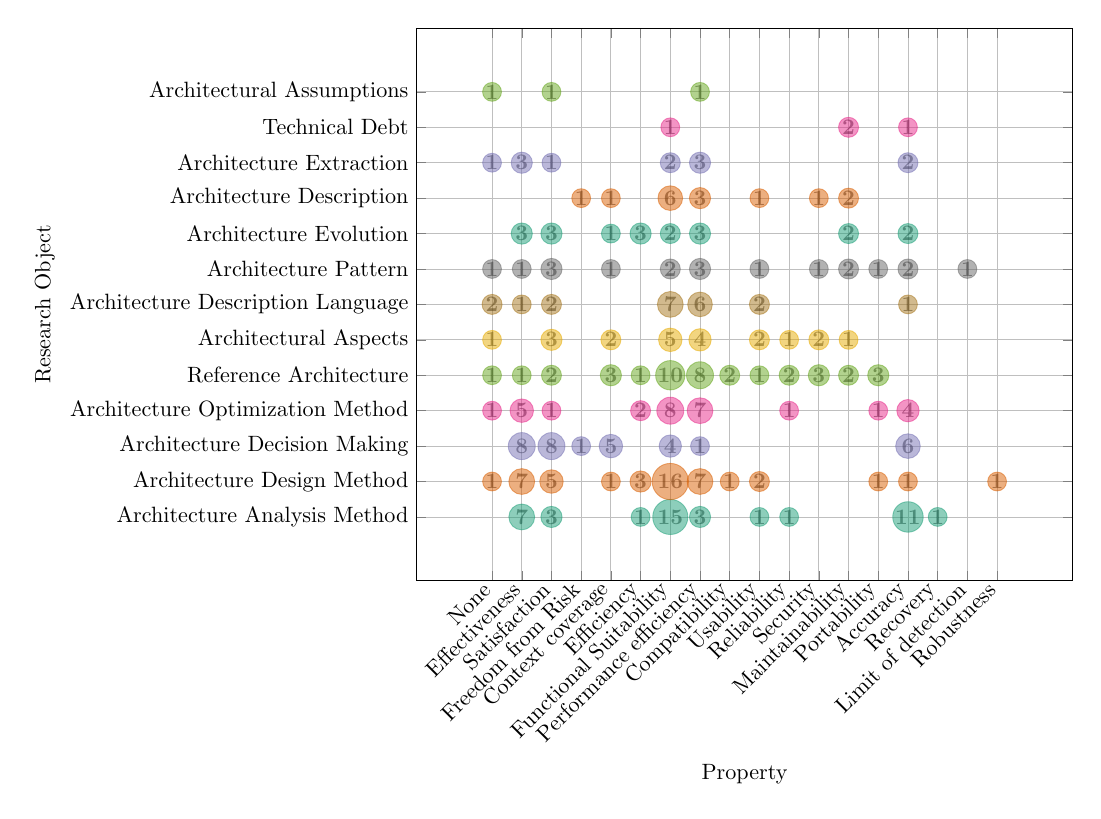
\begin{tikzpicture}[scale=.8]
\pgfplotsset{cycle list/Dark2}
\begin{axis}[width=.99\linewidth,
    enlargelimits=0.15,
    x tick label style={rotate=45,anchor=east},
    xtick={0,1,2,3,4,5,6,7,8,9,10,11,12,13,14,15,16,17}, xticklabels={None,Effectiveness,Satisfaction,Freedom from Risk,Context coverage,Efficiency,Functional Suitability,Performance efficiency,Compatibility,Usability,Reliability,Security,Maintainability,Portability,Accuracy,Recovery,Limit of detection,Robustness},
    xlabel={Property},
    ytick={0,1,2,3,4,5,6,7,8,9,10,11,12}, yticklabels={Architecture Analysis Method,Architecture Design Method,Architecture Decision Making,Architecture Optimization Method,Reference Architecture,Architectural Aspects,Architecture Description Language,Architecture Pattern,Architecture Evolution,Architecture Description,Architecture Extraction,Technical Debt,Architectural Assumptions},
    ylabel={Research Object},
    grid=both,
    scatter,scatter src=y,
    scatter/classes={0={draw=Dark2-A,fill=Dark2-A}, 1={draw=Dark2-B,fill=Dark2-B}, 2={draw=Dark2-C,fill=Dark2-C}, 3={draw=Dark2-D,fill=Dark2-D}, 4={draw=Dark2-E,fill=Dark2-E}, 5={draw=Dark2-F,fill=Dark2-F}, 6={draw=Dark2-G,fill=Dark2-G}, 7={draw=Dark2-H,fill=Dark2-H}, 8={draw=Dark2-A,fill=Dark2-A}, 9={draw=Dark2-B,fill=Dark2-B}, 10={draw=Dark2-C,fill=Dark2-C}, 11={draw=Dark2-D,fill=Dark2-D}, 12={draw=Dark2-E,fill=Dark2-E}}
]

\addplot+[mark=*,mark size=4.262,opacity=0.5,text=black] coordinates { (0,1) } node[text=black,font=\bfseries] {1};
\addplot+[mark=*,mark size=4.262,opacity=0.5,text=black] coordinates { (0,3) } node[text=black,font=\bfseries] {1};
\addplot+[mark=*,mark size=4.262,opacity=0.5,text=black] coordinates { (0,4) } node[text=black,font=\bfseries] {1};
\addplot+[mark=*,mark size=4.262,opacity=0.5,text=black] coordinates { (0,5) } node[text=black,font=\bfseries] {1};
\addplot+[mark=*,mark size=4.525,opacity=0.5,text=black] coordinates { (0,6) } node[text=black,font=\bfseries] {2};
\addplot+[mark=*,mark size=4.262,opacity=0.5,text=black] coordinates { (0,7) } node[text=black,font=\bfseries] {1};
\addplot+[mark=*,mark size=4.262,opacity=0.5,text=black] coordinates { (0,10) } node[text=black,font=\bfseries] {1};
\addplot+[mark=*,mark size=4.262,opacity=0.5,text=black] coordinates { (0,12) } node[text=black,font=\bfseries] {1};
\addplot+[mark=*,mark size=5.836,opacity=0.5,text=black] coordinates { (1,0) } node[text=black,font=\bfseries] {7};
\addplot+[mark=*,mark size=5.836,opacity=0.5,text=black] coordinates { (1,1) } node[text=black,font=\bfseries] {7};
\addplot+[mark=*,mark size=6.098,opacity=0.5,text=black] coordinates { (1,2) } node[text=black,font=\bfseries] {8};
\addplot+[mark=*,mark size=5.311,opacity=0.5,text=black] coordinates { (1,3) } node[text=black,font=\bfseries] {5};
\addplot+[mark=*,mark size=4.262,opacity=0.5,text=black] coordinates { (1,4) } node[text=black,font=\bfseries] {1};
\addplot+[mark=*,mark size=4.262,opacity=0.5,text=black] coordinates { (1,6) } node[text=black,font=\bfseries] {1};
\addplot+[mark=*,mark size=4.262,opacity=0.5,text=black] coordinates { (1,7) } node[text=black,font=\bfseries] {1};
\addplot+[mark=*,mark size=4.787,opacity=0.5,text=black] coordinates { (1,8) } node[text=black,font=\bfseries] {3};
\addplot+[mark=*,mark size=4.787,opacity=0.5,text=black] coordinates { (1,10) } node[text=black,font=\bfseries] {3};
\addplot+[mark=*,mark size=4.787,opacity=0.5,text=black] coordinates { (2,0) } node[text=black,font=\bfseries] {3};
\addplot+[mark=*,mark size=5.311,opacity=0.5,text=black] coordinates { (2,1) } node[text=black,font=\bfseries] {5};
\addplot+[mark=*,mark size=6.098,opacity=0.5,text=black] coordinates { (2,2) } node[text=black,font=\bfseries] {8};
\addplot+[mark=*,mark size=4.262,opacity=0.5,text=black] coordinates { (2,3) } node[text=black,font=\bfseries] {1};
\addplot+[mark=*,mark size=4.525,opacity=0.5,text=black] coordinates { (2,4) } node[text=black,font=\bfseries] {2};
\addplot+[mark=*,mark size=4.787,opacity=0.5,text=black] coordinates { (2,5) } node[text=black,font=\bfseries] {3};
\addplot+[mark=*,mark size=4.525,opacity=0.5,text=black] coordinates { (2,6) } node[text=black,font=\bfseries] {2};
\addplot+[mark=*,mark size=4.787,opacity=0.5,text=black] coordinates { (2,7) } node[text=black,font=\bfseries] {3};
\addplot+[mark=*,mark size=4.787,opacity=0.5,text=black] coordinates { (2,8) } node[text=black,font=\bfseries] {3};
\addplot+[mark=*,mark size=4.262,opacity=0.5,text=black] coordinates { (2,10) } node[text=black,font=\bfseries] {1};
\addplot+[mark=*,mark size=4.262,opacity=0.5,text=black] coordinates { (2,12) } node[text=black,font=\bfseries] {1};
\addplot+[mark=*,mark size=4.262,opacity=0.5,text=black] coordinates { (3,2) } node[text=black,font=\bfseries] {1};
\addplot+[mark=*,mark size=4.262,opacity=0.5,text=black] coordinates { (3,9) } node[text=black,font=\bfseries] {1};
\addplot+[mark=*,mark size=4.262,opacity=0.5,text=black] coordinates { (4,1) } node[text=black,font=\bfseries] {1};
\addplot+[mark=*,mark size=5.311,opacity=0.5,text=black] coordinates { (4,2) } node[text=black,font=\bfseries] {5};
\addplot+[mark=*,mark size=4.787,opacity=0.5,text=black] coordinates { (4,4) } node[text=black,font=\bfseries] {3};
\addplot+[mark=*,mark size=4.525,opacity=0.5,text=black] coordinates { (4,5) } node[text=black,font=\bfseries] {2};
\addplot+[mark=*,mark size=4.262,opacity=0.5,text=black] coordinates { (4,7) } node[text=black,font=\bfseries] {1};
\addplot+[mark=*,mark size=4.262,opacity=0.5,text=black] coordinates { (4,8) } node[text=black,font=\bfseries] {1};
\addplot+[mark=*,mark size=4.262,opacity=0.5,text=black] coordinates { (4,9) } node[text=black,font=\bfseries] {1};
\addplot+[mark=*,mark size=4.262,opacity=0.5,text=black] coordinates { (5,0) } node[text=black,font=\bfseries] {1};
\addplot+[mark=*,mark size=4.787,opacity=0.5,text=black] coordinates { (5,1) } node[text=black,font=\bfseries] {3};
\addplot+[mark=*,mark size=4.525,opacity=0.5,text=black] coordinates { (5,3) } node[text=black,font=\bfseries] {2};
\addplot+[mark=*,mark size=4.262,opacity=0.5,text=black] coordinates { (5,4) } node[text=black,font=\bfseries] {1};
\addplot+[mark=*,mark size=4.787,opacity=0.5,text=black] coordinates { (5,8) } node[text=black,font=\bfseries] {3};
\addplot+[mark=*,mark size=7.934,opacity=0.5,text=black] coordinates { (6,0) } node[text=black,font=\bfseries] {15};
\addplot+[mark=*,mark size=8.197,opacity=0.5,text=black] coordinates { (6,1) } node[text=black,font=\bfseries] {16};
\addplot+[mark=*,mark size=5.049,opacity=0.5,text=black] coordinates { (6,2) } node[text=black,font=\bfseries] {4};
\addplot+[mark=*,mark size=6.098,opacity=0.5,text=black] coordinates { (6,3) } node[text=black,font=\bfseries] {8};
\addplot+[mark=*,mark size=6.623,opacity=0.5,text=black] coordinates { (6,4) } node[text=black,font=\bfseries] {10};
\addplot+[mark=*,mark size=5.311,opacity=0.5,text=black] coordinates { (6,5) } node[text=black,font=\bfseries] {5};
\addplot+[mark=*,mark size=5.836,opacity=0.5,text=black] coordinates { (6,6) } node[text=black,font=\bfseries] {7};
\addplot+[mark=*,mark size=4.525,opacity=0.5,text=black] coordinates { (6,7) } node[text=black,font=\bfseries] {2};
\addplot+[mark=*,mark size=4.525,opacity=0.5,text=black] coordinates { (6,8) } node[text=black,font=\bfseries] {2};
\addplot+[mark=*,mark size=5.574,opacity=0.5,text=black] coordinates { (6,9) } node[text=black,font=\bfseries] {6};
\addplot+[mark=*,mark size=4.525,opacity=0.5,text=black] coordinates { (6,10) } node[text=black,font=\bfseries] {2};
\addplot+[mark=*,mark size=4.262,opacity=0.5,text=black] coordinates { (6,11) } node[text=black,font=\bfseries] {1};
\addplot+[mark=*,mark size=4.787,opacity=0.5,text=black] coordinates { (7,0) } node[text=black,font=\bfseries] {3};
\addplot+[mark=*,mark size=5.836,opacity=0.5,text=black] coordinates { (7,1) } node[text=black,font=\bfseries] {7};
\addplot+[mark=*,mark size=4.262,opacity=0.5,text=black] coordinates { (7,2) } node[text=black,font=\bfseries] {1};
\addplot+[mark=*,mark size=5.836,opacity=0.5,text=black] coordinates { (7,3) } node[text=black,font=\bfseries] {7};
\addplot+[mark=*,mark size=6.098,opacity=0.5,text=black] coordinates { (7,4) } node[text=black,font=\bfseries] {8};
\addplot+[mark=*,mark size=5.049,opacity=0.5,text=black] coordinates { (7,5) } node[text=black,font=\bfseries] {4};
\addplot+[mark=*,mark size=5.574,opacity=0.5,text=black] coordinates { (7,6) } node[text=black,font=\bfseries] {6};
\addplot+[mark=*,mark size=4.787,opacity=0.5,text=black] coordinates { (7,7) } node[text=black,font=\bfseries] {3};
\addplot+[mark=*,mark size=4.787,opacity=0.5,text=black] coordinates { (7,8) } node[text=black,font=\bfseries] {3};
\addplot+[mark=*,mark size=4.787,opacity=0.5,text=black] coordinates { (7,9) } node[text=black,font=\bfseries] {3};
\addplot+[mark=*,mark size=4.787,opacity=0.5,text=black] coordinates { (7,10) } node[text=black,font=\bfseries] {3};
\addplot+[mark=*,mark size=4.262,opacity=0.5,text=black] coordinates { (7,12) } node[text=black,font=\bfseries] {1};
\addplot+[mark=*,mark size=4.262,opacity=0.5,text=black] coordinates { (8,1) } node[text=black,font=\bfseries] {1};
\addplot+[mark=*,mark size=4.525,opacity=0.5,text=black] coordinates { (8,4) } node[text=black,font=\bfseries] {2};
\addplot+[mark=*,mark size=4.262,opacity=0.5,text=black] coordinates { (9,0) } node[text=black,font=\bfseries] {1};
\addplot+[mark=*,mark size=4.525,opacity=0.5,text=black] coordinates { (9,1) } node[text=black,font=\bfseries] {2};
\addplot+[mark=*,mark size=4.262,opacity=0.5,text=black] coordinates { (9,4) } node[text=black,font=\bfseries] {1};
\addplot+[mark=*,mark size=4.525,opacity=0.5,text=black] coordinates { (9,5) } node[text=black,font=\bfseries] {2};
\addplot+[mark=*,mark size=4.525,opacity=0.5,text=black] coordinates { (9,6) } node[text=black,font=\bfseries] {2};
\addplot+[mark=*,mark size=4.262,opacity=0.5,text=black] coordinates { (9,7) } node[text=black,font=\bfseries] {1};
\addplot+[mark=*,mark size=4.262,opacity=0.5,text=black] coordinates { (9,9) } node[text=black,font=\bfseries] {1};
\addplot+[mark=*,mark size=4.262,opacity=0.5,text=black] coordinates { (10,0) } node[text=black,font=\bfseries] {1};
\addplot+[mark=*,mark size=4.262,opacity=0.5,text=black] coordinates { (10,3) } node[text=black,font=\bfseries] {1};
\addplot+[mark=*,mark size=4.525,opacity=0.5,text=black] coordinates { (10,4) } node[text=black,font=\bfseries] {2};
\addplot+[mark=*,mark size=4.262,opacity=0.5,text=black] coordinates { (10,5) } node[text=black,font=\bfseries] {1};
\addplot+[mark=*,mark size=4.787,opacity=0.5,text=black] coordinates { (11,4) } node[text=black,font=\bfseries] {3};
\addplot+[mark=*,mark size=4.525,opacity=0.5,text=black] coordinates { (11,5) } node[text=black,font=\bfseries] {2};
\addplot+[mark=*,mark size=4.262,opacity=0.5,text=black] coordinates { (11,7) } node[text=black,font=\bfseries] {1};
\addplot+[mark=*,mark size=4.262,opacity=0.5,text=black] coordinates { (11,9) } node[text=black,font=\bfseries] {1};
\addplot+[mark=*,mark size=4.525,opacity=0.5,text=black] coordinates { (12,4) } node[text=black,font=\bfseries] {2};
\addplot+[mark=*,mark size=4.262,opacity=0.5,text=black] coordinates { (12,5) } node[text=black,font=\bfseries] {1};
\addplot+[mark=*,mark size=4.525,opacity=0.5,text=black] coordinates { (12,7) } node[text=black,font=\bfseries] {2};
\addplot+[mark=*,mark size=4.525,opacity=0.5,text=black] coordinates { (12,8) } node[text=black,font=\bfseries] {2};
\addplot+[mark=*,mark size=4.525,opacity=0.5,text=black] coordinates { (12,9) } node[text=black,font=\bfseries] {2};
\addplot+[mark=*,mark size=4.525,opacity=0.5,text=black] coordinates { (12,11) } node[text=black,font=\bfseries] {2};
\addplot+[mark=*,mark size=4.262,opacity=0.5,text=black] coordinates { (13,1) } node[text=black,font=\bfseries] {1};
\addplot+[mark=*,mark size=4.262,opacity=0.5,text=black] coordinates { (13,3) } node[text=black,font=\bfseries] {1};
\addplot+[mark=*,mark size=4.787,opacity=0.5,text=black] coordinates { (13,4) } node[text=black,font=\bfseries] {3};
\addplot+[mark=*,mark size=4.262,opacity=0.5,text=black] coordinates { (13,7) } node[text=black,font=\bfseries] {1};
\addplot+[mark=*,mark size=6.885,opacity=0.5,text=black] coordinates { (14,0) } node[text=black,font=\bfseries] {11};
\addplot+[mark=*,mark size=4.262,opacity=0.5,text=black] coordinates { (14,1) } node[text=black,font=\bfseries] {1};
\addplot+[mark=*,mark size=5.574,opacity=0.5,text=black] coordinates { (14,2) } node[text=black,font=\bfseries] {6};
\addplot+[mark=*,mark size=5.049,opacity=0.5,text=black] coordinates { (14,3) } node[text=black,font=\bfseries] {4};
\addplot+[mark=*,mark size=4.262,opacity=0.5,text=black] coordinates { (14,6) } node[text=black,font=\bfseries] {1};
\addplot+[mark=*,mark size=4.525,opacity=0.5,text=black] coordinates { (14,7) } node[text=black,font=\bfseries] {2};
\addplot+[mark=*,mark size=4.525,opacity=0.5,text=black] coordinates { (14,8) } node[text=black,font=\bfseries] {2};
\addplot+[mark=*,mark size=4.525,opacity=0.5,text=black] coordinates { (14,10) } node[text=black,font=\bfseries] {2};
\addplot+[mark=*,mark size=4.262,opacity=0.5,text=black] coordinates { (14,11) } node[text=black,font=\bfseries] {1};
\addplot+[mark=*,mark size=4.262,opacity=0.5,text=black] coordinates { (15,0) } node[text=black,font=\bfseries] {1};
\addplot+[mark=*,mark size=4.262,opacity=0.5,text=black] coordinates { (16,7) } node[text=black,font=\bfseries] {1};
\addplot+[mark=*,mark size=4.262,opacity=0.5,text=black] coordinates { (17,1) } node[text=black,font=\bfseries] {1};


\end{axis}
\end{tikzpicture}
\end{center}
%\caption{Portfolio f\"ur Property und Research Object (Gr\"o\ss{}e entspricht der Anzahl)}\label{fig:port_property_researchobject}
%\end{figure}




\section{Property vs. Evaluation Methods}

%\subsection{Portfolio f\"ur Property und Evaluation Method (Gr\"o\ss{}e entspricht der Anzahl)}
%\begin{figure}
\begin{center}
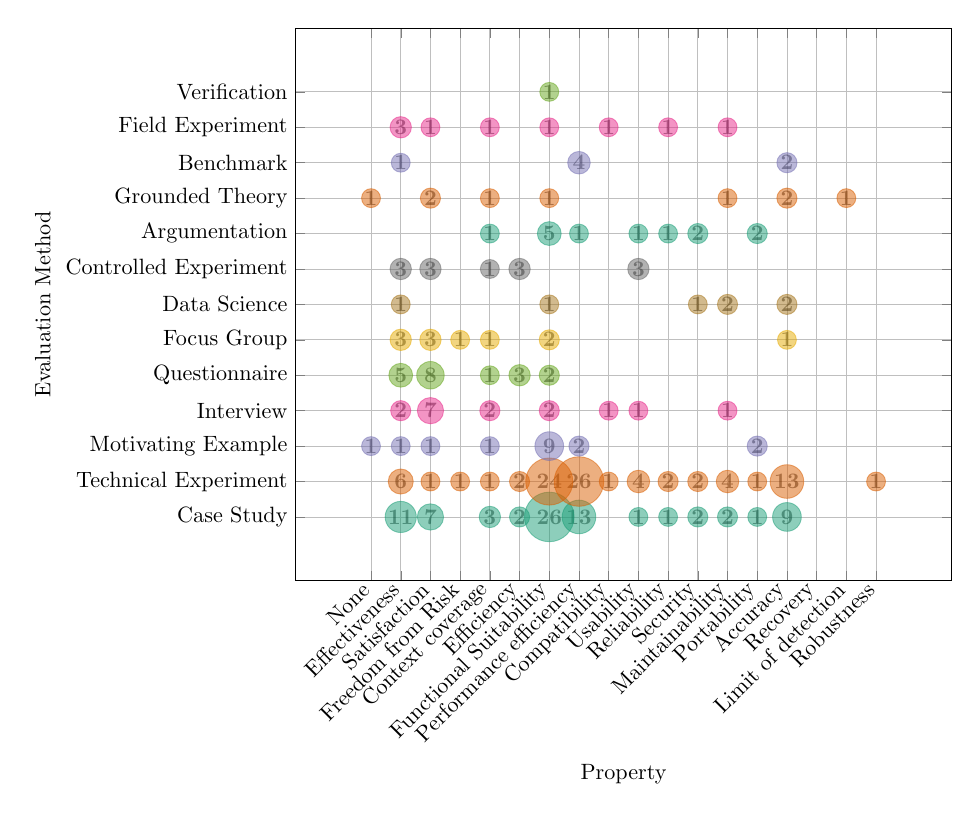
\begin{tikzpicture}[scale=.8]
\pgfplotsset{cycle list/Dark2}
\begin{axis}[width=.99\linewidth,
    enlargelimits=0.15,
    x tick label style={rotate=45,anchor=east},
    xtick={0,1,2,3,4,5,6,7,8,9,10,11,12,13,14,15,16,17}, xticklabels={None,Effectiveness,Satisfaction,Freedom from Risk,Context coverage,Efficiency,Functional Suitability,Performance efficiency,Compatibility,Usability,Reliability,Security,Maintainability,Portability,Accuracy,Recovery,Limit of detection,Robustness},
    xlabel={Property},
    ytick={0,1,2,3,4,5,6,7,8,9,10,11,12}, yticklabels={Case Study,Technical Experiment,Motivating Example,Interview,Questionnaire,Focus Group,Data Science,Controlled Experiment,Argumentation,Grounded Theory,Benchmark,Field Experiment,Verification},
    ylabel={Evaluation Method},
    grid=both,
    scatter,scatter src=y,
    scatter/classes={0={draw=Dark2-A,fill=Dark2-A}, 1={draw=Dark2-B,fill=Dark2-B}, 2={draw=Dark2-C,fill=Dark2-C}, 3={draw=Dark2-D,fill=Dark2-D}, 4={draw=Dark2-E,fill=Dark2-E}, 5={draw=Dark2-F,fill=Dark2-F}, 6={draw=Dark2-G,fill=Dark2-G}, 7={draw=Dark2-H,fill=Dark2-H}, 8={draw=Dark2-A,fill=Dark2-A}, 9={draw=Dark2-B,fill=Dark2-B}, 10={draw=Dark2-C,fill=Dark2-C}, 11={draw=Dark2-D,fill=Dark2-D}, 12={draw=Dark2-E,fill=Dark2-E}}
]

\addplot+[mark=*,mark size=4.277,opacity=0.5,text=black] coordinates { (0,2) } node[text=black,font=\bfseries] {1};
\addplot+[mark=*,mark size=4.277,opacity=0.5,text=black] coordinates { (0,9) } node[text=black,font=\bfseries] {1};
\addplot+[mark=*,mark size=7.045,opacity=0.5,text=black] coordinates { (1,0) } node[text=black,font=\bfseries] {11};
\addplot+[mark=*,mark size=5.661,opacity=0.5,text=black] coordinates { (1,1) } node[text=black,font=\bfseries] {6};
\addplot+[mark=*,mark size=4.277,opacity=0.5,text=black] coordinates { (1,2) } node[text=black,font=\bfseries] {1};
\addplot+[mark=*,mark size=4.554,opacity=0.5,text=black] coordinates { (1,3) } node[text=black,font=\bfseries] {2};
\addplot+[mark=*,mark size=5.384,opacity=0.5,text=black] coordinates { (1,4) } node[text=black,font=\bfseries] {5};
\addplot+[mark=*,mark size=4.830,opacity=0.5,text=black] coordinates { (1,5) } node[text=black,font=\bfseries] {3};
\addplot+[mark=*,mark size=4.277,opacity=0.5,text=black] coordinates { (1,6) } node[text=black,font=\bfseries] {1};
\addplot+[mark=*,mark size=4.830,opacity=0.5,text=black] coordinates { (1,7) } node[text=black,font=\bfseries] {3};
\addplot+[mark=*,mark size=4.277,opacity=0.5,text=black] coordinates { (1,10) } node[text=black,font=\bfseries] {1};
\addplot+[mark=*,mark size=4.830,opacity=0.5,text=black] coordinates { (1,11) } node[text=black,font=\bfseries] {3};
\addplot+[mark=*,mark size=5.938,opacity=0.5,text=black] coordinates { (2,0) } node[text=black,font=\bfseries] {7};
\addplot+[mark=*,mark size=4.277,opacity=0.5,text=black] coordinates { (2,1) } node[text=black,font=\bfseries] {1};
\addplot+[mark=*,mark size=4.277,opacity=0.5,text=black] coordinates { (2,2) } node[text=black,font=\bfseries] {1};
\addplot+[mark=*,mark size=5.938,opacity=0.5,text=black] coordinates { (2,3) } node[text=black,font=\bfseries] {7};
\addplot+[mark=*,mark size=6.215,opacity=0.5,text=black] coordinates { (2,4) } node[text=black,font=\bfseries] {8};
\addplot+[mark=*,mark size=4.830,opacity=0.5,text=black] coordinates { (2,5) } node[text=black,font=\bfseries] {3};
\addplot+[mark=*,mark size=4.830,opacity=0.5,text=black] coordinates { (2,7) } node[text=black,font=\bfseries] {3};
\addplot+[mark=*,mark size=4.554,opacity=0.5,text=black] coordinates { (2,9) } node[text=black,font=\bfseries] {2};
\addplot+[mark=*,mark size=4.277,opacity=0.5,text=black] coordinates { (2,11) } node[text=black,font=\bfseries] {1};
\addplot+[mark=*,mark size=4.277,opacity=0.5,text=black] coordinates { (3,1) } node[text=black,font=\bfseries] {1};
\addplot+[mark=*,mark size=4.277,opacity=0.5,text=black] coordinates { (3,5) } node[text=black,font=\bfseries] {1};
\addplot+[mark=*,mark size=4.830,opacity=0.5,text=black] coordinates { (4,0) } node[text=black,font=\bfseries] {3};
\addplot+[mark=*,mark size=4.277,opacity=0.5,text=black] coordinates { (4,1) } node[text=black,font=\bfseries] {1};
\addplot+[mark=*,mark size=4.277,opacity=0.5,text=black] coordinates { (4,2) } node[text=black,font=\bfseries] {1};
\addplot+[mark=*,mark size=4.554,opacity=0.5,text=black] coordinates { (4,3) } node[text=black,font=\bfseries] {2};
\addplot+[mark=*,mark size=4.277,opacity=0.5,text=black] coordinates { (4,4) } node[text=black,font=\bfseries] {1};
\addplot+[mark=*,mark size=4.277,opacity=0.5,text=black] coordinates { (4,5) } node[text=black,font=\bfseries] {1};
\addplot+[mark=*,mark size=4.277,opacity=0.5,text=black] coordinates { (4,7) } node[text=black,font=\bfseries] {1};
\addplot+[mark=*,mark size=4.277,opacity=0.5,text=black] coordinates { (4,8) } node[text=black,font=\bfseries] {1};
\addplot+[mark=*,mark size=4.277,opacity=0.5,text=black] coordinates { (4,9) } node[text=black,font=\bfseries] {1};
\addplot+[mark=*,mark size=4.277,opacity=0.5,text=black] coordinates { (4,11) } node[text=black,font=\bfseries] {1};
\addplot+[mark=*,mark size=4.554,opacity=0.5,text=black] coordinates { (5,0) } node[text=black,font=\bfseries] {2};
\addplot+[mark=*,mark size=4.554,opacity=0.5,text=black] coordinates { (5,1) } node[text=black,font=\bfseries] {2};
\addplot+[mark=*,mark size=4.830,opacity=0.5,text=black] coordinates { (5,4) } node[text=black,font=\bfseries] {3};
\addplot+[mark=*,mark size=4.830,opacity=0.5,text=black] coordinates { (5,7) } node[text=black,font=\bfseries] {3};
\addplot+[mark=*,mark size=11.197,opacity=0.5,text=black] coordinates { (6,0) } node[text=black,font=\bfseries] {26};
\addplot+[mark=*,mark size=10.644,opacity=0.5,text=black] coordinates { (6,1) } node[text=black,font=\bfseries] {24};
\addplot+[mark=*,mark size=6.491,opacity=0.5,text=black] coordinates { (6,2) } node[text=black,font=\bfseries] {9};
\addplot+[mark=*,mark size=4.554,opacity=0.5,text=black] coordinates { (6,3) } node[text=black,font=\bfseries] {2};
\addplot+[mark=*,mark size=4.554,opacity=0.5,text=black] coordinates { (6,4) } node[text=black,font=\bfseries] {2};
\addplot+[mark=*,mark size=4.554,opacity=0.5,text=black] coordinates { (6,5) } node[text=black,font=\bfseries] {2};
\addplot+[mark=*,mark size=4.277,opacity=0.5,text=black] coordinates { (6,6) } node[text=black,font=\bfseries] {1};
\addplot+[mark=*,mark size=5.384,opacity=0.5,text=black] coordinates { (6,8) } node[text=black,font=\bfseries] {5};
\addplot+[mark=*,mark size=4.277,opacity=0.5,text=black] coordinates { (6,9) } node[text=black,font=\bfseries] {1};
\addplot+[mark=*,mark size=4.277,opacity=0.5,text=black] coordinates { (6,11) } node[text=black,font=\bfseries] {1};
\addplot+[mark=*,mark size=4.277,opacity=0.5,text=black] coordinates { (6,12) } node[text=black,font=\bfseries] {1};
\addplot+[mark=*,mark size=7.599,opacity=0.5,text=black] coordinates { (7,0) } node[text=black,font=\bfseries] {13};
\addplot+[mark=*,mark size=11.197,opacity=0.5,text=black] coordinates { (7,1) } node[text=black,font=\bfseries] {26};
\addplot+[mark=*,mark size=4.554,opacity=0.5,text=black] coordinates { (7,2) } node[text=black,font=\bfseries] {2};
\addplot+[mark=*,mark size=4.277,opacity=0.5,text=black] coordinates { (7,8) } node[text=black,font=\bfseries] {1};
\addplot+[mark=*,mark size=5.107,opacity=0.5,text=black] coordinates { (7,10) } node[text=black,font=\bfseries] {4};
\addplot+[mark=*,mark size=4.277,opacity=0.5,text=black] coordinates { (8,1) } node[text=black,font=\bfseries] {1};
\addplot+[mark=*,mark size=4.277,opacity=0.5,text=black] coordinates { (8,3) } node[text=black,font=\bfseries] {1};
\addplot+[mark=*,mark size=4.277,opacity=0.5,text=black] coordinates { (8,11) } node[text=black,font=\bfseries] {1};
\addplot+[mark=*,mark size=4.277,opacity=0.5,text=black] coordinates { (9,0) } node[text=black,font=\bfseries] {1};
\addplot+[mark=*,mark size=5.107,opacity=0.5,text=black] coordinates { (9,1) } node[text=black,font=\bfseries] {4};
\addplot+[mark=*,mark size=4.277,opacity=0.5,text=black] coordinates { (9,3) } node[text=black,font=\bfseries] {1};
\addplot+[mark=*,mark size=4.830,opacity=0.5,text=black] coordinates { (9,7) } node[text=black,font=\bfseries] {3};
\addplot+[mark=*,mark size=4.277,opacity=0.5,text=black] coordinates { (9,8) } node[text=black,font=\bfseries] {1};
\addplot+[mark=*,mark size=4.277,opacity=0.5,text=black] coordinates { (10,0) } node[text=black,font=\bfseries] {1};
\addplot+[mark=*,mark size=4.554,opacity=0.5,text=black] coordinates { (10,1) } node[text=black,font=\bfseries] {2};
\addplot+[mark=*,mark size=4.277,opacity=0.5,text=black] coordinates { (10,8) } node[text=black,font=\bfseries] {1};
\addplot+[mark=*,mark size=4.277,opacity=0.5,text=black] coordinates { (10,11) } node[text=black,font=\bfseries] {1};
\addplot+[mark=*,mark size=4.554,opacity=0.5,text=black] coordinates { (11,0) } node[text=black,font=\bfseries] {2};
\addplot+[mark=*,mark size=4.554,opacity=0.5,text=black] coordinates { (11,1) } node[text=black,font=\bfseries] {2};
\addplot+[mark=*,mark size=4.277,opacity=0.5,text=black] coordinates { (11,6) } node[text=black,font=\bfseries] {1};
\addplot+[mark=*,mark size=4.554,opacity=0.5,text=black] coordinates { (11,8) } node[text=black,font=\bfseries] {2};
\addplot+[mark=*,mark size=4.554,opacity=0.5,text=black] coordinates { (12,0) } node[text=black,font=\bfseries] {2};
\addplot+[mark=*,mark size=5.107,opacity=0.5,text=black] coordinates { (12,1) } node[text=black,font=\bfseries] {4};
\addplot+[mark=*,mark size=4.277,opacity=0.5,text=black] coordinates { (12,3) } node[text=black,font=\bfseries] {1};
\addplot+[mark=*,mark size=4.554,opacity=0.5,text=black] coordinates { (12,6) } node[text=black,font=\bfseries] {2};
\addplot+[mark=*,mark size=4.277,opacity=0.5,text=black] coordinates { (12,9) } node[text=black,font=\bfseries] {1};
\addplot+[mark=*,mark size=4.277,opacity=0.5,text=black] coordinates { (12,11) } node[text=black,font=\bfseries] {1};
\addplot+[mark=*,mark size=4.277,opacity=0.5,text=black] coordinates { (13,0) } node[text=black,font=\bfseries] {1};
\addplot+[mark=*,mark size=4.277,opacity=0.5,text=black] coordinates { (13,1) } node[text=black,font=\bfseries] {1};
\addplot+[mark=*,mark size=4.554,opacity=0.5,text=black] coordinates { (13,2) } node[text=black,font=\bfseries] {2};
\addplot+[mark=*,mark size=4.554,opacity=0.5,text=black] coordinates { (13,8) } node[text=black,font=\bfseries] {2};
\addplot+[mark=*,mark size=6.491,opacity=0.5,text=black] coordinates { (14,0) } node[text=black,font=\bfseries] {9};
\addplot+[mark=*,mark size=7.599,opacity=0.5,text=black] coordinates { (14,1) } node[text=black,font=\bfseries] {13};
\addplot+[mark=*,mark size=4.277,opacity=0.5,text=black] coordinates { (14,5) } node[text=black,font=\bfseries] {1};
\addplot+[mark=*,mark size=4.554,opacity=0.5,text=black] coordinates { (14,6) } node[text=black,font=\bfseries] {2};
\addplot+[mark=*,mark size=4.554,opacity=0.5,text=black] coordinates { (14,9) } node[text=black,font=\bfseries] {2};
\addplot+[mark=*,mark size=4.554,opacity=0.5,text=black] coordinates { (14,10) } node[text=black,font=\bfseries] {2};
\addplot+[mark=*,mark size=4.277,opacity=0.5,text=black] coordinates { (16,9) } node[text=black,font=\bfseries] {1};
\addplot+[mark=*,mark size=4.277,opacity=0.5,text=black] coordinates { (17,1) } node[text=black,font=\bfseries] {1};


\end{axis}
\end{tikzpicture}
\end{center}
%\caption{Portfolio f\"ur Property und Evaluation Method (Gr\"o\ss{}e entspricht der Anzahl)}\label{fig:port_property_evaluationmethod}
%\end{figure}


%\subsection{Portfolio f\"ur Evaluation Method und Property (Gr\"o\ss{}e entspricht der Anzahl)}
%\begin{figure}
\begin{center}
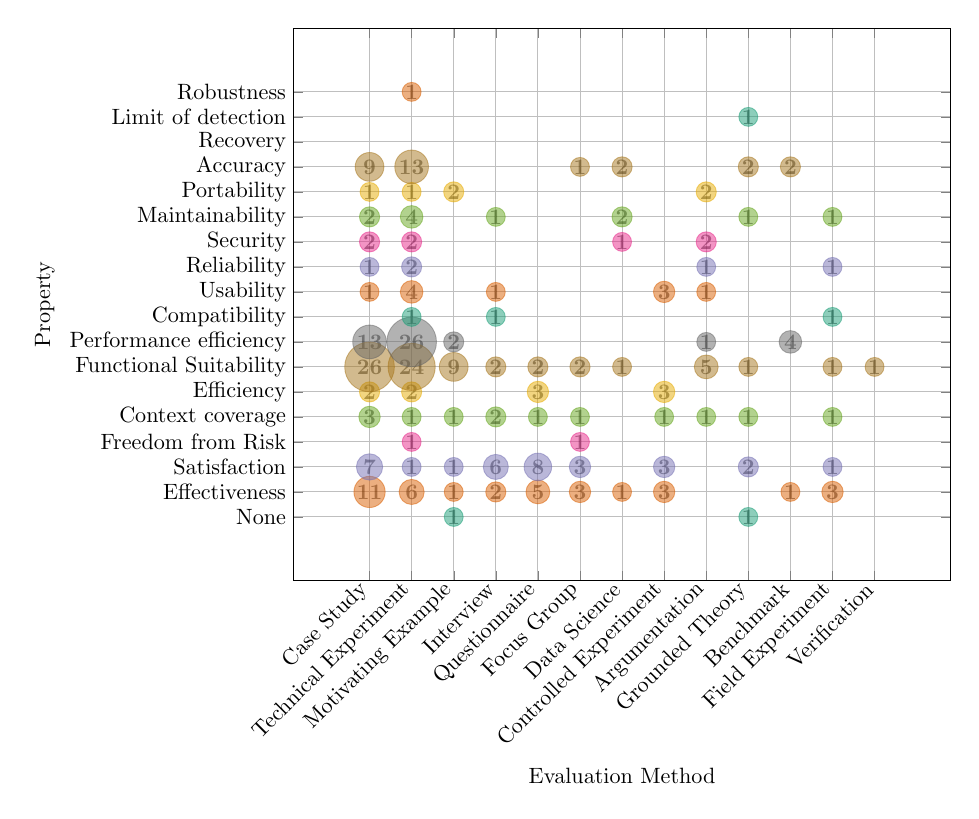
\begin{tikzpicture}[scale=.8]
\pgfplotsset{cycle list/Dark2}
\begin{axis}[width=.99\linewidth,
    enlargelimits=0.15,
    x tick label style={rotate=45,anchor=east},
    xtick={0,1,2,3,4,5,6,7,8,9,10,11,12}, xticklabels={Case Study,Technical Experiment,Motivating Example,Interview,Questionnaire,Focus Group,Data Science,Controlled Experiment,Argumentation,Grounded Theory,Benchmark,Field Experiment,Verification},
    xlabel={Evaluation Method},
    ytick={0,1,2,3,4,5,6,7,8,9,10,11,12,13,14,15,16,17}, yticklabels={None,Effectiveness,Satisfaction,Freedom from Risk,Context coverage,Efficiency,Functional Suitability,Performance efficiency,Compatibility,Usability,Reliability,Security,Maintainability,Portability,Accuracy,Recovery,Limit of detection,Robustness},
    ylabel={Property},
    grid=both,
    scatter,scatter src=y,
    scatter/classes={0={draw=Dark2-A,fill=Dark2-A}, 1={draw=Dark2-B,fill=Dark2-B}, 2={draw=Dark2-C,fill=Dark2-C}, 3={draw=Dark2-D,fill=Dark2-D}, 4={draw=Dark2-E,fill=Dark2-E}, 5={draw=Dark2-F,fill=Dark2-F}, 6={draw=Dark2-G,fill=Dark2-G}, 7={draw=Dark2-H,fill=Dark2-H}, 8={draw=Dark2-A,fill=Dark2-A}, 9={draw=Dark2-B,fill=Dark2-B}, 10={draw=Dark2-C,fill=Dark2-C}, 11={draw=Dark2-D,fill=Dark2-D}, 12={draw=Dark2-E,fill=Dark2-E}, 13={draw=Dark2-F,fill=Dark2-F}, 14={draw=Dark2-G,fill=Dark2-G}, 15={draw=Dark2-H,fill=Dark2-H}, 16={draw=Dark2-A,fill=Dark2-A}, 17={draw=Dark2-B,fill=Dark2-B}}
]

\addplot+[mark=*,mark size=7.056,opacity=0.5,text=black] coordinates { (0,1) } node[text=black,font=\bfseries] {11};
\addplot+[mark=*,mark size=5.944,opacity=0.5,text=black] coordinates { (0,2) } node[text=black,font=\bfseries] {7};
\addplot+[mark=*,mark size=4.833,opacity=0.5,text=black] coordinates { (0,4) } node[text=black,font=\bfseries] {3};
\addplot+[mark=*,mark size=4.556,opacity=0.5,text=black] coordinates { (0,5) } node[text=black,font=\bfseries] {2};
\addplot+[mark=*,mark size=11.222,opacity=0.5,text=black] coordinates { (0,6) } node[text=black,font=\bfseries] {26};
\addplot+[mark=*,mark size=7.611,opacity=0.5,text=black] coordinates { (0,7) } node[text=black,font=\bfseries] {13};
\addplot+[mark=*,mark size=4.278,opacity=0.5,text=black] coordinates { (0,9) } node[text=black,font=\bfseries] {1};
\addplot+[mark=*,mark size=4.278,opacity=0.5,text=black] coordinates { (0,10) } node[text=black,font=\bfseries] {1};
\addplot+[mark=*,mark size=4.556,opacity=0.5,text=black] coordinates { (0,11) } node[text=black,font=\bfseries] {2};
\addplot+[mark=*,mark size=4.556,opacity=0.5,text=black] coordinates { (0,12) } node[text=black,font=\bfseries] {2};
\addplot+[mark=*,mark size=4.278,opacity=0.5,text=black] coordinates { (0,13) } node[text=black,font=\bfseries] {1};
\addplot+[mark=*,mark size=6.500,opacity=0.5,text=black] coordinates { (0,14) } node[text=black,font=\bfseries] {9};
\addplot+[mark=*,mark size=5.667,opacity=0.5,text=black] coordinates { (1,1) } node[text=black,font=\bfseries] {6};
\addplot+[mark=*,mark size=4.278,opacity=0.5,text=black] coordinates { (1,2) } node[text=black,font=\bfseries] {1};
\addplot+[mark=*,mark size=4.278,opacity=0.5,text=black] coordinates { (1,3) } node[text=black,font=\bfseries] {1};
\addplot+[mark=*,mark size=4.278,opacity=0.5,text=black] coordinates { (1,4) } node[text=black,font=\bfseries] {1};
\addplot+[mark=*,mark size=4.556,opacity=0.5,text=black] coordinates { (1,5) } node[text=black,font=\bfseries] {2};
\addplot+[mark=*,mark size=10.667,opacity=0.5,text=black] coordinates { (1,6) } node[text=black,font=\bfseries] {24};
\addplot+[mark=*,mark size=11.222,opacity=0.5,text=black] coordinates { (1,7) } node[text=black,font=\bfseries] {26};
\addplot+[mark=*,mark size=4.278,opacity=0.5,text=black] coordinates { (1,8) } node[text=black,font=\bfseries] {1};
\addplot+[mark=*,mark size=5.111,opacity=0.5,text=black] coordinates { (1,9) } node[text=black,font=\bfseries] {4};
\addplot+[mark=*,mark size=4.556,opacity=0.5,text=black] coordinates { (1,10) } node[text=black,font=\bfseries] {2};
\addplot+[mark=*,mark size=4.556,opacity=0.5,text=black] coordinates { (1,11) } node[text=black,font=\bfseries] {2};
\addplot+[mark=*,mark size=5.111,opacity=0.5,text=black] coordinates { (1,12) } node[text=black,font=\bfseries] {4};
\addplot+[mark=*,mark size=4.278,opacity=0.5,text=black] coordinates { (1,13) } node[text=black,font=\bfseries] {1};
\addplot+[mark=*,mark size=7.611,opacity=0.5,text=black] coordinates { (1,14) } node[text=black,font=\bfseries] {13};
\addplot+[mark=*,mark size=4.278,opacity=0.5,text=black] coordinates { (1,17) } node[text=black,font=\bfseries] {1};
\addplot+[mark=*,mark size=4.278,opacity=0.5,text=black] coordinates { (2,0) } node[text=black,font=\bfseries] {1};
\addplot+[mark=*,mark size=4.278,opacity=0.5,text=black] coordinates { (2,1) } node[text=black,font=\bfseries] {1};
\addplot+[mark=*,mark size=4.278,opacity=0.5,text=black] coordinates { (2,2) } node[text=black,font=\bfseries] {1};
\addplot+[mark=*,mark size=4.278,opacity=0.5,text=black] coordinates { (2,4) } node[text=black,font=\bfseries] {1};
\addplot+[mark=*,mark size=6.500,opacity=0.5,text=black] coordinates { (2,6) } node[text=black,font=\bfseries] {9};
\addplot+[mark=*,mark size=4.556,opacity=0.5,text=black] coordinates { (2,7) } node[text=black,font=\bfseries] {2};
\addplot+[mark=*,mark size=4.556,opacity=0.5,text=black] coordinates { (2,13) } node[text=black,font=\bfseries] {2};
\addplot+[mark=*,mark size=4.556,opacity=0.5,text=black] coordinates { (3,1) } node[text=black,font=\bfseries] {2};
\addplot+[mark=*,mark size=5.667,opacity=0.5,text=black] coordinates { (3,2) } node[text=black,font=\bfseries] {6};
\addplot+[mark=*,mark size=4.556,opacity=0.5,text=black] coordinates { (3,4) } node[text=black,font=\bfseries] {2};
\addplot+[mark=*,mark size=4.556,opacity=0.5,text=black] coordinates { (3,6) } node[text=black,font=\bfseries] {2};
\addplot+[mark=*,mark size=4.278,opacity=0.5,text=black] coordinates { (3,8) } node[text=black,font=\bfseries] {1};
\addplot+[mark=*,mark size=4.278,opacity=0.5,text=black] coordinates { (3,9) } node[text=black,font=\bfseries] {1};
\addplot+[mark=*,mark size=4.278,opacity=0.5,text=black] coordinates { (3,12) } node[text=black,font=\bfseries] {1};
\addplot+[mark=*,mark size=5.389,opacity=0.5,text=black] coordinates { (4,1) } node[text=black,font=\bfseries] {5};
\addplot+[mark=*,mark size=6.222,opacity=0.5,text=black] coordinates { (4,2) } node[text=black,font=\bfseries] {8};
\addplot+[mark=*,mark size=4.278,opacity=0.5,text=black] coordinates { (4,4) } node[text=black,font=\bfseries] {1};
\addplot+[mark=*,mark size=4.833,opacity=0.5,text=black] coordinates { (4,5) } node[text=black,font=\bfseries] {3};
\addplot+[mark=*,mark size=4.556,opacity=0.5,text=black] coordinates { (4,6) } node[text=black,font=\bfseries] {2};
\addplot+[mark=*,mark size=4.833,opacity=0.5,text=black] coordinates { (5,1) } node[text=black,font=\bfseries] {3};
\addplot+[mark=*,mark size=4.833,opacity=0.5,text=black] coordinates { (5,2) } node[text=black,font=\bfseries] {3};
\addplot+[mark=*,mark size=4.278,opacity=0.5,text=black] coordinates { (5,3) } node[text=black,font=\bfseries] {1};
\addplot+[mark=*,mark size=4.278,opacity=0.5,text=black] coordinates { (5,4) } node[text=black,font=\bfseries] {1};
\addplot+[mark=*,mark size=4.556,opacity=0.5,text=black] coordinates { (5,6) } node[text=black,font=\bfseries] {2};
\addplot+[mark=*,mark size=4.278,opacity=0.5,text=black] coordinates { (5,14) } node[text=black,font=\bfseries] {1};
\addplot+[mark=*,mark size=4.278,opacity=0.5,text=black] coordinates { (6,1) } node[text=black,font=\bfseries] {1};
\addplot+[mark=*,mark size=4.278,opacity=0.5,text=black] coordinates { (6,6) } node[text=black,font=\bfseries] {1};
\addplot+[mark=*,mark size=4.278,opacity=0.5,text=black] coordinates { (6,11) } node[text=black,font=\bfseries] {1};
\addplot+[mark=*,mark size=4.556,opacity=0.5,text=black] coordinates { (6,12) } node[text=black,font=\bfseries] {2};
\addplot+[mark=*,mark size=4.556,opacity=0.5,text=black] coordinates { (6,14) } node[text=black,font=\bfseries] {2};
\addplot+[mark=*,mark size=4.833,opacity=0.5,text=black] coordinates { (7,1) } node[text=black,font=\bfseries] {3};
\addplot+[mark=*,mark size=4.833,opacity=0.5,text=black] coordinates { (7,2) } node[text=black,font=\bfseries] {3};
\addplot+[mark=*,mark size=4.278,opacity=0.5,text=black] coordinates { (7,4) } node[text=black,font=\bfseries] {1};
\addplot+[mark=*,mark size=4.833,opacity=0.5,text=black] coordinates { (7,5) } node[text=black,font=\bfseries] {3};
\addplot+[mark=*,mark size=4.833,opacity=0.5,text=black] coordinates { (7,9) } node[text=black,font=\bfseries] {3};
\addplot+[mark=*,mark size=4.278,opacity=0.5,text=black] coordinates { (8,4) } node[text=black,font=\bfseries] {1};
\addplot+[mark=*,mark size=5.389,opacity=0.5,text=black] coordinates { (8,6) } node[text=black,font=\bfseries] {5};
\addplot+[mark=*,mark size=4.278,opacity=0.5,text=black] coordinates { (8,7) } node[text=black,font=\bfseries] {1};
\addplot+[mark=*,mark size=4.278,opacity=0.5,text=black] coordinates { (8,9) } node[text=black,font=\bfseries] {1};
\addplot+[mark=*,mark size=4.278,opacity=0.5,text=black] coordinates { (8,10) } node[text=black,font=\bfseries] {1};
\addplot+[mark=*,mark size=4.556,opacity=0.5,text=black] coordinates { (8,11) } node[text=black,font=\bfseries] {2};
\addplot+[mark=*,mark size=4.556,opacity=0.5,text=black] coordinates { (8,13) } node[text=black,font=\bfseries] {2};
\addplot+[mark=*,mark size=4.278,opacity=0.5,text=black] coordinates { (9,0) } node[text=black,font=\bfseries] {1};
\addplot+[mark=*,mark size=4.556,opacity=0.5,text=black] coordinates { (9,2) } node[text=black,font=\bfseries] {2};
\addplot+[mark=*,mark size=4.278,opacity=0.5,text=black] coordinates { (9,4) } node[text=black,font=\bfseries] {1};
\addplot+[mark=*,mark size=4.278,opacity=0.5,text=black] coordinates { (9,6) } node[text=black,font=\bfseries] {1};
\addplot+[mark=*,mark size=4.278,opacity=0.5,text=black] coordinates { (9,12) } node[text=black,font=\bfseries] {1};
\addplot+[mark=*,mark size=4.556,opacity=0.5,text=black] coordinates { (9,14) } node[text=black,font=\bfseries] {2};
\addplot+[mark=*,mark size=4.278,opacity=0.5,text=black] coordinates { (9,16) } node[text=black,font=\bfseries] {1};
\addplot+[mark=*,mark size=4.278,opacity=0.5,text=black] coordinates { (10,1) } node[text=black,font=\bfseries] {1};
\addplot+[mark=*,mark size=5.111,opacity=0.5,text=black] coordinates { (10,7) } node[text=black,font=\bfseries] {4};
\addplot+[mark=*,mark size=4.556,opacity=0.5,text=black] coordinates { (10,14) } node[text=black,font=\bfseries] {2};
\addplot+[mark=*,mark size=4.833,opacity=0.5,text=black] coordinates { (11,1) } node[text=black,font=\bfseries] {3};
\addplot+[mark=*,mark size=4.278,opacity=0.5,text=black] coordinates { (11,2) } node[text=black,font=\bfseries] {1};
\addplot+[mark=*,mark size=4.278,opacity=0.5,text=black] coordinates { (11,4) } node[text=black,font=\bfseries] {1};
\addplot+[mark=*,mark size=4.278,opacity=0.5,text=black] coordinates { (11,6) } node[text=black,font=\bfseries] {1};
\addplot+[mark=*,mark size=4.278,opacity=0.5,text=black] coordinates { (11,8) } node[text=black,font=\bfseries] {1};
\addplot+[mark=*,mark size=4.278,opacity=0.5,text=black] coordinates { (11,10) } node[text=black,font=\bfseries] {1};
\addplot+[mark=*,mark size=4.278,opacity=0.5,text=black] coordinates { (11,12) } node[text=black,font=\bfseries] {1};
\addplot+[mark=*,mark size=4.278,opacity=0.5,text=black] coordinates { (12,6) } node[text=black,font=\bfseries] {1};


\end{axis}
\end{tikzpicture}
\end{center}
%\caption{Portfolio f\"ur Evaluation Method und Property (Gr\"o\ss{}e entspricht der Anzahl)}\label{fig:port_evaluationmethod_property}
%\end{figure}



\section{Evaluation Method vs. Paper Class}

%\subsection{Portfolio f\"ur Paper Class und Evaluation Method (Gr\"o\ss{}e entspricht der Anzahl)}
%\begin{figure}
\begin{center}
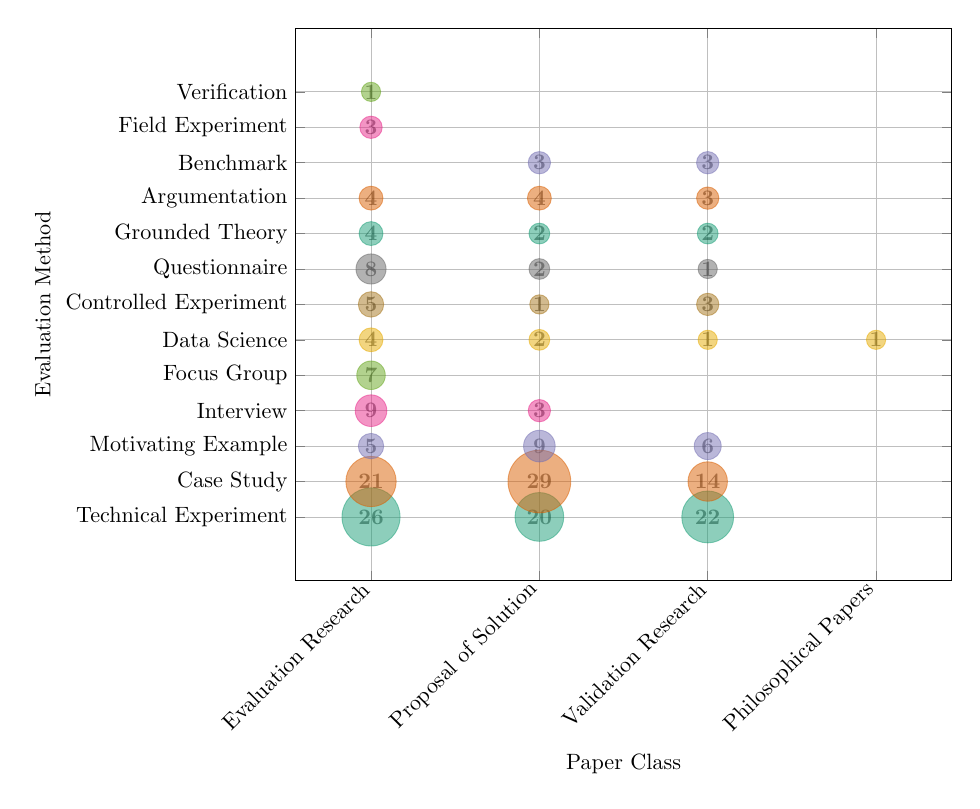
\begin{tikzpicture}[scale=.8]
\pgfplotsset{cycle list/Dark2}
\begin{axis}[width=.99\linewidth,
    enlargelimits=0.15,
    x tick label style={rotate=45,anchor=east},
    xtick={0,1,2,3}, xticklabels={Evaluation Research,Proposal of Solution,Validation Research,Philosophical Papers},
    xlabel={Paper Class},
    ytick={0,1,2,3,4,5,6,7,8,9,10,11,12}, yticklabels={Technical Experiment,Case Study,Motivating Example,Interview,Focus Group,Data Science,Controlled Experiment,Questionnaire,Grounded Theory,Argumentation,Benchmark,Field Experiment,Verification},
    ylabel={Evaluation Method},
    grid=both,
    scatter,scatter src=y,
    scatter/classes={0={draw=Dark2-A,fill=Dark2-A}, 1={draw=Dark2-B,fill=Dark2-B}, 2={draw=Dark2-C,fill=Dark2-C}, 3={draw=Dark2-D,fill=Dark2-D}, 4={draw=Dark2-E,fill=Dark2-E}, 5={draw=Dark2-F,fill=Dark2-F}, 6={draw=Dark2-G,fill=Dark2-G}, 7={draw=Dark2-H,fill=Dark2-H}, 8={draw=Dark2-A,fill=Dark2-A}, 9={draw=Dark2-B,fill=Dark2-B}, 10={draw=Dark2-C,fill=Dark2-C}, 11={draw=Dark2-D,fill=Dark2-D}, 12={draw=Dark2-E,fill=Dark2-E}}
]

\addplot+[mark=*,mark size=13.123,opacity=0.5,text=black] coordinates { (0,0) } node[text=black,font=\bfseries] {26};
\addplot+[mark=*,mark size=11.368,opacity=0.5,text=black] coordinates { (0,1) } node[text=black,font=\bfseries] {21};
\addplot+[mark=*,mark size=5.754,opacity=0.5,text=black] coordinates { (0,2) } node[text=black,font=\bfseries] {5};
\addplot+[mark=*,mark size=7.158,opacity=0.5,text=black] coordinates { (0,3) } node[text=black,font=\bfseries] {9};
\addplot+[mark=*,mark size=6.456,opacity=0.5,text=black] coordinates { (0,4) } node[text=black,font=\bfseries] {7};
\addplot+[mark=*,mark size=5.404,opacity=0.5,text=black] coordinates { (0,5) } node[text=black,font=\bfseries] {4};
\addplot+[mark=*,mark size=5.754,opacity=0.5,text=black] coordinates { (0,6) } node[text=black,font=\bfseries] {5};
\addplot+[mark=*,mark size=6.807,opacity=0.5,text=black] coordinates { (0,7) } node[text=black,font=\bfseries] {8};
\addplot+[mark=*,mark size=5.404,opacity=0.5,text=black] coordinates { (0,8) } node[text=black,font=\bfseries] {4};
\addplot+[mark=*,mark size=5.404,opacity=0.5,text=black] coordinates { (0,9) } node[text=black,font=\bfseries] {4};
\addplot+[mark=*,mark size=5.053,opacity=0.5,text=black] coordinates { (0,11) } node[text=black,font=\bfseries] {3};
\addplot+[mark=*,mark size=4.351,opacity=0.5,text=black] coordinates { (0,12) } node[text=black,font=\bfseries] {1};
\addplot+[mark=*,mark size=11.018,opacity=0.5,text=black] coordinates { (1,0) } node[text=black,font=\bfseries] {20};
\addplot+[mark=*,mark size=14.175,opacity=0.5,text=black] coordinates { (1,1) } node[text=black,font=\bfseries] {29};
\addplot+[mark=*,mark size=7.158,opacity=0.5,text=black] coordinates { (1,2) } node[text=black,font=\bfseries] {9};
\addplot+[mark=*,mark size=5.053,opacity=0.5,text=black] coordinates { (1,3) } node[text=black,font=\bfseries] {3};
\addplot+[mark=*,mark size=4.702,opacity=0.5,text=black] coordinates { (1,5) } node[text=black,font=\bfseries] {2};
\addplot+[mark=*,mark size=4.351,opacity=0.5,text=black] coordinates { (1,6) } node[text=black,font=\bfseries] {1};
\addplot+[mark=*,mark size=4.702,opacity=0.5,text=black] coordinates { (1,7) } node[text=black,font=\bfseries] {2};
\addplot+[mark=*,mark size=4.702,opacity=0.5,text=black] coordinates { (1,8) } node[text=black,font=\bfseries] {2};
\addplot+[mark=*,mark size=5.404,opacity=0.5,text=black] coordinates { (1,9) } node[text=black,font=\bfseries] {4};
\addplot+[mark=*,mark size=5.053,opacity=0.5,text=black] coordinates { (1,10) } node[text=black,font=\bfseries] {3};
\addplot+[mark=*,mark size=11.719,opacity=0.5,text=black] coordinates { (2,0) } node[text=black,font=\bfseries] {22};
\addplot+[mark=*,mark size=8.912,opacity=0.5,text=black] coordinates { (2,1) } node[text=black,font=\bfseries] {14};
\addplot+[mark=*,mark size=6.105,opacity=0.5,text=black] coordinates { (2,2) } node[text=black,font=\bfseries] {6};
\addplot+[mark=*,mark size=4.351,opacity=0.5,text=black] coordinates { (2,5) } node[text=black,font=\bfseries] {1};
\addplot+[mark=*,mark size=5.053,opacity=0.5,text=black] coordinates { (2,6) } node[text=black,font=\bfseries] {3};
\addplot+[mark=*,mark size=4.351,opacity=0.5,text=black] coordinates { (2,7) } node[text=black,font=\bfseries] {1};
\addplot+[mark=*,mark size=4.702,opacity=0.5,text=black] coordinates { (2,8) } node[text=black,font=\bfseries] {2};
\addplot+[mark=*,mark size=5.053,opacity=0.5,text=black] coordinates { (2,9) } node[text=black,font=\bfseries] {3};
\addplot+[mark=*,mark size=5.053,opacity=0.5,text=black] coordinates { (2,10) } node[text=black,font=\bfseries] {3};
\addplot+[mark=*,mark size=4.351,opacity=0.5,text=black] coordinates { (3,5) } node[text=black,font=\bfseries] {1};


\end{axis}
\end{tikzpicture}
\end{center}
%\caption{Portfolio f\"ur Paper Class und Evaluation Method (Gr\"o\ss{}e entspricht der Anzahl)}\label{fig:port_paperclass_evaluationmethod}
%\end{figure}


%\subsection{Portfolio f\"ur Evaluation Method und Paper Class (Gr\"o\ss{}e entspricht der Anzahl)}
%\begin{figure}
\begin{center}
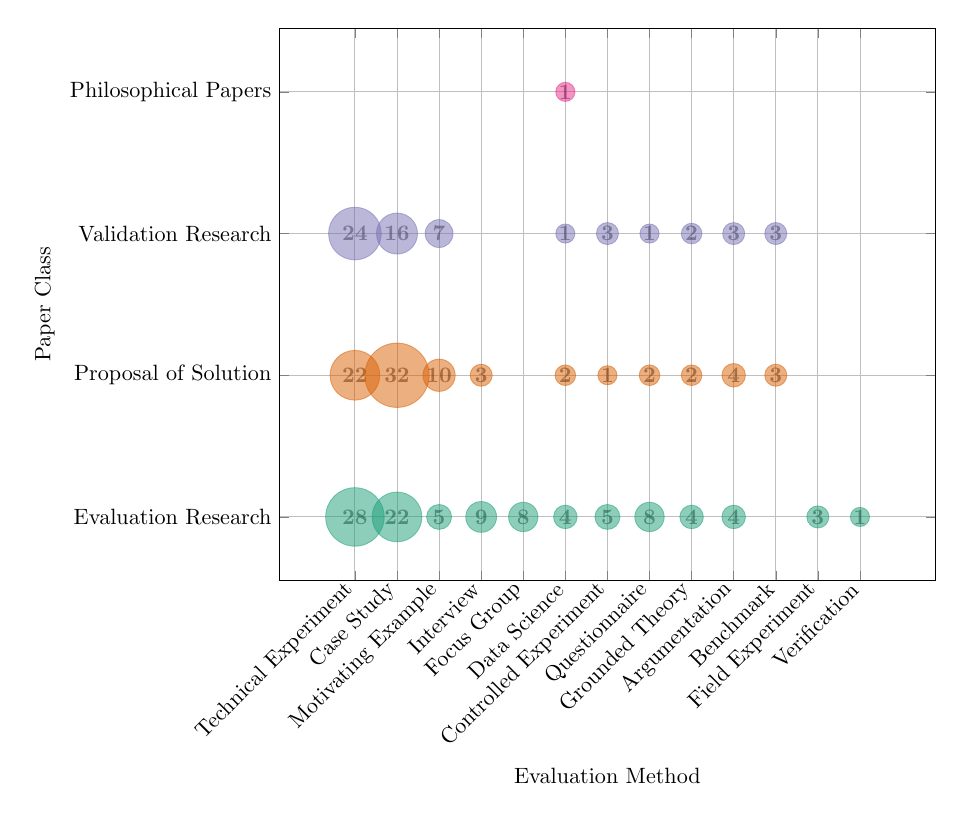
\begin{tikzpicture}[scale=.8]
\pgfplotsset{cycle list/Dark2}
\begin{axis}[width=.99\linewidth,
    enlargelimits=0.15,
    x tick label style={rotate=45,anchor=east},
    xtick={0,1,2,3,4,5,6,7,8,9,10,11,12}, xticklabels={Technical Experiment,Case Study,Motivating Example,Interview,Focus Group,Data Science,Controlled Experiment,Questionnaire,Grounded Theory,Argumentation,Benchmark,Field Experiment,Verification},
    xlabel={Evaluation Method},
    ytick={0,1,2,3}, yticklabels={Evaluation Research,Proposal of Solution,Validation Research,Philosophical Papers},
    ylabel={Paper Class},
    grid=both,
    scatter,scatter src=y,
    scatter/classes={0={draw=Dark2-A,fill=Dark2-A}, 1={draw=Dark2-B,fill=Dark2-B}, 2={draw=Dark2-C,fill=Dark2-C}, 3={draw=Dark2-D,fill=Dark2-D}}
]

\addplot+[mark=*,mark size=13.218,opacity=0.5,text=black] coordinates { (0,0) } node[text=black,font=\bfseries] {28};
\addplot+[mark=*,mark size=11.243,opacity=0.5,text=black] coordinates { (0,1) } node[text=black,font=\bfseries] {22};
\addplot+[mark=*,mark size=11.901,opacity=0.5,text=black] coordinates { (0,2) } node[text=black,font=\bfseries] {24};
\addplot+[mark=*,mark size=11.243,opacity=0.5,text=black] coordinates { (1,0) } node[text=black,font=\bfseries] {22};
\addplot+[mark=*,mark size=14.535,opacity=0.5,text=black] coordinates { (1,1) } node[text=black,font=\bfseries] {32};
\addplot+[mark=*,mark size=9.267,opacity=0.5,text=black] coordinates { (1,2) } node[text=black,font=\bfseries] {16};
\addplot+[mark=*,mark size=5.646,opacity=0.5,text=black] coordinates { (2,0) } node[text=black,font=\bfseries] {5};
\addplot+[mark=*,mark size=7.292,opacity=0.5,text=black] coordinates { (2,1) } node[text=black,font=\bfseries] {10};
\addplot+[mark=*,mark size=6.305,opacity=0.5,text=black] coordinates { (2,2) } node[text=black,font=\bfseries] {7};
\addplot+[mark=*,mark size=6.963,opacity=0.5,text=black] coordinates { (3,0) } node[text=black,font=\bfseries] {9};
\addplot+[mark=*,mark size=4.988,opacity=0.5,text=black] coordinates { (3,1) } node[text=black,font=\bfseries] {3};
\addplot+[mark=*,mark size=6.634,opacity=0.5,text=black] coordinates { (4,0) } node[text=black,font=\bfseries] {8};
\addplot+[mark=*,mark size=5.317,opacity=0.5,text=black] coordinates { (5,0) } node[text=black,font=\bfseries] {4};
\addplot+[mark=*,mark size=4.658,opacity=0.5,text=black] coordinates { (5,1) } node[text=black,font=\bfseries] {2};
\addplot+[mark=*,mark size=4.329,opacity=0.5,text=black] coordinates { (5,2) } node[text=black,font=\bfseries] {1};
\addplot+[mark=*,mark size=4.329,opacity=0.5,text=black] coordinates { (5,3) } node[text=black,font=\bfseries] {1};
\addplot+[mark=*,mark size=5.646,opacity=0.5,text=black] coordinates { (6,0) } node[text=black,font=\bfseries] {5};
\addplot+[mark=*,mark size=4.329,opacity=0.5,text=black] coordinates { (6,1) } node[text=black,font=\bfseries] {1};
\addplot+[mark=*,mark size=4.988,opacity=0.5,text=black] coordinates { (6,2) } node[text=black,font=\bfseries] {3};
\addplot+[mark=*,mark size=6.634,opacity=0.5,text=black] coordinates { (7,0) } node[text=black,font=\bfseries] {8};
\addplot+[mark=*,mark size=4.658,opacity=0.5,text=black] coordinates { (7,1) } node[text=black,font=\bfseries] {2};
\addplot+[mark=*,mark size=4.329,opacity=0.5,text=black] coordinates { (7,2) } node[text=black,font=\bfseries] {1};
\addplot+[mark=*,mark size=5.317,opacity=0.5,text=black] coordinates { (8,0) } node[text=black,font=\bfseries] {4};
\addplot+[mark=*,mark size=4.658,opacity=0.5,text=black] coordinates { (8,1) } node[text=black,font=\bfseries] {2};
\addplot+[mark=*,mark size=4.658,opacity=0.5,text=black] coordinates { (8,2) } node[text=black,font=\bfseries] {2};
\addplot+[mark=*,mark size=5.317,opacity=0.5,text=black] coordinates { (9,0) } node[text=black,font=\bfseries] {4};
\addplot+[mark=*,mark size=5.317,opacity=0.5,text=black] coordinates { (9,1) } node[text=black,font=\bfseries] {4};
\addplot+[mark=*,mark size=4.988,opacity=0.5,text=black] coordinates { (9,2) } node[text=black,font=\bfseries] {3};
\addplot+[mark=*,mark size=4.988,opacity=0.5,text=black] coordinates { (10,1) } node[text=black,font=\bfseries] {3};
\addplot+[mark=*,mark size=4.988,opacity=0.5,text=black] coordinates { (10,2) } node[text=black,font=\bfseries] {3};
\addplot+[mark=*,mark size=4.988,opacity=0.5,text=black] coordinates { (11,0) } node[text=black,font=\bfseries] {3};
\addplot+[mark=*,mark size=4.329,opacity=0.5,text=black] coordinates { (12,0) } node[text=black,font=\bfseries] {1};


\end{axis}
\end{tikzpicture}
\end{center}
%\caption{Portfolio f\"ur Evaluation Method und Paper Class (Gr\"o\ss{}e entspricht der Anzahl)}\label{fig:port_evaluationmethod_paperclass}
%\end{figure}



\section{Evaluation Method vs Threats to Validity}

%\subsection{Portfolio f\"ur Evaluation Method und Threats To Validity (Gr\"o\ss{}e entspricht der Anzahl)}
%\begin{figure}
\begin{center}
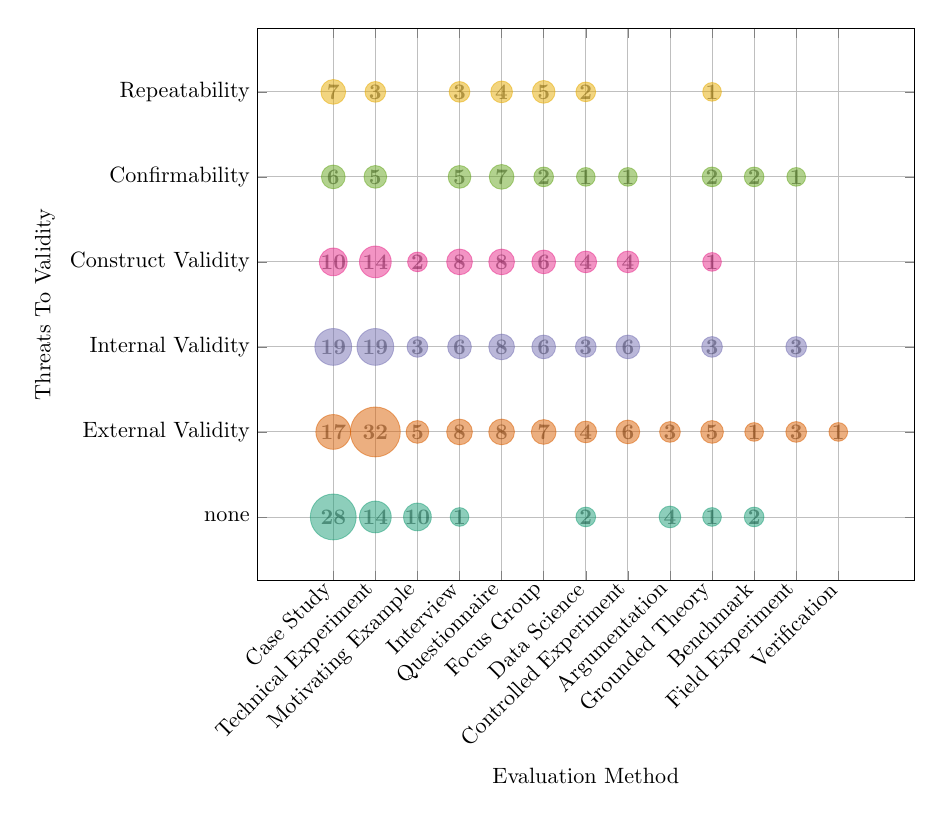
\begin{tikzpicture}[scale=.8]
\pgfplotsset{cycle list/Dark2}
\begin{axis}[width=.99\linewidth,
    enlargelimits=0.15,
    x tick label style={rotate=45,anchor=east},
    xtick={0,1,2,3,4,5,6,7,8,9,10,11,12}, xticklabels={Case Study,Technical Experiment,Motivating Example,Interview,Questionnaire,Focus Group,Data Science,Controlled Experiment,Argumentation,Grounded Theory,Benchmark,Field Experiment,Verification},
    xlabel={Evaluation Method},
    ytick={0,1,2,3,4,5}, yticklabels={none,External Validity,Internal Validity,Construct Validity,Confirmability,Repeatability},
    ylabel={Threats To Validity},
    grid=both,
    scatter,scatter src=y,
    scatter/classes={0={draw=Dark2-A,fill=Dark2-A}, 1={draw=Dark2-B,fill=Dark2-B}, 2={draw=Dark2-C,fill=Dark2-C}, 3={draw=Dark2-D,fill=Dark2-D}, 4={draw=Dark2-E,fill=Dark2-E}, 5={draw=Dark2-F,fill=Dark2-F}}
]

\addplot+[mark=*,mark size=10.364,opacity=0.5,text=black] coordinates { (0,0) } node[text=black,font=\bfseries] {28};
\addplot+[mark=*,mark size=7.864,opacity=0.5,text=black] coordinates { (0,1) } node[text=black,font=\bfseries] {17};
\addplot+[mark=*,mark size=8.318,opacity=0.5,text=black] coordinates { (0,2) } node[text=black,font=\bfseries] {19};
\addplot+[mark=*,mark size=6.273,opacity=0.5,text=black] coordinates { (0,3) } node[text=black,font=\bfseries] {10};
\addplot+[mark=*,mark size=5.364,opacity=0.5,text=black] coordinates { (0,4) } node[text=black,font=\bfseries] {6};
\addplot+[mark=*,mark size=5.591,opacity=0.5,text=black] coordinates { (0,5) } node[text=black,font=\bfseries] {7};
\addplot+[mark=*,mark size=7.182,opacity=0.5,text=black] coordinates { (1,0) } node[text=black,font=\bfseries] {14};
\addplot+[mark=*,mark size=11.273,opacity=0.5,text=black] coordinates { (1,1) } node[text=black,font=\bfseries] {32};
\addplot+[mark=*,mark size=8.318,opacity=0.5,text=black] coordinates { (1,2) } node[text=black,font=\bfseries] {19};
\addplot+[mark=*,mark size=7.182,opacity=0.5,text=black] coordinates { (1,3) } node[text=black,font=\bfseries] {14};
\addplot+[mark=*,mark size=5.136,opacity=0.5,text=black] coordinates { (1,4) } node[text=black,font=\bfseries] {5};
\addplot+[mark=*,mark size=4.682,opacity=0.5,text=black] coordinates { (1,5) } node[text=black,font=\bfseries] {3};
\addplot+[mark=*,mark size=6.273,opacity=0.5,text=black] coordinates { (2,0) } node[text=black,font=\bfseries] {10};
\addplot+[mark=*,mark size=5.136,opacity=0.5,text=black] coordinates { (2,1) } node[text=black,font=\bfseries] {5};
\addplot+[mark=*,mark size=4.682,opacity=0.5,text=black] coordinates { (2,2) } node[text=black,font=\bfseries] {3};
\addplot+[mark=*,mark size=4.455,opacity=0.5,text=black] coordinates { (2,3) } node[text=black,font=\bfseries] {2};
\addplot+[mark=*,mark size=4.227,opacity=0.5,text=black] coordinates { (3,0) } node[text=black,font=\bfseries] {1};
\addplot+[mark=*,mark size=5.818,opacity=0.5,text=black] coordinates { (3,1) } node[text=black,font=\bfseries] {8};
\addplot+[mark=*,mark size=5.364,opacity=0.5,text=black] coordinates { (3,2) } node[text=black,font=\bfseries] {6};
\addplot+[mark=*,mark size=5.818,opacity=0.5,text=black] coordinates { (3,3) } node[text=black,font=\bfseries] {8};
\addplot+[mark=*,mark size=5.136,opacity=0.5,text=black] coordinates { (3,4) } node[text=black,font=\bfseries] {5};
\addplot+[mark=*,mark size=4.682,opacity=0.5,text=black] coordinates { (3,5) } node[text=black,font=\bfseries] {3};
\addplot+[mark=*,mark size=5.818,opacity=0.5,text=black] coordinates { (4,1) } node[text=black,font=\bfseries] {8};
\addplot+[mark=*,mark size=5.818,opacity=0.5,text=black] coordinates { (4,2) } node[text=black,font=\bfseries] {8};
\addplot+[mark=*,mark size=5.818,opacity=0.5,text=black] coordinates { (4,3) } node[text=black,font=\bfseries] {8};
\addplot+[mark=*,mark size=5.591,opacity=0.5,text=black] coordinates { (4,4) } node[text=black,font=\bfseries] {7};
\addplot+[mark=*,mark size=4.909,opacity=0.5,text=black] coordinates { (4,5) } node[text=black,font=\bfseries] {4};
\addplot+[mark=*,mark size=5.591,opacity=0.5,text=black] coordinates { (5,1) } node[text=black,font=\bfseries] {7};
\addplot+[mark=*,mark size=5.364,opacity=0.5,text=black] coordinates { (5,2) } node[text=black,font=\bfseries] {6};
\addplot+[mark=*,mark size=5.364,opacity=0.5,text=black] coordinates { (5,3) } node[text=black,font=\bfseries] {6};
\addplot+[mark=*,mark size=4.455,opacity=0.5,text=black] coordinates { (5,4) } node[text=black,font=\bfseries] {2};
\addplot+[mark=*,mark size=5.136,opacity=0.5,text=black] coordinates { (5,5) } node[text=black,font=\bfseries] {5};
\addplot+[mark=*,mark size=4.455,opacity=0.5,text=black] coordinates { (6,0) } node[text=black,font=\bfseries] {2};
\addplot+[mark=*,mark size=4.909,opacity=0.5,text=black] coordinates { (6,1) } node[text=black,font=\bfseries] {4};
\addplot+[mark=*,mark size=4.682,opacity=0.5,text=black] coordinates { (6,2) } node[text=black,font=\bfseries] {3};
\addplot+[mark=*,mark size=4.909,opacity=0.5,text=black] coordinates { (6,3) } node[text=black,font=\bfseries] {4};
\addplot+[mark=*,mark size=4.227,opacity=0.5,text=black] coordinates { (6,4) } node[text=black,font=\bfseries] {1};
\addplot+[mark=*,mark size=4.455,opacity=0.5,text=black] coordinates { (6,5) } node[text=black,font=\bfseries] {2};
\addplot+[mark=*,mark size=5.364,opacity=0.5,text=black] coordinates { (7,1) } node[text=black,font=\bfseries] {6};
\addplot+[mark=*,mark size=5.364,opacity=0.5,text=black] coordinates { (7,2) } node[text=black,font=\bfseries] {6};
\addplot+[mark=*,mark size=4.909,opacity=0.5,text=black] coordinates { (7,3) } node[text=black,font=\bfseries] {4};
\addplot+[mark=*,mark size=4.227,opacity=0.5,text=black] coordinates { (7,4) } node[text=black,font=\bfseries] {1};
\addplot+[mark=*,mark size=4.909,opacity=0.5,text=black] coordinates { (8,0) } node[text=black,font=\bfseries] {4};
\addplot+[mark=*,mark size=4.682,opacity=0.5,text=black] coordinates { (8,1) } node[text=black,font=\bfseries] {3};
\addplot+[mark=*,mark size=4.227,opacity=0.5,text=black] coordinates { (9,0) } node[text=black,font=\bfseries] {1};
\addplot+[mark=*,mark size=5.136,opacity=0.5,text=black] coordinates { (9,1) } node[text=black,font=\bfseries] {5};
\addplot+[mark=*,mark size=4.682,opacity=0.5,text=black] coordinates { (9,2) } node[text=black,font=\bfseries] {3};
\addplot+[mark=*,mark size=4.227,opacity=0.5,text=black] coordinates { (9,3) } node[text=black,font=\bfseries] {1};
\addplot+[mark=*,mark size=4.455,opacity=0.5,text=black] coordinates { (9,4) } node[text=black,font=\bfseries] {2};
\addplot+[mark=*,mark size=4.227,opacity=0.5,text=black] coordinates { (9,5) } node[text=black,font=\bfseries] {1};
\addplot+[mark=*,mark size=4.455,opacity=0.5,text=black] coordinates { (10,0) } node[text=black,font=\bfseries] {2};
\addplot+[mark=*,mark size=4.227,opacity=0.5,text=black] coordinates { (10,1) } node[text=black,font=\bfseries] {1};
\addplot+[mark=*,mark size=4.455,opacity=0.5,text=black] coordinates { (10,4) } node[text=black,font=\bfseries] {2};
\addplot+[mark=*,mark size=4.682,opacity=0.5,text=black] coordinates { (11,1) } node[text=black,font=\bfseries] {3};
\addplot+[mark=*,mark size=4.682,opacity=0.5,text=black] coordinates { (11,2) } node[text=black,font=\bfseries] {3};
\addplot+[mark=*,mark size=4.227,opacity=0.5,text=black] coordinates { (11,4) } node[text=black,font=\bfseries] {1};
\addplot+[mark=*,mark size=4.227,opacity=0.5,text=black] coordinates { (12,1) } node[text=black,font=\bfseries] {1};


\end{axis}
\end{tikzpicture}
\end{center}
%\caption{Portfolio f\"ur Evaluation Method und Threats To Validity (Gr\"o\ss{}e entspricht der Anzahl)}\label{fig:port_evaluationmethod_threatstovalidity}
%\end{figure}


%\subsection{Portfolio f\"ur Threats To Validity und Evaluation Method (Gr\"o\ss{}e entspricht der Anzahl)}
%\begin{figure}
\begin{center}
\begin{tikzpicture}[scale=.8]
\pgfplotsset{cycle list/Dark2}
\begin{axis}[width=.99\linewidth,
    enlargelimits=0.15,
    x tick label style={rotate=45,anchor=east},
    xtick={0,1,2,3,4,5}, xticklabels={none,External Validity,Internal Validity,Construct Validity,Confirmability,Repeatability},
    xlabel={Threats To Validity},
    ytick={0,1,2,3,4,5,6,7,8,9,10,11,12}, yticklabels={Case Study,Technical Experiment,Motivating Example,Interview,Questionnaire,Focus Group,Data Science,Controlled Experiment,Argumentation,Grounded Theory,Benchmark,Field Experiment,Verification},
    ylabel={Evaluation Method},
    grid=both,
    scatter,scatter src=y,
    scatter/classes={0={draw=Dark2-A,fill=Dark2-A}, 1={draw=Dark2-B,fill=Dark2-B}, 2={draw=Dark2-C,fill=Dark2-C}, 3={draw=Dark2-D,fill=Dark2-D}, 4={draw=Dark2-E,fill=Dark2-E}, 5={draw=Dark2-F,fill=Dark2-F}, 6={draw=Dark2-G,fill=Dark2-G}, 7={draw=Dark2-H,fill=Dark2-H}, 8={draw=Dark2-A,fill=Dark2-A}, 9={draw=Dark2-B,fill=Dark2-B}, 10={draw=Dark2-C,fill=Dark2-C}, 11={draw=Dark2-D,fill=Dark2-D}, 12={draw=Dark2-E,fill=Dark2-E}}
]

\addplot+[mark=*,mark size=10.448,opacity=0.5,text=black] coordinates { (0,0) } node[text=black,font=\bfseries] {27};
\addplot+[mark=*,mark size=7.343,opacity=0.5,text=black] coordinates { (0,1) } node[text=black,font=\bfseries] {14};
\addplot+[mark=*,mark size=6.388,opacity=0.5,text=black] coordinates { (0,2) } node[text=black,font=\bfseries] {10};
\addplot+[mark=*,mark size=4.239,opacity=0.5,text=black] coordinates { (0,3) } node[text=black,font=\bfseries] {1};
\addplot+[mark=*,mark size=4.478,opacity=0.5,text=black] coordinates { (0,6) } node[text=black,font=\bfseries] {2};
\addplot+[mark=*,mark size=4.955,opacity=0.5,text=black] coordinates { (0,8) } node[text=black,font=\bfseries] {4};
\addplot+[mark=*,mark size=4.239,opacity=0.5,text=black] coordinates { (0,9) } node[text=black,font=\bfseries] {1};
\addplot+[mark=*,mark size=4.478,opacity=0.5,text=black] coordinates { (0,10) } node[text=black,font=\bfseries] {2};
\addplot+[mark=*,mark size=8.060,opacity=0.5,text=black] coordinates { (1,0) } node[text=black,font=\bfseries] {17};
\addplot+[mark=*,mark size=11.164,opacity=0.5,text=black] coordinates { (1,1) } node[text=black,font=\bfseries] {30};
\addplot+[mark=*,mark size=4.955,opacity=0.5,text=black] coordinates { (1,2) } node[text=black,font=\bfseries] {4};
\addplot+[mark=*,mark size=5.910,opacity=0.5,text=black] coordinates { (1,3) } node[text=black,font=\bfseries] {8};
\addplot+[mark=*,mark size=5.910,opacity=0.5,text=black] coordinates { (1,4) } node[text=black,font=\bfseries] {8};
\addplot+[mark=*,mark size=5.433,opacity=0.5,text=black] coordinates { (1,5) } node[text=black,font=\bfseries] {6};
\addplot+[mark=*,mark size=4.955,opacity=0.5,text=black] coordinates { (1,6) } node[text=black,font=\bfseries] {4};
\addplot+[mark=*,mark size=5.433,opacity=0.5,text=black] coordinates { (1,7) } node[text=black,font=\bfseries] {6};
\addplot+[mark=*,mark size=4.716,opacity=0.5,text=black] coordinates { (1,8) } node[text=black,font=\bfseries] {3};
\addplot+[mark=*,mark size=5.194,opacity=0.5,text=black] coordinates { (1,9) } node[text=black,font=\bfseries] {5};
\addplot+[mark=*,mark size=4.239,opacity=0.5,text=black] coordinates { (1,10) } node[text=black,font=\bfseries] {1};
\addplot+[mark=*,mark size=4.716,opacity=0.5,text=black] coordinates { (1,11) } node[text=black,font=\bfseries] {3};
\addplot+[mark=*,mark size=4.239,opacity=0.5,text=black] coordinates { (1,12) } node[text=black,font=\bfseries] {1};
\addplot+[mark=*,mark size=8.060,opacity=0.5,text=black] coordinates { (2,0) } node[text=black,font=\bfseries] {17};
\addplot+[mark=*,mark size=8.299,opacity=0.5,text=black] coordinates { (2,1) } node[text=black,font=\bfseries] {18};
\addplot+[mark=*,mark size=4.478,opacity=0.5,text=black] coordinates { (2,2) } node[text=black,font=\bfseries] {2};
\addplot+[mark=*,mark size=5.433,opacity=0.5,text=black] coordinates { (2,3) } node[text=black,font=\bfseries] {6};
\addplot+[mark=*,mark size=5.910,opacity=0.5,text=black] coordinates { (2,4) } node[text=black,font=\bfseries] {8};
\addplot+[mark=*,mark size=5.194,opacity=0.5,text=black] coordinates { (2,5) } node[text=black,font=\bfseries] {5};
\addplot+[mark=*,mark size=4.716,opacity=0.5,text=black] coordinates { (2,6) } node[text=black,font=\bfseries] {3};
\addplot+[mark=*,mark size=5.433,opacity=0.5,text=black] coordinates { (2,7) } node[text=black,font=\bfseries] {6};
\addplot+[mark=*,mark size=4.716,opacity=0.5,text=black] coordinates { (2,9) } node[text=black,font=\bfseries] {3};
\addplot+[mark=*,mark size=4.716,opacity=0.5,text=black] coordinates { (2,11) } node[text=black,font=\bfseries] {3};
\addplot+[mark=*,mark size=6.149,opacity=0.5,text=black] coordinates { (3,0) } node[text=black,font=\bfseries] {9};
\addplot+[mark=*,mark size=7.104,opacity=0.5,text=black] coordinates { (3,1) } node[text=black,font=\bfseries] {13};
\addplot+[mark=*,mark size=4.239,opacity=0.5,text=black] coordinates { (3,2) } node[text=black,font=\bfseries] {1};
\addplot+[mark=*,mark size=5.910,opacity=0.5,text=black] coordinates { (3,3) } node[text=black,font=\bfseries] {8};
\addplot+[mark=*,mark size=5.910,opacity=0.5,text=black] coordinates { (3,4) } node[text=black,font=\bfseries] {8};
\addplot+[mark=*,mark size=5.194,opacity=0.5,text=black] coordinates { (3,5) } node[text=black,font=\bfseries] {5};
\addplot+[mark=*,mark size=4.955,opacity=0.5,text=black] coordinates { (3,6) } node[text=black,font=\bfseries] {4};
\addplot+[mark=*,mark size=4.955,opacity=0.5,text=black] coordinates { (3,7) } node[text=black,font=\bfseries] {4};
\addplot+[mark=*,mark size=4.239,opacity=0.5,text=black] coordinates { (3,9) } node[text=black,font=\bfseries] {1};
\addplot+[mark=*,mark size=5.433,opacity=0.5,text=black] coordinates { (4,0) } node[text=black,font=\bfseries] {6};
\addplot+[mark=*,mark size=4.955,opacity=0.5,text=black] coordinates { (4,1) } node[text=black,font=\bfseries] {4};
\addplot+[mark=*,mark size=5.194,opacity=0.5,text=black] coordinates { (4,3) } node[text=black,font=\bfseries] {5};
\addplot+[mark=*,mark size=5.672,opacity=0.5,text=black] coordinates { (4,4) } node[text=black,font=\bfseries] {7};
\addplot+[mark=*,mark size=4.478,opacity=0.5,text=black] coordinates { (4,5) } node[text=black,font=\bfseries] {2};
\addplot+[mark=*,mark size=4.239,opacity=0.5,text=black] coordinates { (4,6) } node[text=black,font=\bfseries] {1};
\addplot+[mark=*,mark size=4.239,opacity=0.5,text=black] coordinates { (4,7) } node[text=black,font=\bfseries] {1};
\addplot+[mark=*,mark size=4.478,opacity=0.5,text=black] coordinates { (4,9) } node[text=black,font=\bfseries] {2};
\addplot+[mark=*,mark size=4.478,opacity=0.5,text=black] coordinates { (4,10) } node[text=black,font=\bfseries] {2};
\addplot+[mark=*,mark size=4.239,opacity=0.5,text=black] coordinates { (4,11) } node[text=black,font=\bfseries] {1};
\addplot+[mark=*,mark size=5.433,opacity=0.5,text=black] coordinates { (5,0) } node[text=black,font=\bfseries] {6};
\addplot+[mark=*,mark size=4.716,opacity=0.5,text=black] coordinates { (5,1) } node[text=black,font=\bfseries] {3};
\addplot+[mark=*,mark size=4.716,opacity=0.5,text=black] coordinates { (5,3) } node[text=black,font=\bfseries] {3};
\addplot+[mark=*,mark size=4.955,opacity=0.5,text=black] coordinates { (5,4) } node[text=black,font=\bfseries] {4};
\addplot+[mark=*,mark size=4.955,opacity=0.5,text=black] coordinates { (5,5) } node[text=black,font=\bfseries] {4};
\addplot+[mark=*,mark size=4.478,opacity=0.5,text=black] coordinates { (5,6) } node[text=black,font=\bfseries] {2};
\addplot+[mark=*,mark size=4.239,opacity=0.5,text=black] coordinates { (5,9) } node[text=black,font=\bfseries] {1};


\end{axis}
\end{tikzpicture}
\end{center}
%\caption{Portfolio f\"ur Threats To Validity und Evaluation Method (Gr\"o\ss{}e entspricht der Anzahl)}\label{fig:port_threatstovalidity_evaluationmethod}
%\end{figure}



\section{Evaluation Method vs Replication Package}

%\subsection{Portfolio f\"ur Tool Support und Evaluation Method (Gr\"o\ss{}e entspricht der Anzahl)}
%\begin{figure}
\begin{center}
\begin{tikzpicture}[scale=.8]
\pgfplotsset{cycle list/Dark2}
\begin{axis}[width=.99\linewidth,
    enlargelimits=0.15,
    x tick label style={rotate=45,anchor=east},
    xtick={0,1,2}, xticklabels={none,used,available},
    xlabel={Tool Support},
    ytick={0,1,2,3,4,5,6,7,8,9,10,11,12}, yticklabels={Case Study,Technical Experiment,Motivating Example,Interview,Questionnaire,Focus Group,Data Science,Controlled Experiment,Argumentation,Grounded Theory,Benchmark,Field Experiment,Verification},
    ylabel={Evaluation Method},
    grid=both,
    scatter,scatter src=y,
    scatter/classes={0={draw=Dark2-A,fill=Dark2-A}, 1={draw=Dark2-B,fill=Dark2-B}, 2={draw=Dark2-C,fill=Dark2-C}, 3={draw=Dark2-D,fill=Dark2-D}, 4={draw=Dark2-E,fill=Dark2-E}, 5={draw=Dark2-F,fill=Dark2-F}, 6={draw=Dark2-G,fill=Dark2-G}, 7={draw=Dark2-H,fill=Dark2-H}, 8={draw=Dark2-A,fill=Dark2-A}, 9={draw=Dark2-B,fill=Dark2-B}, 10={draw=Dark2-C,fill=Dark2-C}, 11={draw=Dark2-D,fill=Dark2-D}, 12={draw=Dark2-E,fill=Dark2-E}}
]

\addplot+[mark=*,mark size=9.943,opacity=0.5,text=black] coordinates { (0,0) } node[text=black,font=\bfseries] {13};
\addplot+[mark=*,mark size=7.200,opacity=0.5,text=black] coordinates { (0,1) } node[text=black,font=\bfseries] {7};
\addplot+[mark=*,mark size=6.286,opacity=0.5,text=black] coordinates { (0,2) } node[text=black,font=\bfseries] {5};
\addplot+[mark=*,mark size=6.743,opacity=0.5,text=black] coordinates { (0,3) } node[text=black,font=\bfseries] {6};
\addplot+[mark=*,mark size=5.829,opacity=0.5,text=black] coordinates { (0,4) } node[text=black,font=\bfseries] {4};
\addplot+[mark=*,mark size=5.829,opacity=0.5,text=black] coordinates { (0,5) } node[text=black,font=\bfseries] {4};
\addplot+[mark=*,mark size=4.914,opacity=0.5,text=black] coordinates { (0,6) } node[text=black,font=\bfseries] {2};
\addplot+[mark=*,mark size=4.914,opacity=0.5,text=black] coordinates { (0,7) } node[text=black,font=\bfseries] {2};
\addplot+[mark=*,mark size=4.914,opacity=0.5,text=black] coordinates { (0,8) } node[text=black,font=\bfseries] {2};
\addplot+[mark=*,mark size=5.371,opacity=0.5,text=black] coordinates { (0,9) } node[text=black,font=\bfseries] {3};
\addplot+[mark=*,mark size=4.457,opacity=0.5,text=black] coordinates { (0,11) } node[text=black,font=\bfseries] {1};
\addplot+[mark=*,mark size=14.514,opacity=0.5,text=black] coordinates { (1,0) } node[text=black,font=\bfseries] {23};
\addplot+[mark=*,mark size=14.057,opacity=0.5,text=black] coordinates { (1,1) } node[text=black,font=\bfseries] {22};
\addplot+[mark=*,mark size=6.286,opacity=0.5,text=black] coordinates { (1,2) } node[text=black,font=\bfseries] {5};
\addplot+[mark=*,mark size=4.914,opacity=0.5,text=black] coordinates { (1,3) } node[text=black,font=\bfseries] {2};
\addplot+[mark=*,mark size=5.829,opacity=0.5,text=black] coordinates { (1,4) } node[text=black,font=\bfseries] {4};
\addplot+[mark=*,mark size=4.457,opacity=0.5,text=black] coordinates { (1,5) } node[text=black,font=\bfseries] {1};
\addplot+[mark=*,mark size=4.914,opacity=0.5,text=black] coordinates { (1,6) } node[text=black,font=\bfseries] {2};
\addplot+[mark=*,mark size=4.457,opacity=0.5,text=black] coordinates { (1,7) } node[text=black,font=\bfseries] {1};
\addplot+[mark=*,mark size=5.371,opacity=0.5,text=black] coordinates { (1,8) } node[text=black,font=\bfseries] {3};
\addplot+[mark=*,mark size=4.914,opacity=0.5,text=black] coordinates { (1,10) } node[text=black,font=\bfseries] {2};
\addplot+[mark=*,mark size=4.457,opacity=0.5,text=black] coordinates { (1,11) } node[text=black,font=\bfseries] {1};
\addplot+[mark=*,mark size=4.457,opacity=0.5,text=black] coordinates { (1,12) } node[text=black,font=\bfseries] {1};
\addplot+[mark=*,mark size=10.400,opacity=0.5,text=black] coordinates { (2,0) } node[text=black,font=\bfseries] {14};
\addplot+[mark=*,mark size=12.686,opacity=0.5,text=black] coordinates { (2,1) } node[text=black,font=\bfseries] {19};
\addplot+[mark=*,mark size=5.829,opacity=0.5,text=black] coordinates { (2,2) } node[text=black,font=\bfseries] {4};
\addplot+[mark=*,mark size=5.371,opacity=0.5,text=black] coordinates { (2,3) } node[text=black,font=\bfseries] {3};
\addplot+[mark=*,mark size=4.914,opacity=0.5,text=black] coordinates { (2,4) } node[text=black,font=\bfseries] {2};
\addplot+[mark=*,mark size=4.914,opacity=0.5,text=black] coordinates { (2,5) } node[text=black,font=\bfseries] {2};
\addplot+[mark=*,mark size=5.371,opacity=0.5,text=black] coordinates { (2,6) } node[text=black,font=\bfseries] {3};
\addplot+[mark=*,mark size=5.829,opacity=0.5,text=black] coordinates { (2,7) } node[text=black,font=\bfseries] {4};
\addplot+[mark=*,mark size=4.914,opacity=0.5,text=black] coordinates { (2,8) } node[text=black,font=\bfseries] {2};
\addplot+[mark=*,mark size=5.371,opacity=0.5,text=black] coordinates { (2,9) } node[text=black,font=\bfseries] {3};
\addplot+[mark=*,mark size=4.914,opacity=0.5,text=black] coordinates { (2,10) } node[text=black,font=\bfseries] {2};
\addplot+[mark=*,mark size=4.457,opacity=0.5,text=black] coordinates { (2,11) } node[text=black,font=\bfseries] {1};


\end{axis}
\end{tikzpicture}
\end{center}
%\caption{Portfolio f\"ur Tool Support und Evaluation Method (Gr\"o\ss{}e entspricht der Anzahl)}\label{fig:port_toolsupport_evaluationmethod}
%\end{figure}


%\subsection{Portfolio f\"ur Evaluation Method und Tool Support (Gr\"o\ss{}e entspricht der Anzahl)}
%\begin{figure}
\begin{center}
\begin{tikzpicture}[scale=.8]
\pgfplotsset{cycle list/Dark2}
\begin{axis}[width=.99\linewidth,
    enlargelimits=0.15,
    x tick label style={rotate=45,anchor=east},
    xtick={0,1,2,3,4,5,6,7,8,9,10,11,12}, xticklabels={Case Study,Technical Experiment,Motivating Example,Interview,Questionnaire,Focus Group,Data Science,Controlled Experiment,Argumentation,Grounded Theory,Benchmark,Field Experiment,Verification},
    xlabel={Evaluation Method},
    ytick={0,1,2}, yticklabels={none,used,available},
    ylabel={Tool Support},
    grid=both,
    scatter,scatter src=y,
    scatter/classes={0={draw=Dark2-A,fill=Dark2-A}, 1={draw=Dark2-B,fill=Dark2-B}, 2={draw=Dark2-C,fill=Dark2-C}}
]

\addplot+[mark=*,mark size=10.154,opacity=0.5,text=black] coordinates { (0,0) } node[text=black,font=\bfseries] {14};
\addplot+[mark=*,mark size=14.549,opacity=0.5,text=black] coordinates { (0,1) } node[text=black,font=\bfseries] {24};
\addplot+[mark=*,mark size=10.593,opacity=0.5,text=black] coordinates { (0,2) } node[text=black,font=\bfseries] {15};
\addplot+[mark=*,mark size=7.077,opacity=0.5,text=black] coordinates { (1,0) } node[text=black,font=\bfseries] {7};
\addplot+[mark=*,mark size=14.110,opacity=0.5,text=black] coordinates { (1,1) } node[text=black,font=\bfseries] {23};
\addplot+[mark=*,mark size=12.791,opacity=0.5,text=black] coordinates { (1,2) } node[text=black,font=\bfseries] {20};
\addplot+[mark=*,mark size=6.198,opacity=0.5,text=black] coordinates { (2,0) } node[text=black,font=\bfseries] {5};
\addplot+[mark=*,mark size=6.198,opacity=0.5,text=black] coordinates { (2,1) } node[text=black,font=\bfseries] {5};
\addplot+[mark=*,mark size=6.198,opacity=0.5,text=black] coordinates { (2,2) } node[text=black,font=\bfseries] {5};
\addplot+[mark=*,mark size=6.637,opacity=0.5,text=black] coordinates { (3,0) } node[text=black,font=\bfseries] {6};
\addplot+[mark=*,mark size=4.879,opacity=0.5,text=black] coordinates { (3,1) } node[text=black,font=\bfseries] {2};
\addplot+[mark=*,mark size=5.319,opacity=0.5,text=black] coordinates { (3,2) } node[text=black,font=\bfseries] {3};
\addplot+[mark=*,mark size=5.758,opacity=0.5,text=black] coordinates { (4,0) } node[text=black,font=\bfseries] {4};
\addplot+[mark=*,mark size=5.758,opacity=0.5,text=black] coordinates { (4,1) } node[text=black,font=\bfseries] {4};
\addplot+[mark=*,mark size=4.879,opacity=0.5,text=black] coordinates { (4,2) } node[text=black,font=\bfseries] {2};
\addplot+[mark=*,mark size=5.758,opacity=0.5,text=black] coordinates { (5,0) } node[text=black,font=\bfseries] {4};
\addplot+[mark=*,mark size=4.440,opacity=0.5,text=black] coordinates { (5,1) } node[text=black,font=\bfseries] {1};
\addplot+[mark=*,mark size=5.319,opacity=0.5,text=black] coordinates { (5,2) } node[text=black,font=\bfseries] {3};
\addplot+[mark=*,mark size=4.879,opacity=0.5,text=black] coordinates { (6,0) } node[text=black,font=\bfseries] {2};
\addplot+[mark=*,mark size=4.879,opacity=0.5,text=black] coordinates { (6,1) } node[text=black,font=\bfseries] {2};
\addplot+[mark=*,mark size=5.319,opacity=0.5,text=black] coordinates { (6,2) } node[text=black,font=\bfseries] {3};
\addplot+[mark=*,mark size=4.879,opacity=0.5,text=black] coordinates { (7,0) } node[text=black,font=\bfseries] {2};
\addplot+[mark=*,mark size=4.440,opacity=0.5,text=black] coordinates { (7,1) } node[text=black,font=\bfseries] {1};
\addplot+[mark=*,mark size=5.758,opacity=0.5,text=black] coordinates { (7,2) } node[text=black,font=\bfseries] {4};
\addplot+[mark=*,mark size=4.879,opacity=0.5,text=black] coordinates { (8,0) } node[text=black,font=\bfseries] {2};
\addplot+[mark=*,mark size=5.319,opacity=0.5,text=black] coordinates { (8,1) } node[text=black,font=\bfseries] {3};
\addplot+[mark=*,mark size=4.879,opacity=0.5,text=black] coordinates { (8,2) } node[text=black,font=\bfseries] {2};
\addplot+[mark=*,mark size=5.319,opacity=0.5,text=black] coordinates { (9,0) } node[text=black,font=\bfseries] {3};
\addplot+[mark=*,mark size=5.319,opacity=0.5,text=black] coordinates { (9,2) } node[text=black,font=\bfseries] {3};
\addplot+[mark=*,mark size=4.879,opacity=0.5,text=black] coordinates { (10,1) } node[text=black,font=\bfseries] {2};
\addplot+[mark=*,mark size=4.879,opacity=0.5,text=black] coordinates { (10,2) } node[text=black,font=\bfseries] {2};
\addplot+[mark=*,mark size=4.440,opacity=0.5,text=black] coordinates { (11,0) } node[text=black,font=\bfseries] {1};
\addplot+[mark=*,mark size=4.440,opacity=0.5,text=black] coordinates { (11,1) } node[text=black,font=\bfseries] {1};
\addplot+[mark=*,mark size=4.440,opacity=0.5,text=black] coordinates { (11,2) } node[text=black,font=\bfseries] {1};
\addplot+[mark=*,mark size=4.440,opacity=0.5,text=black] coordinates { (12,1) } node[text=black,font=\bfseries] {1};


\end{axis}
\end{tikzpicture}
\end{center}
%\caption{Portfolio f\"ur Evaluation Method und Tool Support (Gr\"o\ss{}e entspricht der Anzahl)}\label{fig:port_evaluationmethod_toolsupport}
%\end{figure}



%\subsection{Portfolio f\"ur Input Data und Evaluation Method (Gr\"o\ss{}e entspricht der Anzahl)}
%\begin{figure}
\begin{center}
\begin{tikzpicture}[scale=.8]
\pgfplotsset{cycle list/Dark2}
\begin{axis}[width=.99\linewidth,
    enlargelimits=0.15,
    x tick label style={rotate=45,anchor=east},
    xtick={0,1,2}, xticklabels={none,used,available},
    xlabel={Input Data},
    ytick={0,1,2,3,4,5,6,7,8,9,10,11,12}, yticklabels={Case Study,Technical Experiment,Motivating Example,Interview,Questionnaire,Focus Group,Data Science,Controlled Experiment,Argumentation,Grounded Theory,Benchmark,Field Experiment,Verification},
    ylabel={Evaluation Method},
    grid=both,
    scatter,scatter src=y,
    scatter/classes={0={draw=Dark2-A,fill=Dark2-A}, 1={draw=Dark2-B,fill=Dark2-B}, 2={draw=Dark2-C,fill=Dark2-C}, 3={draw=Dark2-D,fill=Dark2-D}, 4={draw=Dark2-E,fill=Dark2-E}, 5={draw=Dark2-F,fill=Dark2-F}, 6={draw=Dark2-G,fill=Dark2-G}, 7={draw=Dark2-H,fill=Dark2-H}, 8={draw=Dark2-A,fill=Dark2-A}, 9={draw=Dark2-B,fill=Dark2-B}, 10={draw=Dark2-C,fill=Dark2-C}, 11={draw=Dark2-D,fill=Dark2-D}, 12={draw=Dark2-E,fill=Dark2-E}}
]

\addplot+[mark=*,mark size=9.486,opacity=0.5,text=black] coordinates { (0,0) } node[text=black,font=\bfseries] {12};
\addplot+[mark=*,mark size=6.743,opacity=0.5,text=black] coordinates { (0,1) } node[text=black,font=\bfseries] {6};
\addplot+[mark=*,mark size=6.743,opacity=0.5,text=black] coordinates { (0,2) } node[text=black,font=\bfseries] {6};
\addplot+[mark=*,mark size=6.286,opacity=0.5,text=black] coordinates { (0,3) } node[text=black,font=\bfseries] {5};
\addplot+[mark=*,mark size=4.914,opacity=0.5,text=black] coordinates { (0,4) } node[text=black,font=\bfseries] {2};
\addplot+[mark=*,mark size=5.371,opacity=0.5,text=black] coordinates { (0,5) } node[text=black,font=\bfseries] {3};
\addplot+[mark=*,mark size=4.457,opacity=0.5,text=black] coordinates { (0,6) } node[text=black,font=\bfseries] {1};
\addplot+[mark=*,mark size=5.371,opacity=0.5,text=black] coordinates { (0,7) } node[text=black,font=\bfseries] {3};
\addplot+[mark=*,mark size=5.371,opacity=0.5,text=black] coordinates { (0,8) } node[text=black,font=\bfseries] {3};
\addplot+[mark=*,mark size=4.457,opacity=0.5,text=black] coordinates { (0,9) } node[text=black,font=\bfseries] {1};
\addplot+[mark=*,mark size=13.600,opacity=0.5,text=black] coordinates { (1,0) } node[text=black,font=\bfseries] {21};
\addplot+[mark=*,mark size=13.600,opacity=0.5,text=black] coordinates { (1,1) } node[text=black,font=\bfseries] {21};
\addplot+[mark=*,mark size=6.743,opacity=0.5,text=black] coordinates { (1,2) } node[text=black,font=\bfseries] {6};
\addplot+[mark=*,mark size=6.286,opacity=0.5,text=black] coordinates { (1,3) } node[text=black,font=\bfseries] {5};
\addplot+[mark=*,mark size=6.743,opacity=0.5,text=black] coordinates { (1,4) } node[text=black,font=\bfseries] {6};
\addplot+[mark=*,mark size=5.371,opacity=0.5,text=black] coordinates { (1,5) } node[text=black,font=\bfseries] {3};
\addplot+[mark=*,mark size=5.829,opacity=0.5,text=black] coordinates { (1,6) } node[text=black,font=\bfseries] {4};
\addplot+[mark=*,mark size=4.457,opacity=0.5,text=black] coordinates { (1,7) } node[text=black,font=\bfseries] {1};
\addplot+[mark=*,mark size=5.829,opacity=0.5,text=black] coordinates { (1,8) } node[text=black,font=\bfseries] {4};
\addplot+[mark=*,mark size=4.457,opacity=0.5,text=black] coordinates { (1,9) } node[text=black,font=\bfseries] {1};
\addplot+[mark=*,mark size=4.457,opacity=0.5,text=black] coordinates { (1,10) } node[text=black,font=\bfseries] {1};
\addplot+[mark=*,mark size=4.914,opacity=0.5,text=black] coordinates { (1,11) } node[text=black,font=\bfseries] {2};
\addplot+[mark=*,mark size=4.457,opacity=0.5,text=black] coordinates { (1,12) } node[text=black,font=\bfseries] {1};
\addplot+[mark=*,mark size=11.771,opacity=0.5,text=black] coordinates { (2,0) } node[text=black,font=\bfseries] {17};
\addplot+[mark=*,mark size=13.600,opacity=0.5,text=black] coordinates { (2,1) } node[text=black,font=\bfseries] {21};
\addplot+[mark=*,mark size=4.914,opacity=0.5,text=black] coordinates { (2,2) } node[text=black,font=\bfseries] {2};
\addplot+[mark=*,mark size=4.457,opacity=0.5,text=black] coordinates { (2,3) } node[text=black,font=\bfseries] {1};
\addplot+[mark=*,mark size=4.914,opacity=0.5,text=black] coordinates { (2,4) } node[text=black,font=\bfseries] {2};
\addplot+[mark=*,mark size=4.457,opacity=0.5,text=black] coordinates { (2,5) } node[text=black,font=\bfseries] {1};
\addplot+[mark=*,mark size=4.914,opacity=0.5,text=black] coordinates { (2,6) } node[text=black,font=\bfseries] {2};
\addplot+[mark=*,mark size=5.371,opacity=0.5,text=black] coordinates { (2,7) } node[text=black,font=\bfseries] {3};
\addplot+[mark=*,mark size=5.829,opacity=0.5,text=black] coordinates { (2,9) } node[text=black,font=\bfseries] {4};
\addplot+[mark=*,mark size=5.371,opacity=0.5,text=black] coordinates { (2,10) } node[text=black,font=\bfseries] {3};
\addplot+[mark=*,mark size=4.457,opacity=0.5,text=black] coordinates { (2,11) } node[text=black,font=\bfseries] {1};


\end{axis}
\end{tikzpicture}
\end{center}
%\caption{Portfolio f\"ur Input Data und Evaluation Method (Gr\"o\ss{}e entspricht der Anzahl)}\label{fig:port_inputdata_evaluationmethod}
%\end{figure}


%\subsection{Portfolio f\"ur Evaluation Method und Input Data (Gr\"o\ss{}e entspricht der Anzahl)}
%\begin{figure}
\begin{center}
\begin{tikzpicture}[scale=.8]
\pgfplotsset{cycle list/Dark2}
\begin{axis}[width=.99\linewidth,
    enlargelimits=0.15,
    x tick label style={rotate=45,anchor=east},
    xtick={0,1,2,3,4,5,6,7,8,9,10,11,12}, xticklabels={Case Study,Technical Experiment,Motivating Example,Interview,Questionnaire,Focus Group,Data Science,Controlled Experiment,Argumentation,Grounded Theory,Benchmark,Field Experiment,Verification},
    xlabel={Evaluation Method},
    ytick={0,1,2}, yticklabels={none,used,available},
    ylabel={Input Data},
    grid=both,
    scatter,scatter src=y,
    scatter/classes={0={draw=Dark2-A,fill=Dark2-A}, 1={draw=Dark2-B,fill=Dark2-B}, 2={draw=Dark2-C,fill=Dark2-C}}
]

\addplot+[mark=*,mark size=9.714,opacity=0.5,text=black] coordinates { (0,0) } node[text=black,font=\bfseries] {13};
\addplot+[mark=*,mark size=13.670,opacity=0.5,text=black] coordinates { (0,1) } node[text=black,font=\bfseries] {22};
\addplot+[mark=*,mark size=11.912,opacity=0.5,text=black] coordinates { (0,2) } node[text=black,font=\bfseries] {18};
\addplot+[mark=*,mark size=6.637,opacity=0.5,text=black] coordinates { (1,0) } node[text=black,font=\bfseries] {6};
\addplot+[mark=*,mark size=13.231,opacity=0.5,text=black] coordinates { (1,1) } node[text=black,font=\bfseries] {21};
\addplot+[mark=*,mark size=14.110,opacity=0.5,text=black] coordinates { (1,2) } node[text=black,font=\bfseries] {23};
\addplot+[mark=*,mark size=6.637,opacity=0.5,text=black] coordinates { (2,0) } node[text=black,font=\bfseries] {6};
\addplot+[mark=*,mark size=6.637,opacity=0.5,text=black] coordinates { (2,1) } node[text=black,font=\bfseries] {6};
\addplot+[mark=*,mark size=5.319,opacity=0.5,text=black] coordinates { (2,2) } node[text=black,font=\bfseries] {3};
\addplot+[mark=*,mark size=6.198,opacity=0.5,text=black] coordinates { (3,0) } node[text=black,font=\bfseries] {5};
\addplot+[mark=*,mark size=6.198,opacity=0.5,text=black] coordinates { (3,1) } node[text=black,font=\bfseries] {5};
\addplot+[mark=*,mark size=4.440,opacity=0.5,text=black] coordinates { (3,2) } node[text=black,font=\bfseries] {1};
\addplot+[mark=*,mark size=4.879,opacity=0.5,text=black] coordinates { (4,0) } node[text=black,font=\bfseries] {2};
\addplot+[mark=*,mark size=6.637,opacity=0.5,text=black] coordinates { (4,1) } node[text=black,font=\bfseries] {6};
\addplot+[mark=*,mark size=4.879,opacity=0.5,text=black] coordinates { (4,2) } node[text=black,font=\bfseries] {2};
\addplot+[mark=*,mark size=5.319,opacity=0.5,text=black] coordinates { (5,0) } node[text=black,font=\bfseries] {3};
\addplot+[mark=*,mark size=5.758,opacity=0.5,text=black] coordinates { (5,1) } node[text=black,font=\bfseries] {4};
\addplot+[mark=*,mark size=4.440,opacity=0.5,text=black] coordinates { (5,2) } node[text=black,font=\bfseries] {1};
\addplot+[mark=*,mark size=4.440,opacity=0.5,text=black] coordinates { (6,0) } node[text=black,font=\bfseries] {1};
\addplot+[mark=*,mark size=5.758,opacity=0.5,text=black] coordinates { (6,1) } node[text=black,font=\bfseries] {4};
\addplot+[mark=*,mark size=4.879,opacity=0.5,text=black] coordinates { (6,2) } node[text=black,font=\bfseries] {2};
\addplot+[mark=*,mark size=5.319,opacity=0.5,text=black] coordinates { (7,0) } node[text=black,font=\bfseries] {3};
\addplot+[mark=*,mark size=4.440,opacity=0.5,text=black] coordinates { (7,1) } node[text=black,font=\bfseries] {1};
\addplot+[mark=*,mark size=5.319,opacity=0.5,text=black] coordinates { (7,2) } node[text=black,font=\bfseries] {3};
\addplot+[mark=*,mark size=5.319,opacity=0.5,text=black] coordinates { (8,0) } node[text=black,font=\bfseries] {3};
\addplot+[mark=*,mark size=5.758,opacity=0.5,text=black] coordinates { (8,1) } node[text=black,font=\bfseries] {4};
\addplot+[mark=*,mark size=4.440,opacity=0.5,text=black] coordinates { (9,0) } node[text=black,font=\bfseries] {1};
\addplot+[mark=*,mark size=4.440,opacity=0.5,text=black] coordinates { (9,1) } node[text=black,font=\bfseries] {1};
\addplot+[mark=*,mark size=5.758,opacity=0.5,text=black] coordinates { (9,2) } node[text=black,font=\bfseries] {4};
\addplot+[mark=*,mark size=4.440,opacity=0.5,text=black] coordinates { (10,1) } node[text=black,font=\bfseries] {1};
\addplot+[mark=*,mark size=5.319,opacity=0.5,text=black] coordinates { (10,2) } node[text=black,font=\bfseries] {3};
\addplot+[mark=*,mark size=4.879,opacity=0.5,text=black] coordinates { (11,1) } node[text=black,font=\bfseries] {2};
\addplot+[mark=*,mark size=4.440,opacity=0.5,text=black] coordinates { (11,2) } node[text=black,font=\bfseries] {1};
\addplot+[mark=*,mark size=4.440,opacity=0.5,text=black] coordinates { (12,1) } node[text=black,font=\bfseries] {1};


\end{axis}
\end{tikzpicture}
\end{center}
%\caption{Portfolio f\"ur Evaluation Method und Input Data (Gr\"o\ss{}e entspricht der Anzahl)}\label{fig:port_evaluationmethod_inputdata}
%\end{figure}



%\subsection{Portfolio f\"ur Replication Package und Evaluation Method (Gr\"o\ss{}e entspricht der Anzahl)}
%\begin{figure}
\begin{center}
\begin{tikzpicture}[scale=.8]
\pgfplotsset{cycle list/Dark2}
\begin{axis}[width=.99\linewidth,
    enlargelimits=0.15,
    x tick label style={rotate=45,anchor=east},
    xtick={0,1}, xticklabels={yes,none},
    xlabel={Replication Package},
    ytick={0,1,2,3,4,5,6,7,8,9,10,11,12}, yticklabels={Case Study,Technical Experiment,Motivating Example,Interview,Questionnaire,Focus Group,Data Science,Controlled Experiment,Argumentation,Grounded Theory,Benchmark,Field Experiment,Verification},
    ylabel={Evaluation Method},
    grid=both,
    scatter,scatter src=y,
    scatter/classes={0={draw=Dark2-A,fill=Dark2-A}, 1={draw=Dark2-B,fill=Dark2-B}, 2={draw=Dark2-C,fill=Dark2-C}, 3={draw=Dark2-D,fill=Dark2-D}, 4={draw=Dark2-E,fill=Dark2-E}, 5={draw=Dark2-F,fill=Dark2-F}, 6={draw=Dark2-G,fill=Dark2-G}, 7={draw=Dark2-H,fill=Dark2-H}, 8={draw=Dark2-A,fill=Dark2-A}, 9={draw=Dark2-B,fill=Dark2-B}, 10={draw=Dark2-C,fill=Dark2-C}, 11={draw=Dark2-D,fill=Dark2-D}, 12={draw=Dark2-E,fill=Dark2-E}}
]

\addplot+[mark=*,mark size=7.657,opacity=0.5,text=black] coordinates { (0,0) } node[text=black,font=\bfseries] {8};
\addplot+[mark=*,mark size=6.743,opacity=0.5,text=black] coordinates { (0,1) } node[text=black,font=\bfseries] {6};
\addplot+[mark=*,mark size=4.457,opacity=0.5,text=black] coordinates { (0,6) } node[text=black,font=\bfseries] {1};
\addplot+[mark=*,mark size=4.914,opacity=0.5,text=black] coordinates { (0,7) } node[text=black,font=\bfseries] {2};
\addplot+[mark=*,mark size=4.457,opacity=0.5,text=black] coordinates { (0,10) } node[text=black,font=\bfseries] {1};
\addplot+[mark=*,mark size=23.200,opacity=0.5,text=black] coordinates { (1,0) } node[text=black,font=\bfseries] {42};
\addplot+[mark=*,mark size=23.200,opacity=0.5,text=black] coordinates { (1,1) } node[text=black,font=\bfseries] {42};
\addplot+[mark=*,mark size=10.400,opacity=0.5,text=black] coordinates { (1,2) } node[text=black,font=\bfseries] {14};
\addplot+[mark=*,mark size=9.029,opacity=0.5,text=black] coordinates { (1,3) } node[text=black,font=\bfseries] {11};
\addplot+[mark=*,mark size=8.571,opacity=0.5,text=black] coordinates { (1,4) } node[text=black,font=\bfseries] {10};
\addplot+[mark=*,mark size=7.200,opacity=0.5,text=black] coordinates { (1,5) } node[text=black,font=\bfseries] {7};
\addplot+[mark=*,mark size=6.743,opacity=0.5,text=black] coordinates { (1,6) } node[text=black,font=\bfseries] {6};
\addplot+[mark=*,mark size=6.286,opacity=0.5,text=black] coordinates { (1,7) } node[text=black,font=\bfseries] {5};
\addplot+[mark=*,mark size=7.200,opacity=0.5,text=black] coordinates { (1,8) } node[text=black,font=\bfseries] {7};
\addplot+[mark=*,mark size=6.743,opacity=0.5,text=black] coordinates { (1,9) } node[text=black,font=\bfseries] {6};
\addplot+[mark=*,mark size=5.371,opacity=0.5,text=black] coordinates { (1,10) } node[text=black,font=\bfseries] {3};
\addplot+[mark=*,mark size=5.371,opacity=0.5,text=black] coordinates { (1,11) } node[text=black,font=\bfseries] {3};
\addplot+[mark=*,mark size=4.457,opacity=0.5,text=black] coordinates { (1,12) } node[text=black,font=\bfseries] {1};


\end{axis}
\end{tikzpicture}
\end{center}
%\caption{Portfolio f\"ur Replication Package und Evaluation Method (Gr\"o\ss{}e entspricht der Anzahl)}\label{fig:port_replicationpackage_evaluationmethod}
%\end{figure}


%\subsection{Portfolio f\"ur Evaluation Method und Replication Package (Gr\"o\ss{}e entspricht der Anzahl)}
%\begin{figure}
\begin{center}
\begin{tikzpicture}[scale=.8]
\pgfplotsset{cycle list/Dark2}
\begin{axis}[width=.99\linewidth,
    enlargelimits=0.15,
    x tick label style={rotate=45,anchor=east},
    xtick={0,1,2,3,4,5,6,7,8,9,10,11,12}, xticklabels={Case Study,Technical Experiment,Motivating Example,Interview,Questionnaire,Focus Group,Data Science,Controlled Experiment,Argumentation,Grounded Theory,Benchmark,Field Experiment,Verification},
    xlabel={Evaluation Method},
    ytick={0,1}, yticklabels={yes,none},
    ylabel={Replication Package},
    grid=both,
    scatter,scatter src=y,
    scatter/classes={0={draw=Dark2-A,fill=Dark2-A}, 1={draw=Dark2-B,fill=Dark2-B}}
]

\addplot+[mark=*,mark size=7.516,opacity=0.5,text=black] coordinates { (0,0) } node[text=black,font=\bfseries] {8};
\addplot+[mark=*,mark size=23.780,opacity=0.5,text=black] coordinates { (0,1) } node[text=black,font=\bfseries] {45};
\addplot+[mark=*,mark size=6.637,opacity=0.5,text=black] coordinates { (1,0) } node[text=black,font=\bfseries] {6};
\addplot+[mark=*,mark size=23.341,opacity=0.5,text=black] coordinates { (1,1) } node[text=black,font=\bfseries] {44};
\addplot+[mark=*,mark size=10.593,opacity=0.5,text=black] coordinates { (2,1) } node[text=black,font=\bfseries] {15};
\addplot+[mark=*,mark size=8.835,opacity=0.5,text=black] coordinates { (3,1) } node[text=black,font=\bfseries] {11};
\addplot+[mark=*,mark size=8.396,opacity=0.5,text=black] coordinates { (4,1) } node[text=black,font=\bfseries] {10};
\addplot+[mark=*,mark size=7.516,opacity=0.5,text=black] coordinates { (5,1) } node[text=black,font=\bfseries] {8};
\addplot+[mark=*,mark size=4.440,opacity=0.5,text=black] coordinates { (6,0) } node[text=black,font=\bfseries] {1};
\addplot+[mark=*,mark size=6.637,opacity=0.5,text=black] coordinates { (6,1) } node[text=black,font=\bfseries] {6};
\addplot+[mark=*,mark size=4.879,opacity=0.5,text=black] coordinates { (7,0) } node[text=black,font=\bfseries] {2};
\addplot+[mark=*,mark size=6.198,opacity=0.5,text=black] coordinates { (7,1) } node[text=black,font=\bfseries] {5};
\addplot+[mark=*,mark size=7.077,opacity=0.5,text=black] coordinates { (8,1) } node[text=black,font=\bfseries] {7};
\addplot+[mark=*,mark size=6.637,opacity=0.5,text=black] coordinates { (9,1) } node[text=black,font=\bfseries] {6};
\addplot+[mark=*,mark size=4.440,opacity=0.5,text=black] coordinates { (10,0) } node[text=black,font=\bfseries] {1};
\addplot+[mark=*,mark size=5.319,opacity=0.5,text=black] coordinates { (10,1) } node[text=black,font=\bfseries] {3};
\addplot+[mark=*,mark size=5.319,opacity=0.5,text=black] coordinates { (11,1) } node[text=black,font=\bfseries] {3};
\addplot+[mark=*,mark size=4.440,opacity=0.5,text=black] coordinates { (12,1) } node[text=black,font=\bfseries] {1};


\end{axis}
\end{tikzpicture}
\end{center}
%\caption{Portfolio f\"ur Evaluation Method und Replication Package (Gr\"o\ss{}e entspricht der Anzahl)}\label{fig:port_evaluationmethod_replicationpackage}
%\end{figure}



%\subsection{Portfolio f\"ur Artifacts und Evaluation Method (Gr\"o\ss{}e entspricht der Anzahl)}
%\begin{figure}
\begin{center}
\begin{tikzpicture}[scale=.8]
\pgfplotsset{cycle list/Dark2}
\begin{axis}[width=.99\linewidth,
    enlargelimits=0.15,
    x tick label style={rotate=45,anchor=east},
    xtick={0,1,2,3}, xticklabels={none,used,available,packaged},
    xlabel={Artifacts},
    ytick={0,1,2,3,4,5,6,7,8,9,10,11,12}, yticklabels={Case Study,Technical Experiment,Motivating Example,Interview,Questionnaire,Focus Group,Data Science,Controlled Experiment,Argumentation,Grounded Theory,Benchmark,Field Experiment,Verification},
    ylabel={Evaluation Method},
    grid=both,
    scatter,scatter src=y,
    scatter/classes={0={draw=Dark2-A,fill=Dark2-A}, 1={draw=Dark2-B,fill=Dark2-B}, 2={draw=Dark2-C,fill=Dark2-C}, 3={draw=Dark2-D,fill=Dark2-D}, 4={draw=Dark2-E,fill=Dark2-E}, 5={draw=Dark2-F,fill=Dark2-F}, 6={draw=Dark2-G,fill=Dark2-G}, 7={draw=Dark2-H,fill=Dark2-H}, 8={draw=Dark2-A,fill=Dark2-A}, 9={draw=Dark2-B,fill=Dark2-B}, 10={draw=Dark2-C,fill=Dark2-C}, 11={draw=Dark2-D,fill=Dark2-D}, 12={draw=Dark2-E,fill=Dark2-E}}
]

\addplot+[mark=*,mark size=6.743,opacity=0.5,text=black] coordinates { (0,0) } node[text=black,font=\bfseries] {6};
\addplot+[mark=*,mark size=6.286,opacity=0.5,text=black] coordinates { (0,1) } node[text=black,font=\bfseries] {5};
\addplot+[mark=*,mark size=5.829,opacity=0.5,text=black] coordinates { (0,2) } node[text=black,font=\bfseries] {4};
\addplot+[mark=*,mark size=6.286,opacity=0.5,text=black] coordinates { (0,3) } node[text=black,font=\bfseries] {5};
\addplot+[mark=*,mark size=4.457,opacity=0.5,text=black] coordinates { (0,4) } node[text=black,font=\bfseries] {1};
\addplot+[mark=*,mark size=5.371,opacity=0.5,text=black] coordinates { (0,5) } node[text=black,font=\bfseries] {3};
\addplot+[mark=*,mark size=4.457,opacity=0.5,text=black] coordinates { (0,6) } node[text=black,font=\bfseries] {1};
\addplot+[mark=*,mark size=4.914,opacity=0.5,text=black] coordinates { (0,7) } node[text=black,font=\bfseries] {2};
\addplot+[mark=*,mark size=4.914,opacity=0.5,text=black] coordinates { (0,8) } node[text=black,font=\bfseries] {2};
\addplot+[mark=*,mark size=4.457,opacity=0.5,text=black] coordinates { (0,9) } node[text=black,font=\bfseries] {1};
\addplot+[mark=*,mark size=13.600,opacity=0.5,text=black] coordinates { (1,0) } node[text=black,font=\bfseries] {21};
\addplot+[mark=*,mark size=12.229,opacity=0.5,text=black] coordinates { (1,1) } node[text=black,font=\bfseries] {18};
\addplot+[mark=*,mark size=6.743,opacity=0.5,text=black] coordinates { (1,2) } node[text=black,font=\bfseries] {6};
\addplot+[mark=*,mark size=5.371,opacity=0.5,text=black] coordinates { (1,3) } node[text=black,font=\bfseries] {3};
\addplot+[mark=*,mark size=6.743,opacity=0.5,text=black] coordinates { (1,4) } node[text=black,font=\bfseries] {6};
\addplot+[mark=*,mark size=4.457,opacity=0.5,text=black] coordinates { (1,5) } node[text=black,font=\bfseries] {1};
\addplot+[mark=*,mark size=5.371,opacity=0.5,text=black] coordinates { (1,6) } node[text=black,font=\bfseries] {3};
\addplot+[mark=*,mark size=4.457,opacity=0.5,text=black] coordinates { (1,7) } node[text=black,font=\bfseries] {1};
\addplot+[mark=*,mark size=5.371,opacity=0.5,text=black] coordinates { (1,8) } node[text=black,font=\bfseries] {3};
\addplot+[mark=*,mark size=4.457,opacity=0.5,text=black] coordinates { (1,9) } node[text=black,font=\bfseries] {1};
\addplot+[mark=*,mark size=4.457,opacity=0.5,text=black] coordinates { (1,10) } node[text=black,font=\bfseries] {1};
\addplot+[mark=*,mark size=4.914,opacity=0.5,text=black] coordinates { (1,11) } node[text=black,font=\bfseries] {2};
\addplot+[mark=*,mark size=4.457,opacity=0.5,text=black] coordinates { (1,12) } node[text=black,font=\bfseries] {1};
\addplot+[mark=*,mark size=10.857,opacity=0.5,text=black] coordinates { (2,0) } node[text=black,font=\bfseries] {15};
\addplot+[mark=*,mark size=12.686,opacity=0.5,text=black] coordinates { (2,1) } node[text=black,font=\bfseries] {19};
\addplot+[mark=*,mark size=5.829,opacity=0.5,text=black] coordinates { (2,2) } node[text=black,font=\bfseries] {4};
\addplot+[mark=*,mark size=5.371,opacity=0.5,text=black] coordinates { (2,3) } node[text=black,font=\bfseries] {3};
\addplot+[mark=*,mark size=5.371,opacity=0.5,text=black] coordinates { (2,4) } node[text=black,font=\bfseries] {3};
\addplot+[mark=*,mark size=5.371,opacity=0.5,text=black] coordinates { (2,5) } node[text=black,font=\bfseries] {3};
\addplot+[mark=*,mark size=4.914,opacity=0.5,text=black] coordinates { (2,6) } node[text=black,font=\bfseries] {2};
\addplot+[mark=*,mark size=4.914,opacity=0.5,text=black] coordinates { (2,7) } node[text=black,font=\bfseries] {2};
\addplot+[mark=*,mark size=4.914,opacity=0.5,text=black] coordinates { (2,8) } node[text=black,font=\bfseries] {2};
\addplot+[mark=*,mark size=5.829,opacity=0.5,text=black] coordinates { (2,9) } node[text=black,font=\bfseries] {4};
\addplot+[mark=*,mark size=4.914,opacity=0.5,text=black] coordinates { (2,10) } node[text=black,font=\bfseries] {2};
\addplot+[mark=*,mark size=4.457,opacity=0.5,text=black] coordinates { (2,11) } node[text=black,font=\bfseries] {1};
\addplot+[mark=*,mark size=7.657,opacity=0.5,text=black] coordinates { (3,0) } node[text=black,font=\bfseries] {8};
\addplot+[mark=*,mark size=6.743,opacity=0.5,text=black] coordinates { (3,1) } node[text=black,font=\bfseries] {6};
\addplot+[mark=*,mark size=4.457,opacity=0.5,text=black] coordinates { (3,6) } node[text=black,font=\bfseries] {1};
\addplot+[mark=*,mark size=4.914,opacity=0.5,text=black] coordinates { (3,7) } node[text=black,font=\bfseries] {2};
\addplot+[mark=*,mark size=4.457,opacity=0.5,text=black] coordinates { (3,10) } node[text=black,font=\bfseries] {1};


\end{axis}
\end{tikzpicture}
\end{center}
%\caption{Portfolio f\"ur Artifacts und Evaluation Method (Gr\"o\ss{}e entspricht der Anzahl)}\label{fig:port_artifacts_evaluationmethod}
%\end{figure}


%\subsection{Portfolio f\"ur Evaluation Method und Artifacts (Gr\"o\ss{}e entspricht der Anzahl)}
%\begin{figure}
\begin{center}
\begin{tikzpicture}[scale=.8]
\pgfplotsset{cycle list/Dark2}
\begin{axis}[width=.99\linewidth,
    enlargelimits=0.15,
    x tick label style={rotate=45,anchor=east},
    xtick={0,1,2,3,4,5,6,7,8,9,10,11,12}, xticklabels={Case Study,Technical Experiment,Motivating Example,Interview,Questionnaire,Focus Group,Data Science,Controlled Experiment,Argumentation,Grounded Theory,Benchmark,Field Experiment,Verification},
    xlabel={Evaluation Method},
    ytick={0,1,2,3}, yticklabels={none,used,available,packaged},
    ylabel={Artifacts},
    grid=both,
    scatter,scatter src=y,
    scatter/classes={0={draw=Dark2-A,fill=Dark2-A}, 1={draw=Dark2-B,fill=Dark2-B}, 2={draw=Dark2-C,fill=Dark2-C}, 3={draw=Dark2-D,fill=Dark2-D}}
]

\addplot+[mark=*,mark size=7.077,opacity=0.5,text=black] coordinates { (0,0) } node[text=black,font=\bfseries] {7};
\addplot+[mark=*,mark size=13.670,opacity=0.5,text=black] coordinates { (0,1) } node[text=black,font=\bfseries] {22};
\addplot+[mark=*,mark size=11.033,opacity=0.5,text=black] coordinates { (0,2) } node[text=black,font=\bfseries] {16};
\addplot+[mark=*,mark size=7.516,opacity=0.5,text=black] coordinates { (0,3) } node[text=black,font=\bfseries] {8};
\addplot+[mark=*,mark size=6.198,opacity=0.5,text=black] coordinates { (1,0) } node[text=black,font=\bfseries] {5};
\addplot+[mark=*,mark size=11.912,opacity=0.5,text=black] coordinates { (1,1) } node[text=black,font=\bfseries] {18};
\addplot+[mark=*,mark size=13.231,opacity=0.5,text=black] coordinates { (1,2) } node[text=black,font=\bfseries] {21};
\addplot+[mark=*,mark size=6.637,opacity=0.5,text=black] coordinates { (1,3) } node[text=black,font=\bfseries] {6};
\addplot+[mark=*,mark size=5.758,opacity=0.5,text=black] coordinates { (2,0) } node[text=black,font=\bfseries] {4};
\addplot+[mark=*,mark size=6.637,opacity=0.5,text=black] coordinates { (2,1) } node[text=black,font=\bfseries] {6};
\addplot+[mark=*,mark size=6.198,opacity=0.5,text=black] coordinates { (2,2) } node[text=black,font=\bfseries] {5};
\addplot+[mark=*,mark size=6.198,opacity=0.5,text=black] coordinates { (3,0) } node[text=black,font=\bfseries] {5};
\addplot+[mark=*,mark size=5.319,opacity=0.5,text=black] coordinates { (3,1) } node[text=black,font=\bfseries] {3};
\addplot+[mark=*,mark size=5.319,opacity=0.5,text=black] coordinates { (3,2) } node[text=black,font=\bfseries] {3};
\addplot+[mark=*,mark size=4.440,opacity=0.5,text=black] coordinates { (4,0) } node[text=black,font=\bfseries] {1};
\addplot+[mark=*,mark size=6.637,opacity=0.5,text=black] coordinates { (4,1) } node[text=black,font=\bfseries] {6};
\addplot+[mark=*,mark size=5.319,opacity=0.5,text=black] coordinates { (4,2) } node[text=black,font=\bfseries] {3};
\addplot+[mark=*,mark size=5.319,opacity=0.5,text=black] coordinates { (5,0) } node[text=black,font=\bfseries] {3};
\addplot+[mark=*,mark size=4.440,opacity=0.5,text=black] coordinates { (5,1) } node[text=black,font=\bfseries] {1};
\addplot+[mark=*,mark size=5.758,opacity=0.5,text=black] coordinates { (5,2) } node[text=black,font=\bfseries] {4};
\addplot+[mark=*,mark size=4.440,opacity=0.5,text=black] coordinates { (6,0) } node[text=black,font=\bfseries] {1};
\addplot+[mark=*,mark size=5.319,opacity=0.5,text=black] coordinates { (6,1) } node[text=black,font=\bfseries] {3};
\addplot+[mark=*,mark size=4.879,opacity=0.5,text=black] coordinates { (6,2) } node[text=black,font=\bfseries] {2};
\addplot+[mark=*,mark size=4.440,opacity=0.5,text=black] coordinates { (6,3) } node[text=black,font=\bfseries] {1};
\addplot+[mark=*,mark size=4.879,opacity=0.5,text=black] coordinates { (7,0) } node[text=black,font=\bfseries] {2};
\addplot+[mark=*,mark size=4.440,opacity=0.5,text=black] coordinates { (7,1) } node[text=black,font=\bfseries] {1};
\addplot+[mark=*,mark size=4.879,opacity=0.5,text=black] coordinates { (7,2) } node[text=black,font=\bfseries] {2};
\addplot+[mark=*,mark size=4.879,opacity=0.5,text=black] coordinates { (7,3) } node[text=black,font=\bfseries] {2};
\addplot+[mark=*,mark size=4.879,opacity=0.5,text=black] coordinates { (8,0) } node[text=black,font=\bfseries] {2};
\addplot+[mark=*,mark size=5.319,opacity=0.5,text=black] coordinates { (8,1) } node[text=black,font=\bfseries] {3};
\addplot+[mark=*,mark size=4.879,opacity=0.5,text=black] coordinates { (8,2) } node[text=black,font=\bfseries] {2};
\addplot+[mark=*,mark size=4.440,opacity=0.5,text=black] coordinates { (9,0) } node[text=black,font=\bfseries] {1};
\addplot+[mark=*,mark size=4.440,opacity=0.5,text=black] coordinates { (9,1) } node[text=black,font=\bfseries] {1};
\addplot+[mark=*,mark size=5.758,opacity=0.5,text=black] coordinates { (9,2) } node[text=black,font=\bfseries] {4};
\addplot+[mark=*,mark size=4.440,opacity=0.5,text=black] coordinates { (10,1) } node[text=black,font=\bfseries] {1};
\addplot+[mark=*,mark size=4.879,opacity=0.5,text=black] coordinates { (10,2) } node[text=black,font=\bfseries] {2};
\addplot+[mark=*,mark size=4.440,opacity=0.5,text=black] coordinates { (10,3) } node[text=black,font=\bfseries] {1};
\addplot+[mark=*,mark size=4.879,opacity=0.5,text=black] coordinates { (11,1) } node[text=black,font=\bfseries] {2};
\addplot+[mark=*,mark size=4.440,opacity=0.5,text=black] coordinates { (11,2) } node[text=black,font=\bfseries] {1};
\addplot+[mark=*,mark size=4.440,opacity=0.5,text=black] coordinates { (12,1) } node[text=black,font=\bfseries] {1};


\end{axis}
\end{tikzpicture}
\end{center}
%\caption{Portfolio f\"ur Evaluation Method und Artifacts (Gr\"o\ss{}e entspricht der Anzahl)}\label{fig:port_evaluationmethod_artifacts}
%\end{figure}




\bibliographystyle{unsrt}
\bibliography{ECSA-ICSA-Proceedings}

\end{document}

